% !TEX encoding = UTF-8 Unicode
\documentclass[a4paper]{article}

\usepackage{color}
\usepackage{url}
\usepackage[utf8]{inputenc} % make weird characters work
\usepackage{graphicx}
%\usepackage{caption}
%\usepackage[nottoc]{tocbibind}

\usepackage[american]{babel}

\usepackage{caption}
\usepackage{subcaption}

\usepackage{indentfirst}
\usepackage[unicode]{hyperref}
\hypersetup{colorlinks,citecolor=green,filecolor=green,linkcolor=blue,urlcolor=blue}

\usepackage{color}

\definecolor{mygreen}{rgb}{0,0.6,0}
\definecolor{mygray}{rgb}{0.5,0.5,0.5}
\definecolor{mymauve}{rgb}{0.58,0,0.82}

\begin{document}

\title{Mining NBA}
\author{David Gavrilović}
% \date{...}
\maketitle
\thispagestyle{empty}

\newpage

\tableofcontents
\thispagestyle{empty}

\newpage

\section{Stats 101}
\label{sec:stats_101}

% maybe something in here

\subsection{Traditional stats}
\label{subsec:traditional_stats}

\begin{itemize}
	\item \textbf{Pos} - Position. Traditionaly, position can be one of the following: \textit{\textbf{PG}} - point guard, \textit{\textbf{SG}} - shooting guard, \textit{\textbf{SF}} - small forward, \textit{\textbf{PF}} - power forward and \textit{\textbf{C}} - center. nowadays, one player usually plays multiple positions and usually is one of the: \textit{\textbf{Point}} - primarly PG, \textit{\textbf{Combo guard}} - plays PG and SG, \textit{\textbf{Wing}} - SF and SG, \textit{\textbf{Forward}} - PF and SF, \textit{\textbf{Big}} - usually C but can also be PF.
	\item \textbf{G} - Games. Number of games player played in during a season.
	\item \textbf{GS} - Games started. Number of games player started. Cannot be greater than G.
	\item \textbf{MP} - Minutes played.
	\item \textbf{FG} - Field goals.
	\item \textbf{FGA} - Field goals attempts.
	\item \textbf{FG\%} - Field goal percentage. Calculated as FG / FGA.
	\item \textbf{3P} - 3-point field goals.
	\item \textbf{3PA} - 3-point field goal attempts.
	\item \textbf{3P\%} - 3-point percentage. Calculated as 3P / 3PA.
	\item \textbf{2P} - 2-point field goals. 
	\item \textbf{2PA} - 2-point field goal attempts.
	\item \textbf{2P\%} - 2-point percentage. Calculated as 2P / 2PA.
	\item \textbf{FT} - Free throws.
	\item \textbf{FTA} - Free throw attempts.
	\item \textbf{FT\%} - Free throws percentage. Calculated as FT / FTA.
	\item \textbf{eFG\%} - Effective field goal percentage. Field goal percentage that takes into account that a 3-point field goal is, by one point, worth more than a 2-point field goal. Calculated as (FG + 0.5 * 3P) / FGA.
	\item \textbf{ORB} - Offensive rebounds.
	\item \textbf{DRB} - Defensive rebounds.
	\item \textbf{TRB} - Total rebounds. Calculated as ORB + DRB.
	\item \textbf{AST} - Assists.
	\item \textbf{STL} - Steals.
	\item \textbf{BLK} - Blocks.
	\item \textbf{TOV} - Turnovers.
	\item \textbf{PF} - Personal fouls.
	\item \textbf{PTS or PPG} - Points or Points per game.	
\end{itemize}	
	
\subsection{Advanced stats}
\label{subsec:advanced_stats}

\begin{itemize}
	\item \textbf{Pace} - Pace. Number of possessions per 48 minutes.
	\item \textbf{ORtg} - Offensive rating. An estimate of points produced/scored by a player/team per 100 possessions \cite{odrt}. Higher values are better.
	\item \textbf{DRtg} - Defensive rating. An estimate of point allowed per 100 possessions \cite{odrt}. Lower values are better.  
	\item \textbf{PER} - Player efficiency rating. A measure of a per minute production standardized such that the league average is 15 \cite{per}.
	\item \textbf{TS\%} - True shooting percentage. Points per scoring attempt converted to the 2-point field goal percentage needed to score that many points per attempt. Calculated as  PTS / (2 *  FGA + 0.44 * FTA). 
	\item \textbf{3PAr} - 3-Point attempt rate. Percentage of FGA from 3-point range.
	\item \textbf{FTr} - Free throw attempt rate. Number of FTA per FGA.
	\item \textbf{ORD\%} - Offensive rebound percentage. An estimate of the percentage of available offensive rebounds a player grabbed while he was on the floor.
	\item \textbf{DRB\%} - Defensive rebound percentage. An estimate of the percentage of available defensive rebounds a player grabbed while he was on the floor
	\item \textbf{TRB\%} - Total rebound percentage. An estimate of the percentage of available rebounds a player grabbed while he was on the floor. 
	\item \textbf{AST\%} - Assist percentage. An estimate of the percentage of teammate field goals a player assisted while he was on the floor.
	\item \textbf{STL\%} - Steal Percentage. An estimate of the percentage of opponent possessions that end with a steal by the player while he was on the floor. 
	\item \textbf{BLK\%} - Block percentage. An estimate of the percentage of opponent two-point field goal attempts blocked by the player while he was on the floor. 
	\item \textbf{TOV\%} - Turnover percentage. An estimate of turnovers per 100 plays. 
	\item \textbf{USG\%} - Usage percentage. An estimate of the percentage of team plays used by a player while he was on the floor.  
	\item \textbf{OWS} - Offensive win shares. An estimate of the number of wins contributed by a player due to his offense \cite{ws}. 
	\item \textbf{DWS} - Defensive win shares. An estimate of the number of wins contributed by a player due to his defense \cite{ws}. 
	\item \textbf{WS} - Win shares. An estimate number of wins contibuted by a player \cite{ws}.
	\item \textbf{WS/48} - Win shares per 48 minutes. League average is around 0.100.
	\item \textbf{OBPM} - Offensive Box plus/minus. A box score estimate of the offensive points per 100 possessions that a player contributed above a league-average player, translated to an average team \cite{bpm}.
	\item \textbf{DBPM} - Defensive Box plus/minus. A box score estimate of the defensive points per 100 possessions that a player contributed above a league-average player, translated to an average team \cite{bpm}.
	\item \textbf{BPM} - Box plus/minus. A box score estimate of the points per 100 possessions that a player contributed above a league-average player, translated to an average team \cite{bpm}.
	\item \textbf{VORP} - Value over replacement player. An estimate of the points per 100 team possessions that a player contributed above a replacement-level (-2.0) player, translated to an average team and prorated to an 82-game season \cite{bpm}.

\end{itemize}

\section{Comparing players from different eras}
\label{sec:diff_eras}

Every era of basketball is different. Back in the day, there were no zone defenses, and three point shooting wasn't as frequent as today. In current era of basketball, players almost eliminated mid-range shots from their games, hand-checking is restricted, so it is easier to penetrate to the basket. Because of that, accurately comparing players between eras is very hard, if not impossible, but it can be done to a certain extent.

In this section, I will try to give an answer to a question: Who had better scoring season, Micheal Jordan in 1986-87, Kobe Bryant in 2005-06 or James Harden in 2018-19? First, let's take a look at their traditional stats:

\begin{itemize}
	\item \textbf{Harden:} 78 games, 36.1 PPG in 36.8 minutes per game
	\item \textbf{Bryant:} 80 games, 35.4 PPG in 41.0 minutes per game
	\item \textbf{Jordan:} 82 games, 37.1 PPG in 40.0 minutes per game
\end{itemize}

Jordan, as we can see, scored more points per game than the other two players. Not only that, he scored more points total in a season, because he also played more games. Let's take a look at how efficient scorers they were, and compare it to an average to that season. The best way to measure efficiency is \textbf{True shooting percentage}.

\begin{itemize}
	\item \textbf{Harden:} 0.616 TS\%, which was by 0.056 more efficient than the average player in that season
	\item \textbf{Bryant:} 0.559 TS\%, which was by 0.023 more efficient than the average player in that season
	\item \textbf{Jordan:} 0.562 TS\%, which was by 0.024 more efficient than the average player in that season
\end{itemize}

Even though Jordan scored the most, Harden was way more efficient. That is to be expected because average TS\% in 2018-19 was higher than in the other two seasons, when Jordan and Bryant played, due to players taking more efficient shots. But, gap between Harden's TS\% and the average TS\% in season he played in, is greater than the difference between Jordan's and Bryant's TS\% from average in their respective seasons.

Very important thing to note is that players played different number of minutes per game. The more time player spends on the floor, the more chances he will have to score. Because of that, ordinary PPG does not tell the whole story. That is the reason something called \textbf{per minute} statistics exist. Now, instead of points \textbf{per game}, we are measuring points \textbf{per minute}, or, more often, points \textbf{per 36} minutes. Besides per 36, per 48 is also used in some instances, because 48 minutes is the lenght of a basketball game without overtime. Here, I used per 48, because all three players played more than 36 minutes per game. Results:

\begin{itemize}
	\item \textbf{Harden:} 47.2 Points per 48 minutes
	\item \textbf{Bryant:} 41.5 Points per 48 minutes
	\item \textbf{Jordan:} 44.5 Points per 48 minutes
\end{itemize}

When we scale PPG to 48 minutes, Harden takes the lead. But, this does not provide any extra information. The thing is, not every minute is created equal. Important aspect of the game is \textbf{pace}, number of possession team has in 48 minutes. The higher the pace, the more chances are there to score per game, but also per minute. That is the reason why \textbf{per possession} stats exist! Usually, per possession stats are used as an \textbf{per 100 pessessions} because it is more natural to say that a player had 40 points per 100 possessions, then 0.4 per possession. Scoring numbers for previously mentioned players now look like this:

\begin{itemize}
	\item \textbf{Harden:} 48.2 Points per 100 possessions
	\item \textbf{Bryant:} 45.6 Points per 100 possessions
	\item \textbf{Jordan:} 46.4 Points per 100 possessions
\end{itemize}

From this, it is not hard to conclude that Harden had better season in terms of scoring, even though he did not score the most points. His possession was more valuable than the possession by any of the other two.

\section{Calculating prime of an average player}
\label{sec:prime}

In this section I will try to determine when does an average player hit his \textit{prime}. But first, what is prime? In order to answer that question we must first define something called \textit{peak}. Peak is the best season player had in his career. Knowing that, prime can be defined as player's seasons in which he is close, or somewhat close, to his peak. Knowing length of a player's prime is important because prime is probably the most important thing when discussing player's career.

In this research only individual statistics will be used in process of estimating prime years of a player. Because the ultimate stat that can correctly measure when do players hit their prime does not exist (yet), multiple other stats will be used, both traditional and advanced. Those stats are, mostly, PTS, FG and FGA from traditional and PER, WS, BPM and VORP from advanced stats. Reasoning behind first three is, well, player in his prime should be best version of himself, so he will probably score and shoot more than in his non-prime seasons. Stats such as PER, BPM and VORP exist so we could determine impact on a game by a player, or how good a player is. Prime season should have higher values for this stat than for other seasons. WS is used to determine players contribution to winning. It's expected from a player to contribute to winning more in his prime years, than in the rest of his career.

Of course, different players can hit their prime at different age. Let's check prime years of some of the players inducted, or soon to be inducted, into the Naismith memorial basketball hall of fame. Selected players are chosen without any particular reason. Players used are Bird (figure \ref{plt:bird}), Shaq (figure \ref{plt:shaq}) and Duncan (figure \ref{plt:duncan}). As we can see from the shown bar plots, mentioned players had the best seasons when they were around 26 to 30 years old. From that we can conclude that those seasons were their prime.


\begin{figure}[h!]
\begin{center}
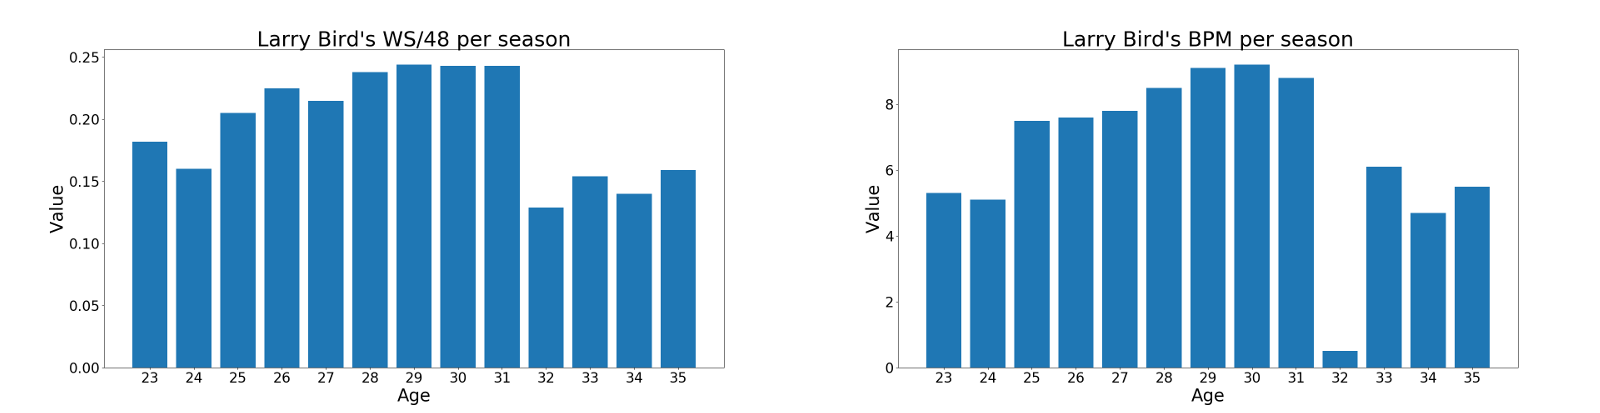
\includegraphics[scale=0.30]{bird.png}
\end{center}
\caption{Bird's WS/48 and BPM per season}
\label{plt:bird}
\end{figure}

\begin{figure}[h!]
\begin{center}
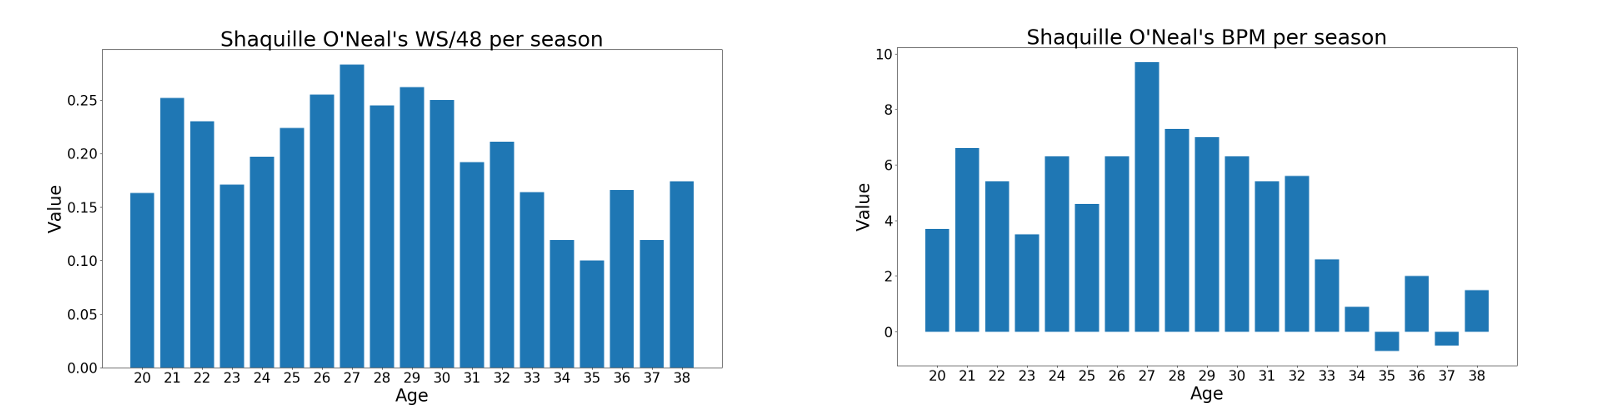
\includegraphics[scale=0.30]{shaq.png} % 2 x 800px and 413px
\end{center}
\caption{Shaq's WS/48 and BPM per season}
\label{plt:shaq}
\end{figure}

\begin{figure}[h!]
\begin{center}
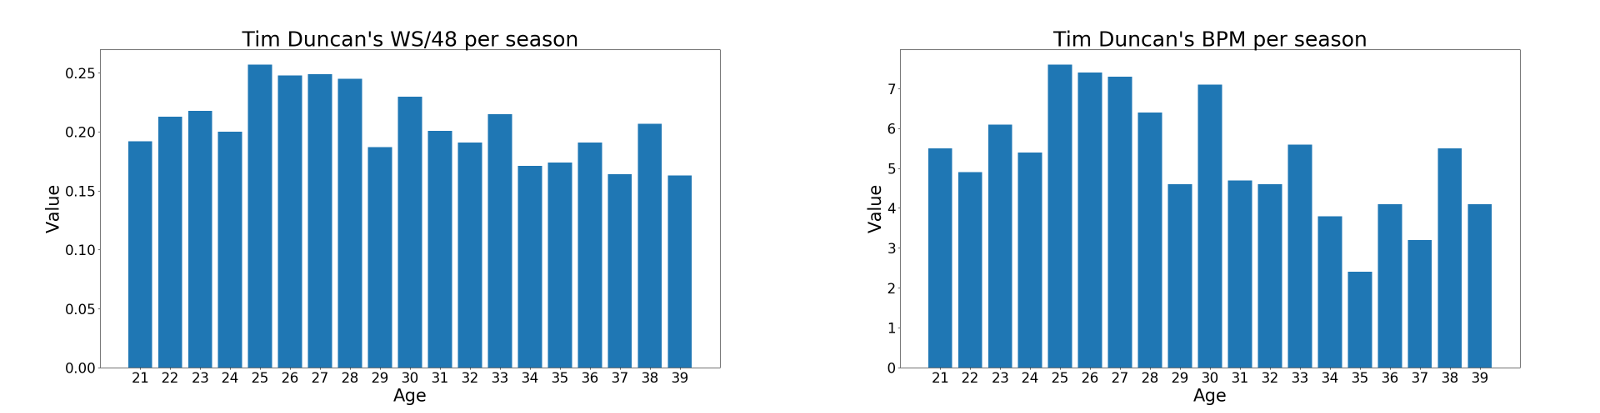
\includegraphics[scale=0.30]{duncan.png}
\end{center}
\caption{Duncan's WS/48 and BPM per season}
\label{plt:duncan}
\end{figure}

In the next step of determining prime of players, I checked at what age do players win awards, such as \textit{Regular season MVP}, \textit{Finals MVP}, \textit{DPOY} and \textit{Sixth man of the year} (\textit{SMOY}). Plots are shown in figure \ref{plt:awards}. Every plot but the plot for Defensive player of the year is somewhat similar. In those plots the number of awards players won while in their late twenties and early thirties is greater than number of awards in other years. Defensive player of the year award plot is different, where players aged from 23 to 31 won with roughly the same frequency, with an exception of players who were 28 (highest value) and 27 years old when they won. After that, there is a significant drop. These plots are showing us that the best players in the season are usually ones between 26 and 31 years old. But those players are stars and superstars. What about an average player?

\begin{figure}[h!]
\begin{center}
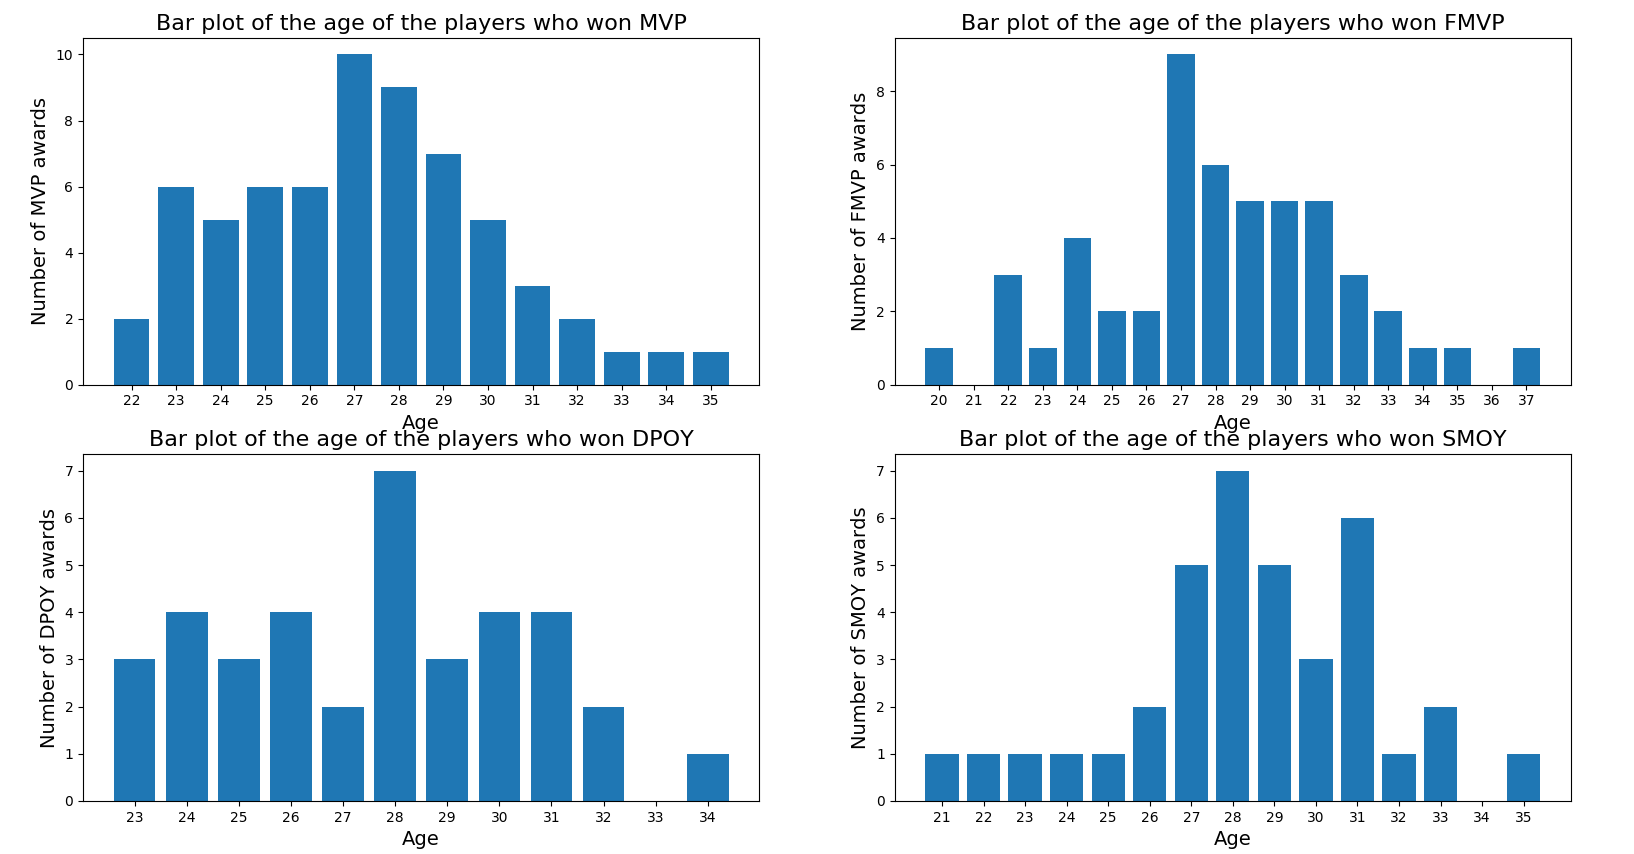
\includegraphics[scale=0.3]{awards_plots.png}
\end{center}
\caption{Age of award winners}
\label{plt:awards}
\end{figure}

After that, I checked age of players who played in the NBA. Results can be seen in figure \ref{plt:age_hist}. Note that there are two histograms. One represents every player who played in the NBA. The other is filtering out every player that has played in less than 35 games and less then 15 minutes per game. Those players are filtered out because I don't consider them regular contributors for the team they are playing for. The reason behind that is that they are probably not skilled enough, and possibly not in their prime, so they might not be important. Also, I just wanted to check on their histogram as well. Data used only takes into account players in the so-called \textit{Three-point era}. which began in 1979/80 season, the first season with 3-point line, and last till this day.

\begin{figure}[h!]
\begin{center}
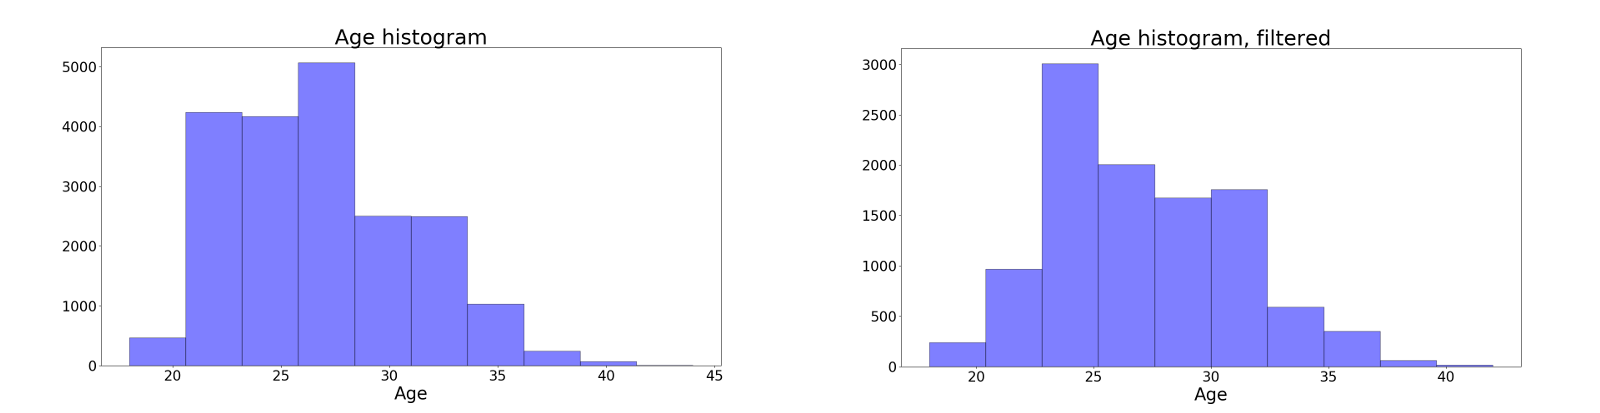
\includegraphics[scale=0.3]{age_histograms.png}
\end{center}
\caption{Age histograms}
\label{plt:age_hist}
\end{figure}


In the left histogram, unfiltered one, most of the players are in between 21 and 28 years old. That makes sense because players are usually drafted when they are younger than 25, and after rookie contracts expire and they are not good enough, they are out of the league. Histogram on the right has way lower number of players youger than around 23 years old. The reason behind that is that rookies aren't usually contributors right away because they need some time to develop.   The difference in number of players that are above 28 years old in unfiltered and filtered data is not that large. That is the case because players above that age are usually good players and they might be good because they are in their prime. That trend continues on both histograms until the significant drop somewhere after players reach 32 or 33. That might happen because they are simply not serviceable anymore and because of that cannot find teams to sign with. To conclude this paragraph, number of players is rising ar first, until the age of 28 (or 25 for filtered players). After that, there are two significant drops.

Now, I can try to estimate prime of an average player with statistics. First, I checked traditional stats. Bar plots for four stats are shown, PTS, FG, FGA and FT. Simply, it is expected from a player in his prime to shoot and score more than in his non-prime seasons. Note that values represented on a y-axis are averages per season, not per game! In figure \ref{plt:totals_age} every player from the three-point era is taken into account while players represented in the figure \ref{plt:totals_age_filtered} are the ones I consider contributors (minutes per game $>$ 15 and games played $>$ 35).

\begin{figure}[h!]
\begin{center}
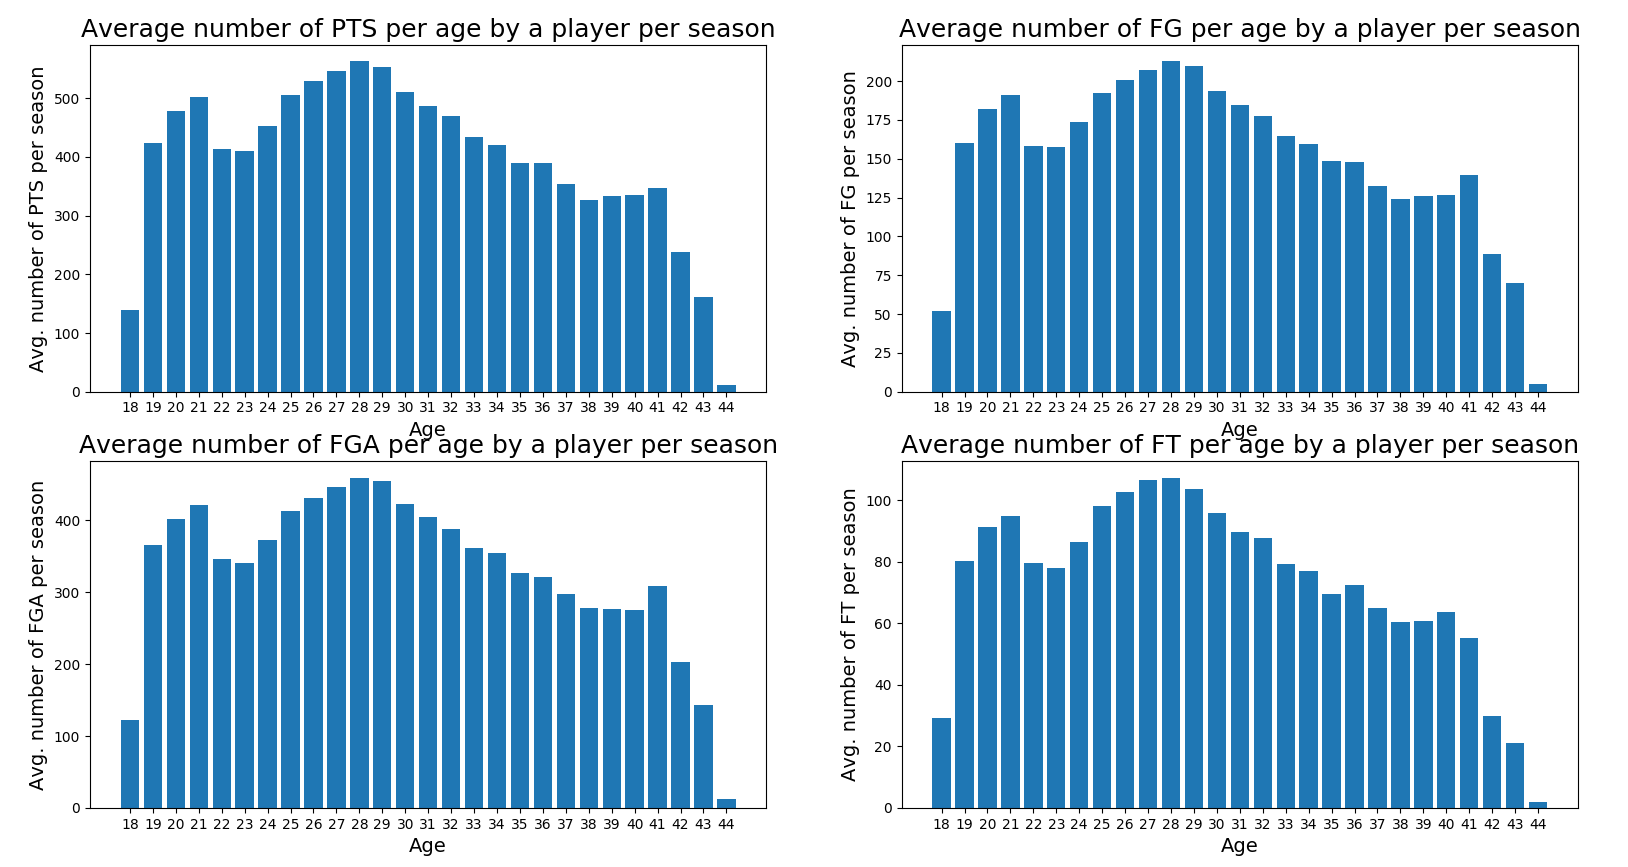
\includegraphics[scale=0.3]{traditional_stats_per_age.png}
\end{center}
\caption{Season totals averages per age unfiltered}
\label{plt:totals_age}
\end{figure}

\begin{figure}[h!]
\begin{center}
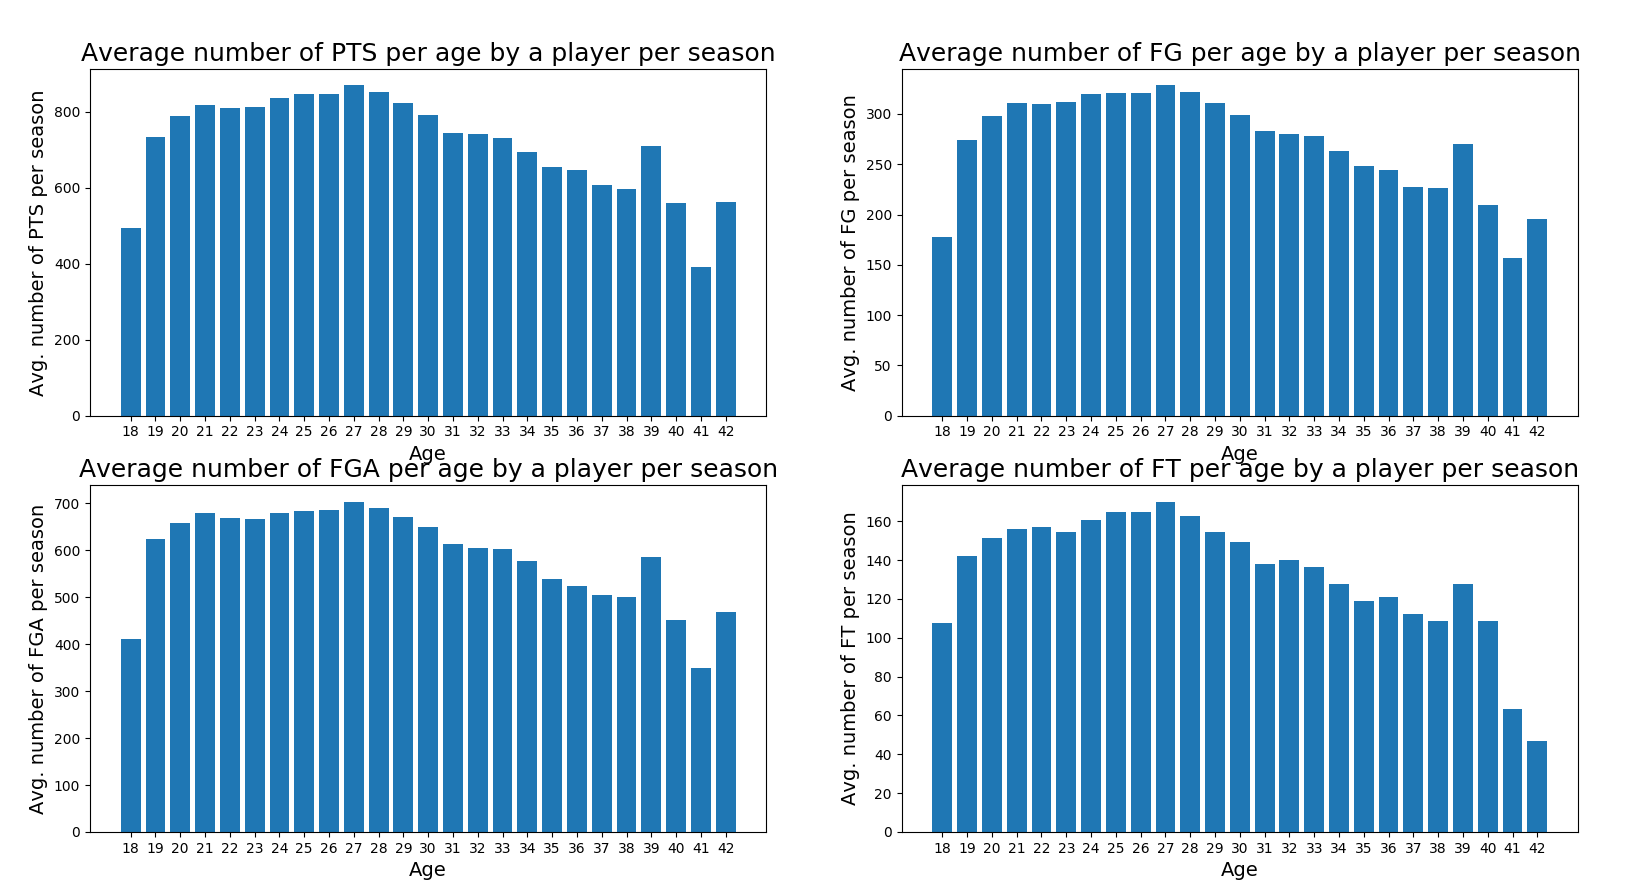
\includegraphics[scale=0.3]{traditional_stats_per_age_filtered.png}
\end{center}
\caption{Season totals averages per age filtered}
\label{plt:totals_age_filtered}
\end{figure}

Both figures are somewhat similar. Values for players aged from 26 to 30 or maybe 31 are higher than for any other age, with a significant drop after that. Both figures show peaks at a similar age, 28 for unfiltered data and 27 for filtered. So it's good thing to consider that prime of an average player is actually in late twenties/early thirties. The main difference can be seen in values for players that are younger than 25. Unfiltered data has easily noticeable difference between values for players that are 21 and 22 years old. Reason behind that is probably draft. Promising players are drafted earlier, often before they are 20, while a lot of players with lower upside decide to devlop in college and try to enter the league later. Those players are the reason why the values are lower for certain age. From plots with filtered data we can observe that those players are not contributing right away, so lower values are, while still there, not so emphasized.

Advanced stats are better than traditional and hold more information about how good a certain player is. So, I did similar thing as in the paragraphs before, but now with the advanced stats. Stats chosen are PER, WS, BPM and VORP. Bar plots for unfiltered players are shown in figure \ref{plt:advanced_age}, while bar plots after filtering are in figure \ref{plt:advanced_age_filtered}.


\begin{figure}[h!]
\begin{center}
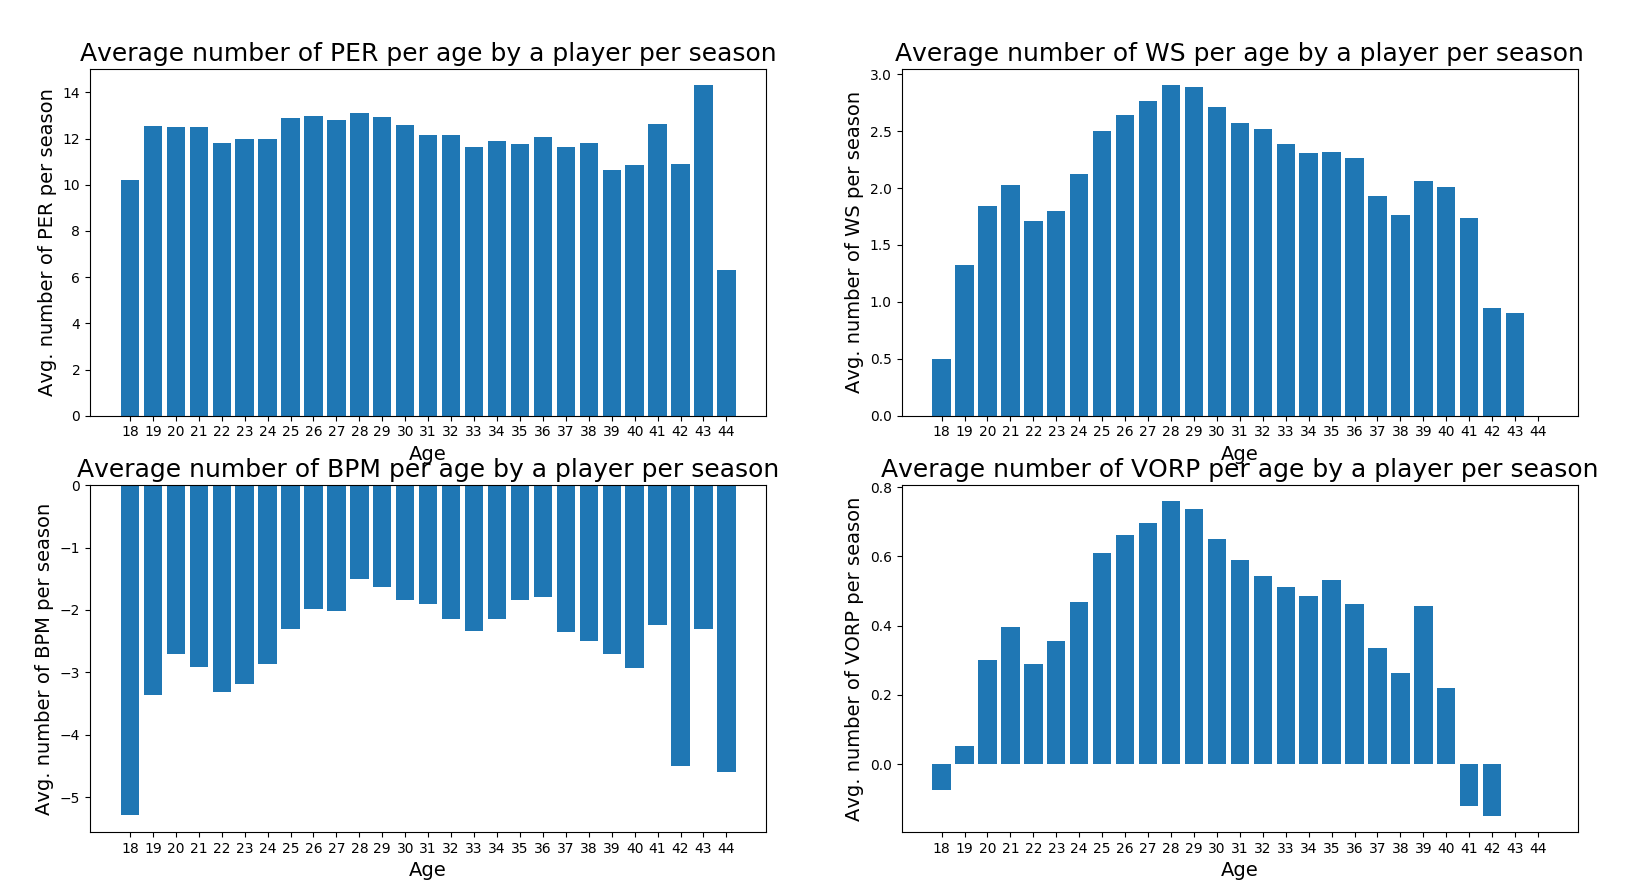
\includegraphics[scale=0.3]{advanced_stats_per_age.png}
\end{center}
\caption{Advanced stats averages per age unfiltered}
\label{plt:advanced_age}
\end{figure}

\begin{figure}[h!]
\begin{center}
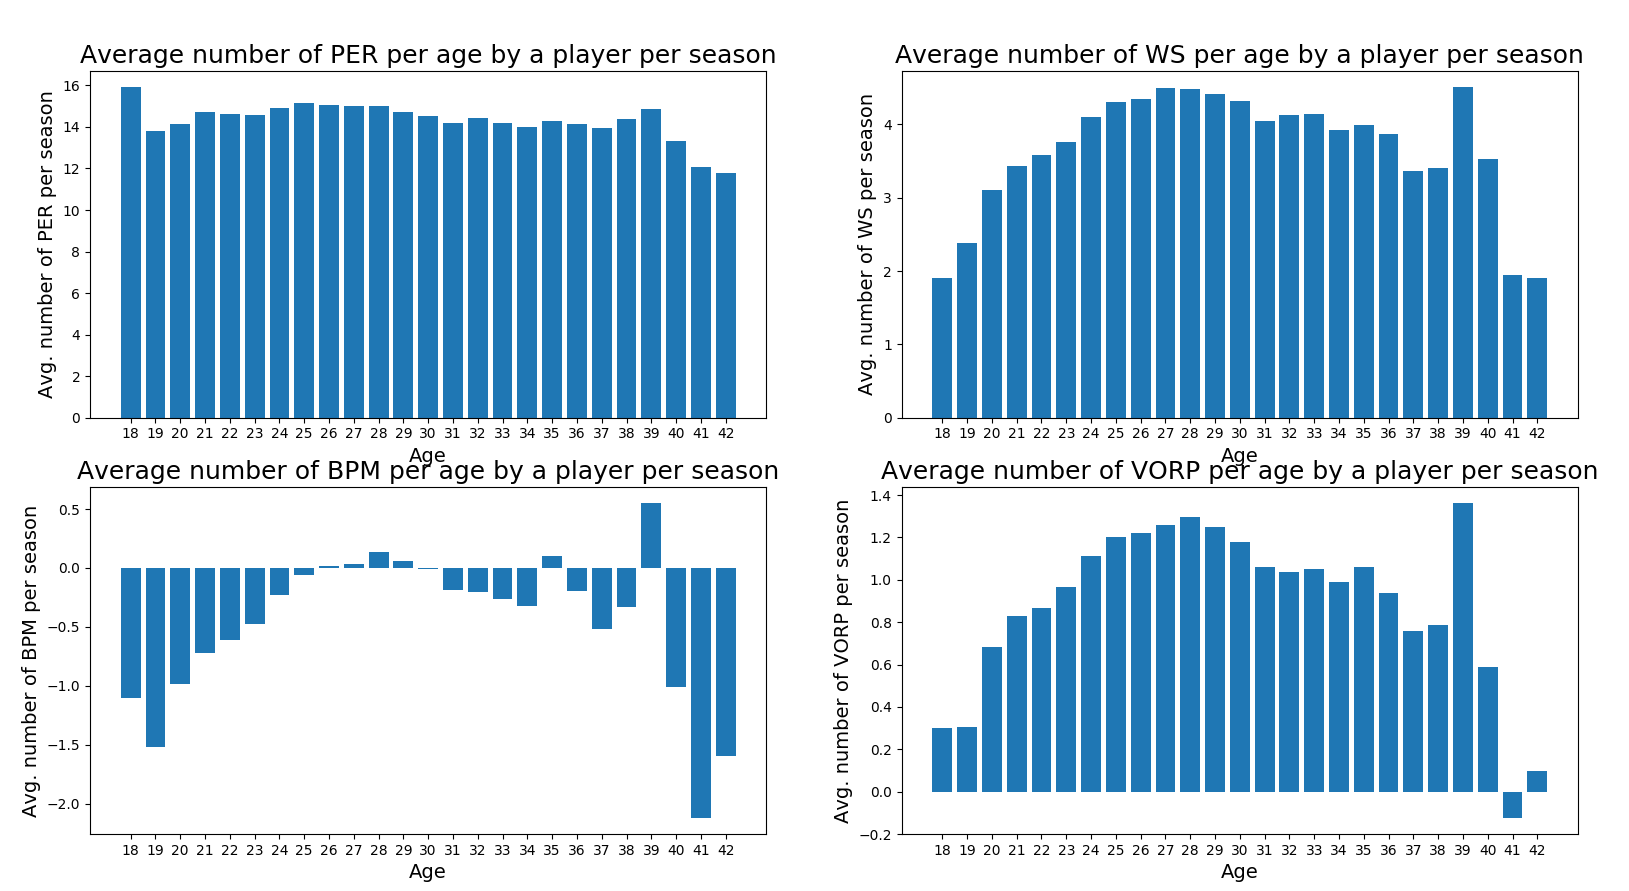
\includegraphics[scale=0.3]{advanced_stats_per_age_filtered.png}
\end{center}
\caption{Advanced stats averages per age filtered}
\label{plt:advanced_age_filtered}
\end{figure}

These plots are way more interesting. First, PER bar plot, for both filtered and unfiltered data, is somewhat similar to the ones with traditional stats, with the same results. Plots for WS and VORP are having spike in values from 26 to 31 on y-axis and lower values from the sides. That radius with higher values contains prime years of an average player. Plot for BPM is, interestingly, negative for unfiltered data, and with some positive values for filtered data. Highest values for BPM are from players from 25 to 36 years old. Some of the plots that are showing advanced data have high value for players 39 years old, which is interesting. Those players were usually very good in their prime, and because of that they were usually good when they were older, just not that good anymore, and in usually lower minutes per game. Also, not many players play by that age, so the average might be high because there is a small number of players, none of which are bad.

Taking all mentioned things into a consideration, age when players are usually winning awards and age when the players are statistically better than in any other age, conclusion is that an average player enters into prime at around his \textbf{25th} year, and exits when he is around \textbf{31}, with kinda significant drop after that. Peak season happens when player is from \textbf{27 to 29} years of age, somewhere in the middle of their prime.

\section{Nikola Joki\' c analysis}
\label{jokic}

Nikola Jokić was drafted by the Denver Nuggets as a 41st overall pick in the 2014 NBA draft. One year later, he signed with the team, and soon became the starting center, and the team's best player. Let's see some of his stats per season through his career. Traditional stats are shown in the figure \ref{plt:trad_jokic} while advanced stats are shown in figure \ref{plt:adv_jokic}.

\begin{figure}[h!]
\begin{center}
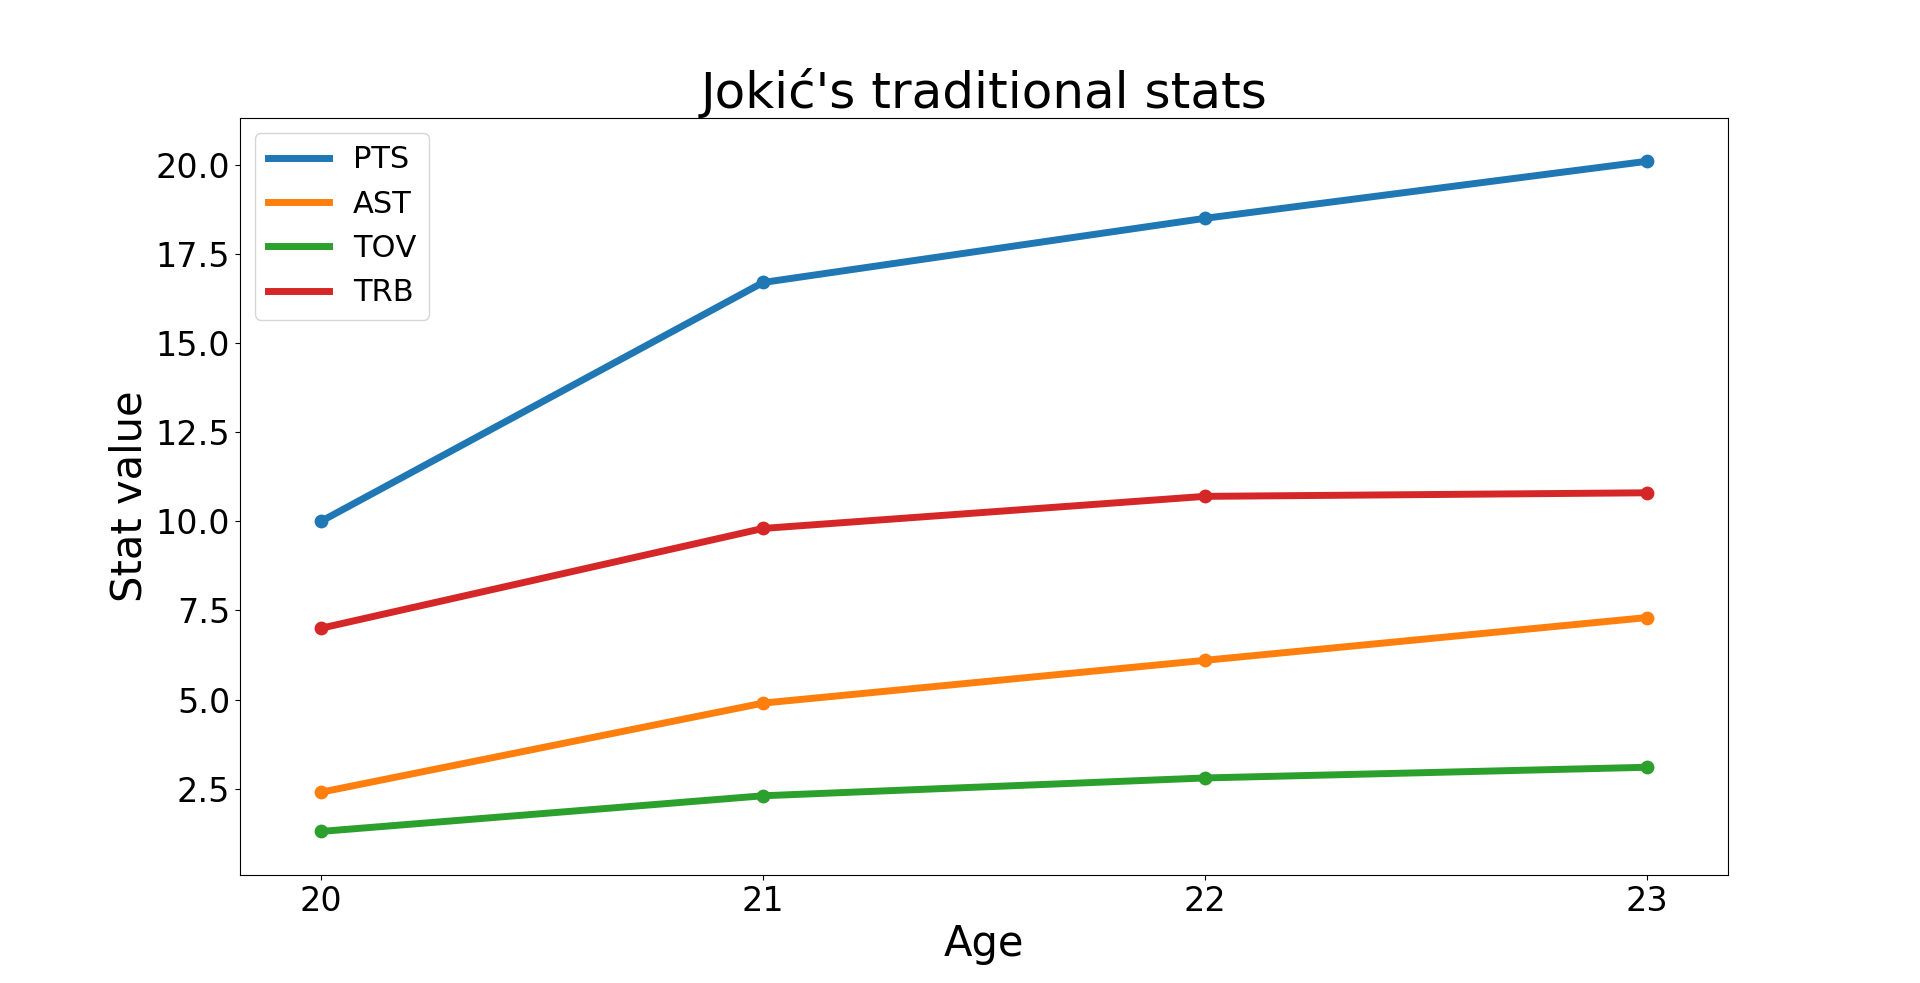
\includegraphics[scale=0.25]{jokic_plot_traditional.png}
\end{center}
\caption{Traditional stats by Joki\' c per season}
\label{plt:trad_jokic}
\end{figure}

\begin{figure}[h!]
\begin{center}
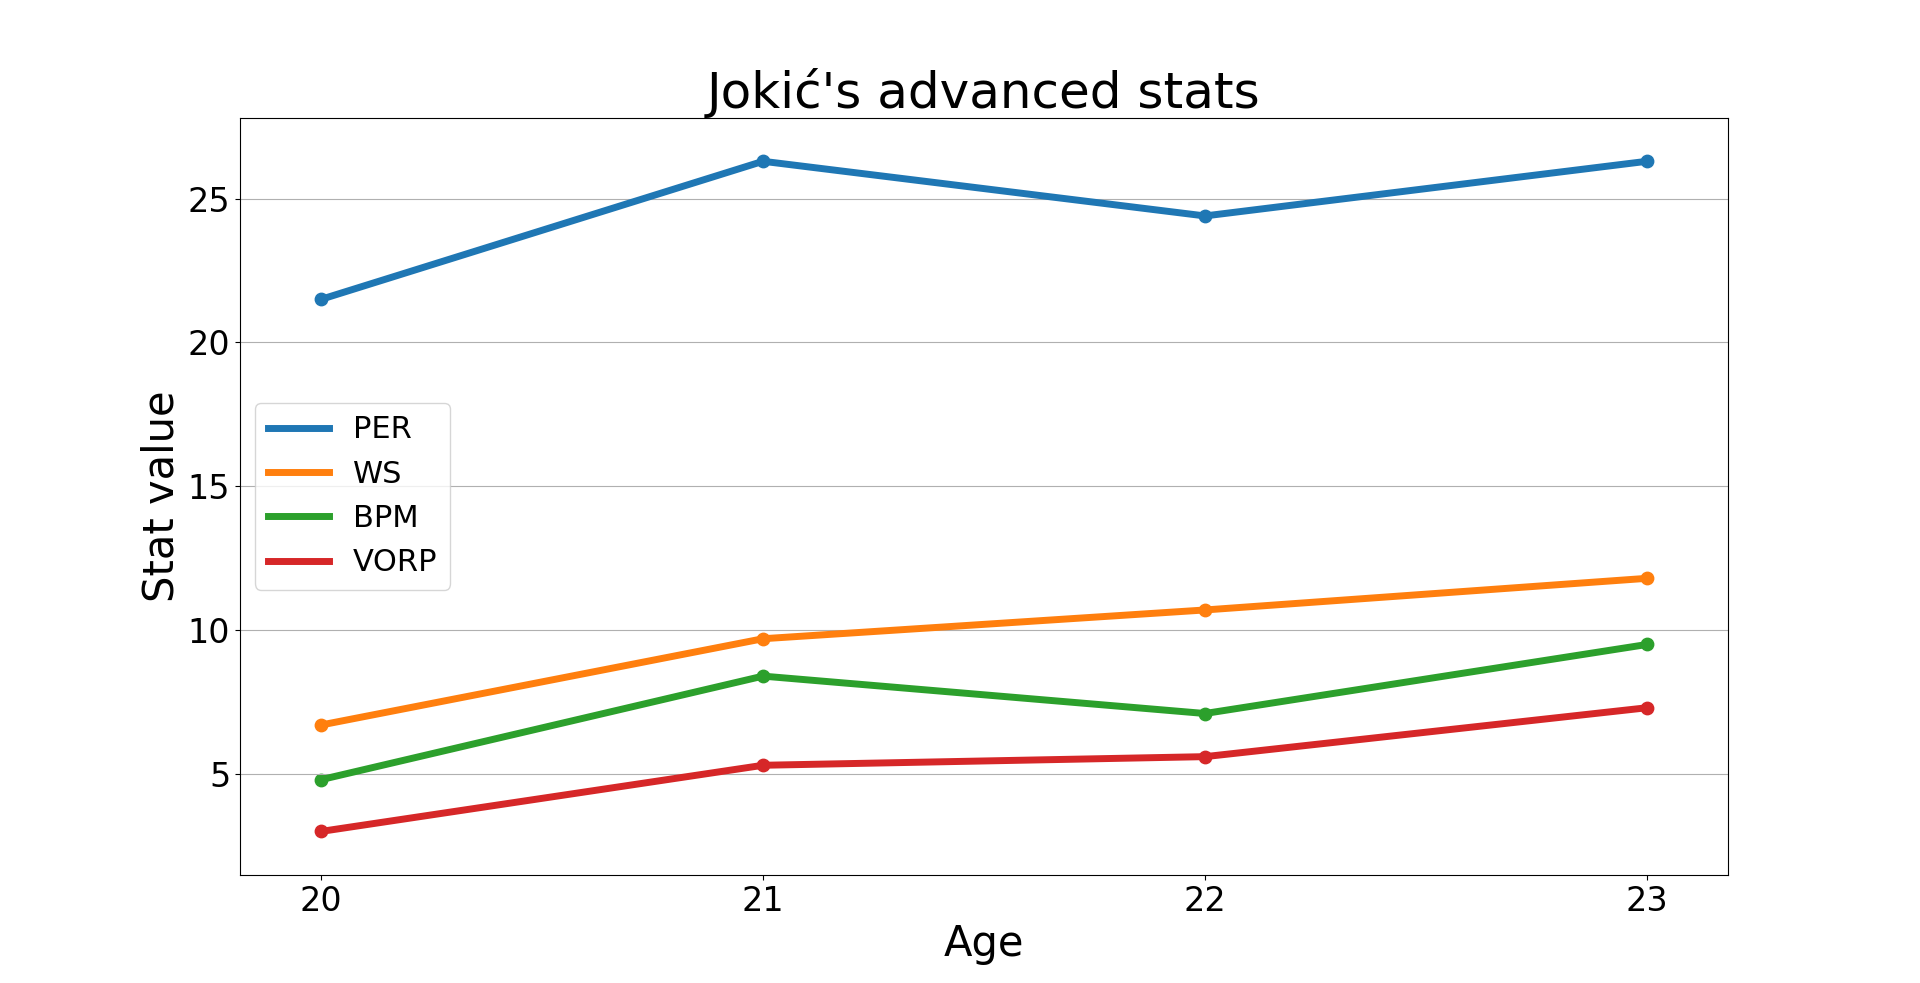
\includegraphics[scale=0.25]{jokic_plot_advanced.png}
\end{center}
\caption{Advanced stats by Joki\' c per season}
\label{plt:adv_jokic}
\end{figure}

As we can see, the stats are getting better as he age, and are very good in his forth season (2018-19) where he earned spot on the \textbf{1st All-NBA} team and the \textbf{All-star} selection.

\subsection{Did he deserve 1st team All-NBA in the 18-19 season?}
\label{subsec:jokic_all_nba}

Let's start this subsection with a note that All-NBA teams are \textit{selected by voters}, and \textbf{not} purely by stats. That means that the players who are statistically very good might not get All-NBA team selection, if, for example, a team they play for isn't successful, although that's unlikely. Also, player doesn't have to be one of the five best players in the league to end up on the 1st All-NBA team, he just have to be the best, according to a voter, at his position. The All-NBA team consists of two guards, two wings and one center. In the 2018-19 season, Nikola Joki\' c was on the 1st All-NBA team. Did he \textit{statistically} deserve it?

Joki\' c is a \textit{center}, and there is only one center on the 1st All-NBA team, so I just have to compare his stats with the stats of the other centers. In the 2018-19 season, Joki\' c played in 80 games, averaging 31.3 MPG, 20.1 PPG, 10.8 RPG and 7.3 APG on 0.51 FG\%, 0.31 3P\%, 0.82 FT\% shooting splits. Here is how it compared to other \textbf{centers} in the same season. Plot chosen to represent this data is Box plot \cite{boxplots}, because we want to see whether Joki\' c is, and how much, better than other centers.


\begin{figure}[h!]
\begin{center}
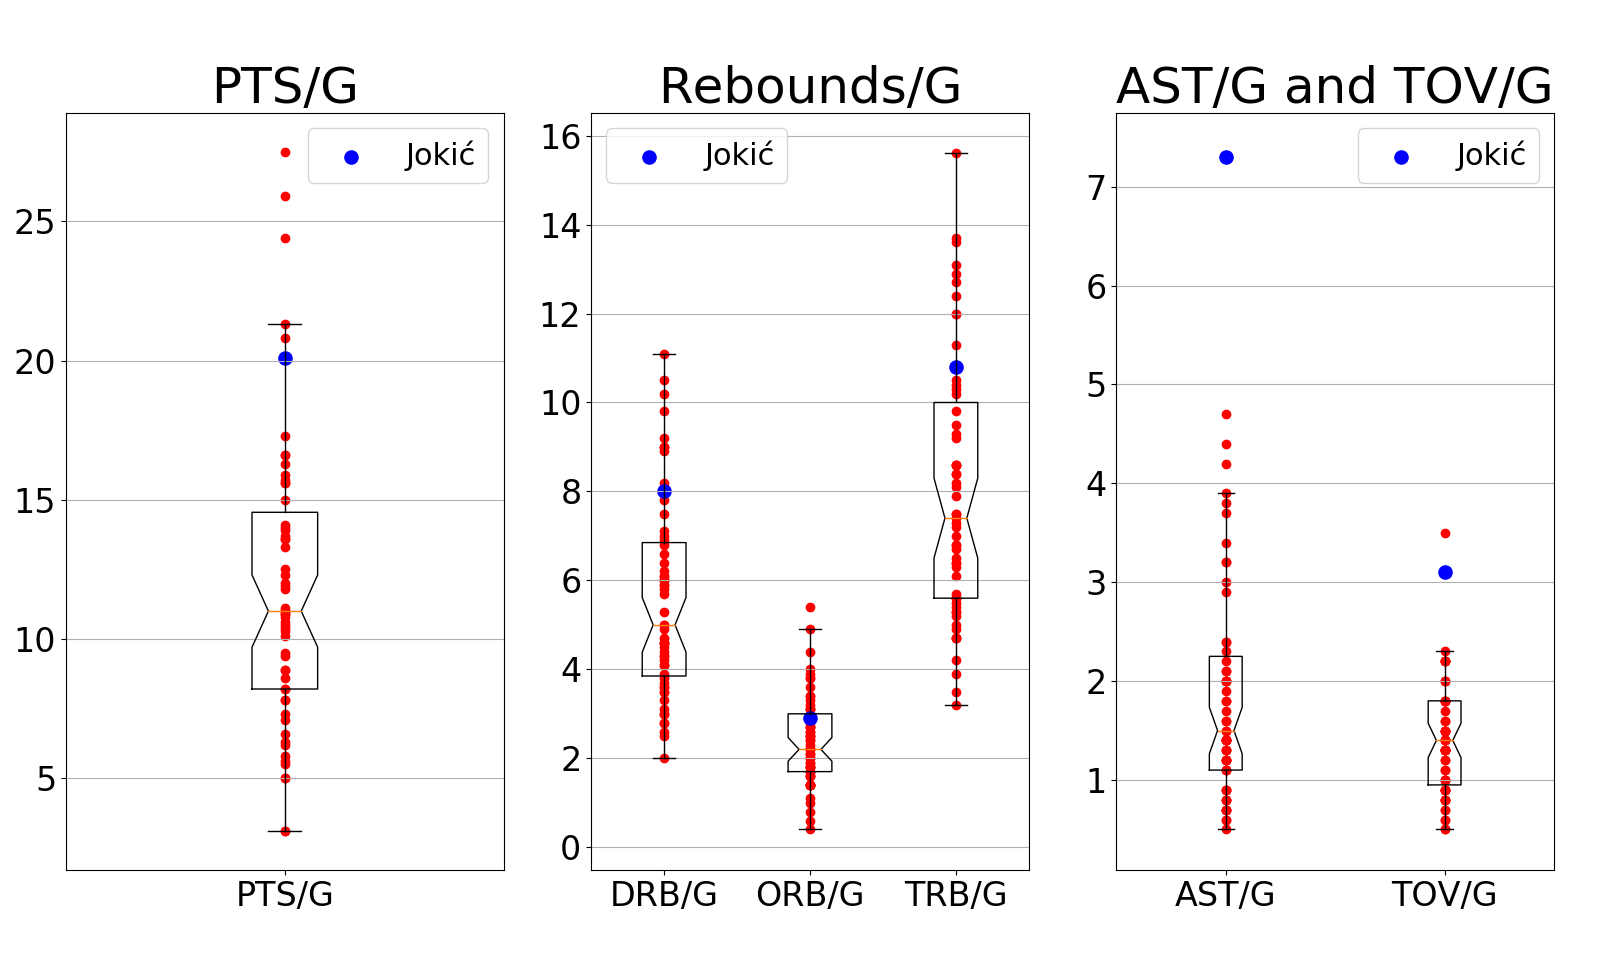
\includegraphics[scale=0.30]{centers_traditional.png}
\end{center}
\caption{Box plots of the traditional stats by centers in 2018-19 season}
\label{plt:centers_trad}
\end{figure}

These stats are showing that Joki\' c really was one of the best centers in the league. Although not the best scorer or rebounder (but still very good), he had by far the most assists, almost three more than the second placed Marc Gasol, which is probably the reason why he had the 2nd most turnovers. As we have seen, traditional stats are almost always inferior to advanced when evaluating how good a certain player is. That is why the next step is to check out Joki\' c's, (figures \ref{plt:centers_adv} and \ref{plt:centers_bpm}) and compare it with others.

\begin{figure}[h!]
\begin{center}
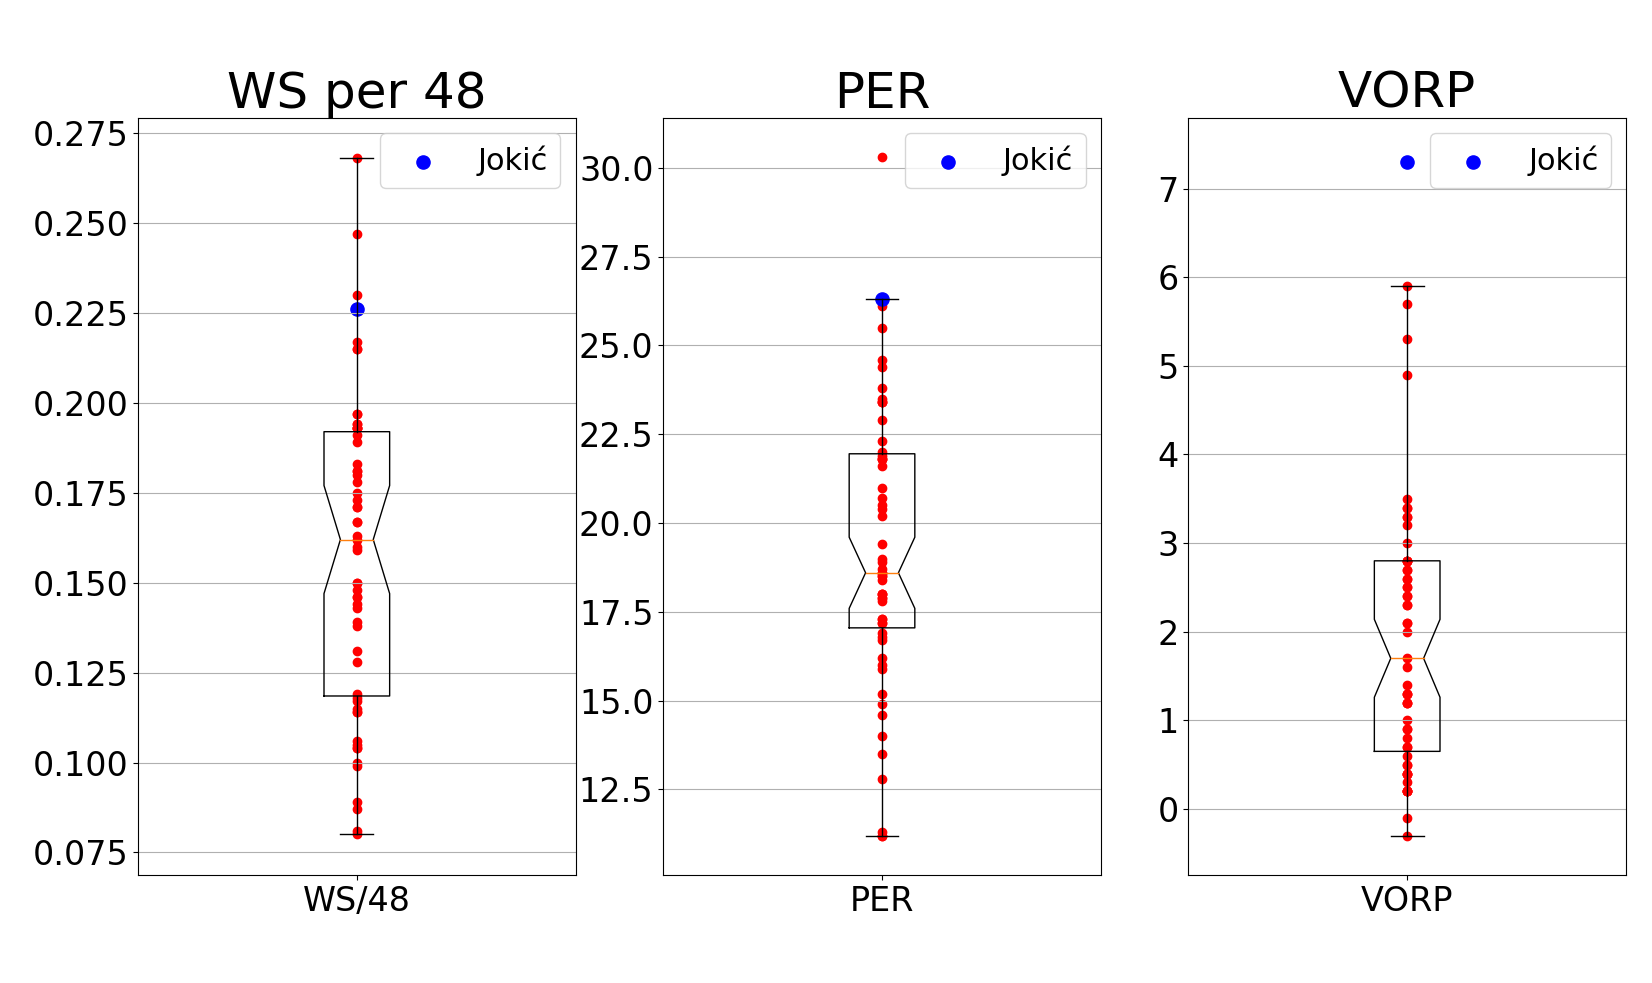
\includegraphics[scale=0.30]{centers_advanced.png}
\end{center}
\caption{Box plots of the advanced stats by centers in 2018-19 season}
\label{plt:centers_adv}
\end{figure}

\begin{figure}[h!]
\begin{center}
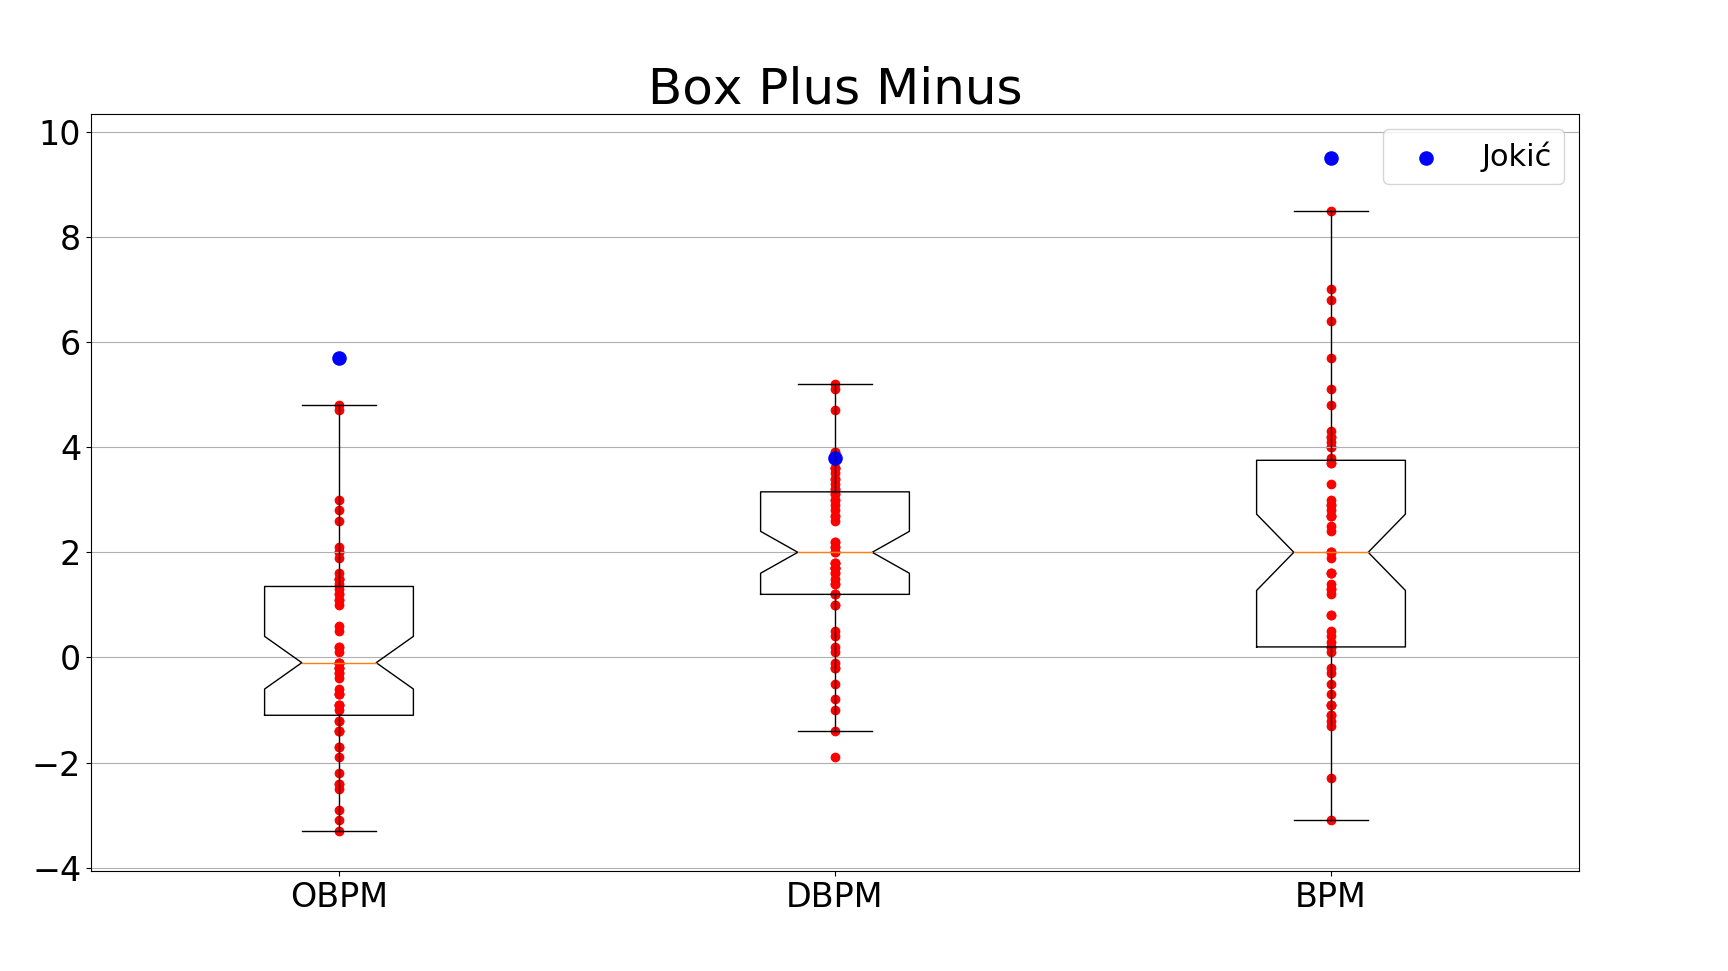
\includegraphics[scale=0.30]{centers_bpm.png}
\end{center}
\caption{Box plots of the Box Plus Minus stats by centers in 2018-19 season}
\label{plt:centers_bpm}
\end{figure}

Among centers, he was ranked high on WS/48 (4th), PER (2nd) and DBPM (5th) and is \textbf{first} in VORP (3rd in the league), OBPM (7th in the league) and BPM (3rd in the league). He dominated advanced statistics, not only when compared to the other players at his position, but also when compared to the best players in the NBA in that season. From this, it is not hard to determine that Nikola Joki\' c statistically deserved to be on the All-NBA 1st team! Of course, that does not mean that other centers weren't, but it means that voters had good reasoning behind their decision. The thing that certainly helped was that Denver Nuggets, led by him as the best player, were 2nd seeded team in the Western conference.

\subsection{Passing}
\label{subsec:jokic_passing}

The thing Joki\' c is most known for is definitely his passing ability, the thing that the average center isn't usually that good in. In this section I will take a look at his passing statistics, and compare it to other players (not just centers) from the NBA history. But first, let's see how his passing compares to the other centers. As we have seen in the previous section, his AST/G number (7.3) was by far the best in the league at his position. How many centers in the history averaged something similar? Table \ref{tab:centers_ast_g} contains every season where a center averaged more than six AST per game.

\begin{table}[h!]
\begin{center}
\begin{tabular}{|c|c|c|c|c|} \hline
\textbf{Player} & \textbf{Age} & \textbf{Season} & \textbf{Minutes per game} & \textbf{Assists per game} \\ \hline
Wilt Chamberlain & 31 & 1967-68 & 46.8 & 8.6 \\ \hline
Wilt Chamberlain & 30 & 1866-67 & 45.5 & 7.8\\ \hline
Nikola Jokić & 23 & 2018-19 & 31.3 & 7.3 \\ \hline
Nikola Jokić & 22 & 2017-18 & 32.6 & 6.1 \\ \hline
\end{tabular}
\caption{Centers with more than six assists per game in a season}
\label{tab:centers_ast_g}
\end{center}
\end{table}

Yes, only two centers in the \textbf{history} of the NBA menaged to average more than six assists per game in a season. Number of seasons with decreased AST/G in a season by a center, \textbf{five}, is 21, by only 13 players. Wilt Chamberlain appears on that expanded list four times, ranked 1st, 2nd, 15th, 20th, while number of Nikola Joki\' c's such seasons remains the same, two, with 3nd and 4th spots. Note that Joki\' c's third highest AST/G is 4.9, so he misses new list by a tiny margin.

The best way to compare players would be per possession stats, but those stats were measured from 1973-74 season, some seasons after Wilt set his personal record in AST/G. Instead of that we can only compare per minute production (table \ref{tab:jokic_wilt_per_36}). In this category, Joki\' c is better than Chamberlain, with the significant difference. Note that there are 5 centers (9 seasons in total), that played more than 15 MPG and 35 G in a season and menaged to average more than six AST per 36, with Joki\' c being the first on that list, and only one with more than seven AST per 36. He is also 4th and 7th, while Chamberlain takes 5th and 8th spots.

\begin{table}[h!]
\begin{center}
\begin{tabular}{|c|c|c|c|c|} \hline
\textbf{Player} & \textbf{Age} & \textbf{Season} & \textbf{Minutes per game} & \textbf{Assists per 36} \\ \hline
Nikola Jokić & 23 & 2018-19 & 31.3 & 8.3 \\ \hline
Nikola Jokić & 22 & 2017-18 & 32.6 & 6.7 \\ \hline
Wilt Chamberlain & 31 & 1967-68 & 46.8 & 6.6 \\ \hline
Wilt Chamberlain & 30 & 1866-67 & 45.5 & 6.2 \\ \hline
\end{tabular}
\caption{Joki\' c's and Chamberlain's AST per 36 minutes}
\label{tab:jokic_wilt_per_36}
\end{center}
\end{table} 

Not only Joki\' c has hight AST per 36 minutes number, he is also at the top for AST per 100 possessions stat. In fact, out of top five AST per 100 seasons by a center (table \ref{tab:centers_ast_per100_top5}), Joki\' c has three! He is ranked 1st, 3rd and 5th. He is also the only center with more than 10 AST per 100, with 11.4, a significant diference to a second-placed Vlade Divac. Note that Joki\' c's rookie season, although not elite, still cracks top 100, at 90th spot.

\begin{table}[h!]
\begin{center}
\begin{tabular}{|c|c|c|c|c|} \hline
\textbf{Player} & \textbf{Age} & \textbf{Season} & \textbf{Assists per 100} \\ \hline
Nikola Jokić & 23 & 2018-19 & 11.4 \\ \hline
Vlade Divac & 35 & 2003-04 & 9.6 \\ \hline
Nikola Jokić & 22 & 2017-18 & 9.3 \\ \hline
Sam Lacey & 31 & 1979-80 & 8.9 \\ \hline
Nikola Jokić & 21 & 2016-17 & 8.6 \\ \hline
\end{tabular}
\caption{Best 5 of AST per 100 possessions by a center}
\label{tab:centers_ast_per100_top5}
\end{center}
\end{table}

High number of assists might not mean much, if a player turnovers the ball often. When compared to the other centers in TOV per 100 possessions, Joki\' c worst season (2018-19), at 4.9 TOV per 100, is ranked 59th, and it is his only season in the worst 100. This proves that Joki\' c might be \textbf{the best passing big man ever}. But what about other positions?

First, I compared his stats from 2018-19 to the ones of the other players from the same season. Result can be seen in figure \ref{plt:ast_tov_g}. Bottom right corner is good, top left corner is bad. Not only he is among the best passers in the league, but he is mostly surrounded by point-guards.

\begin{figure}[h!]
\begin{center}
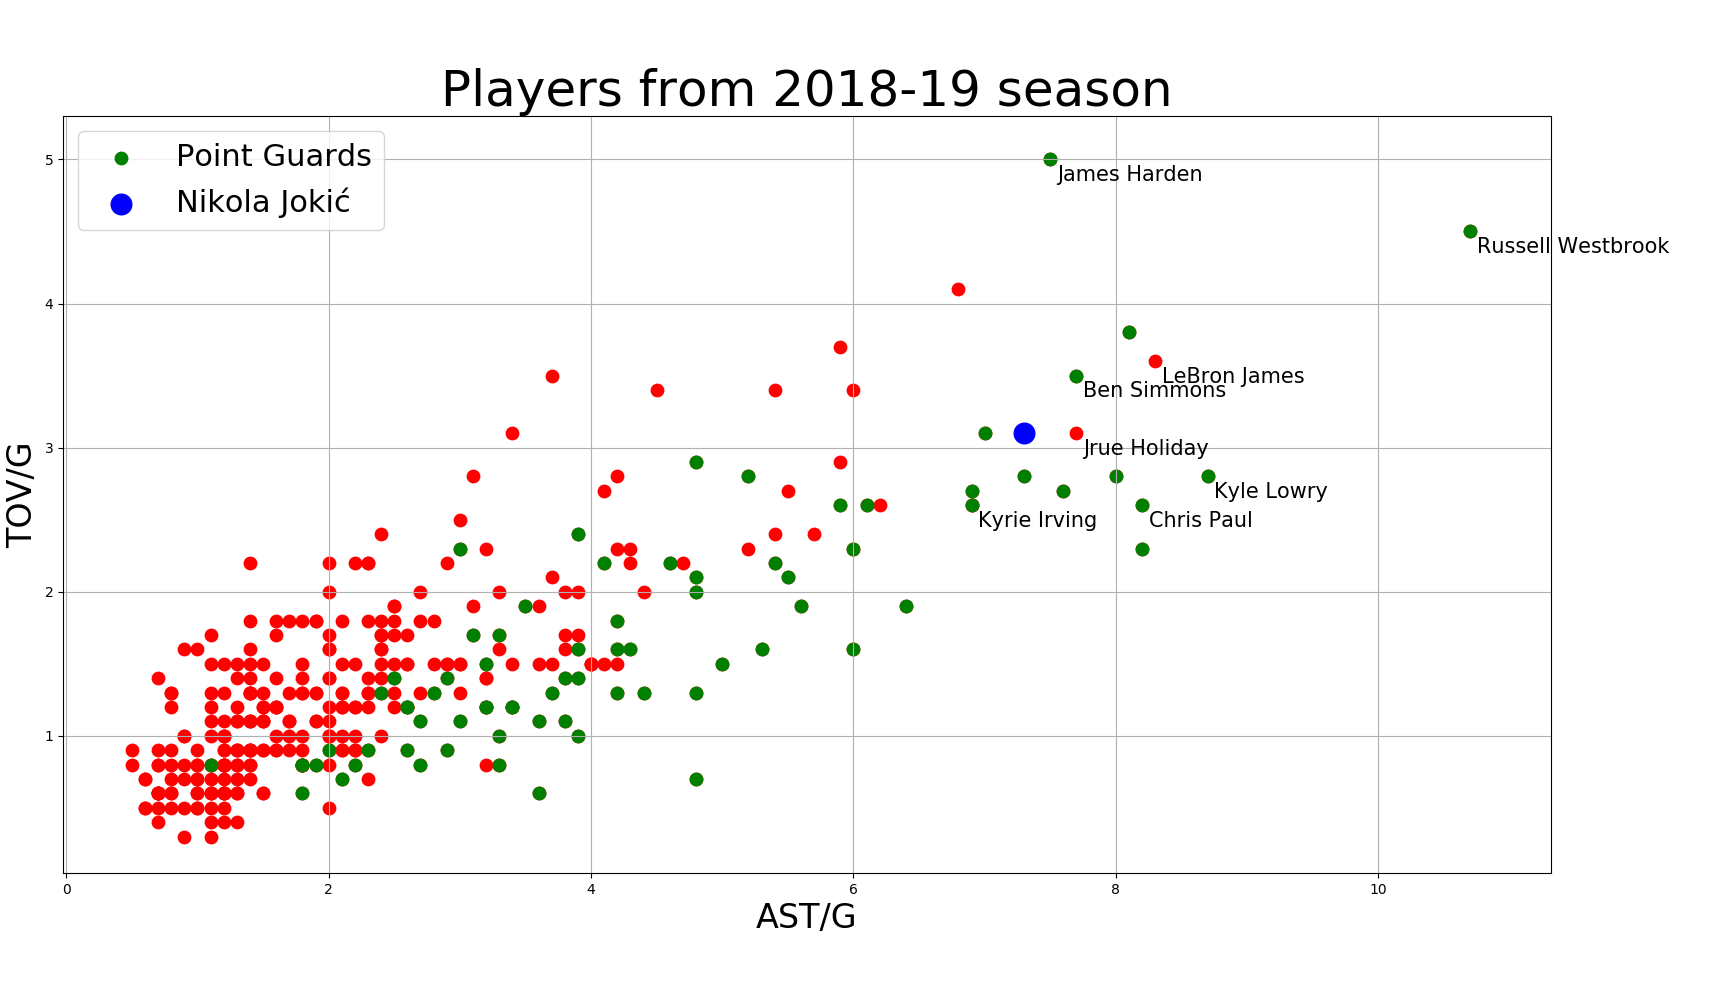
\includegraphics[scale=0.30]{ast_tov_g_2019.png}
\end{center}
\caption{AST/G to TOV/G for players from 2018-19 season (min 15 MP/G and 35 G)}
\label{plt:ast_tov_g}
\end{figure}

The figure \ref{plt:ast_tov_pct} is showing similar results, just this time, instead of AST and TOV per game, AST\% and TOV\% are used. Joki\' c had really good passing season, not just for a center, but overall!

\begin{figure}[h!]
\begin{center}
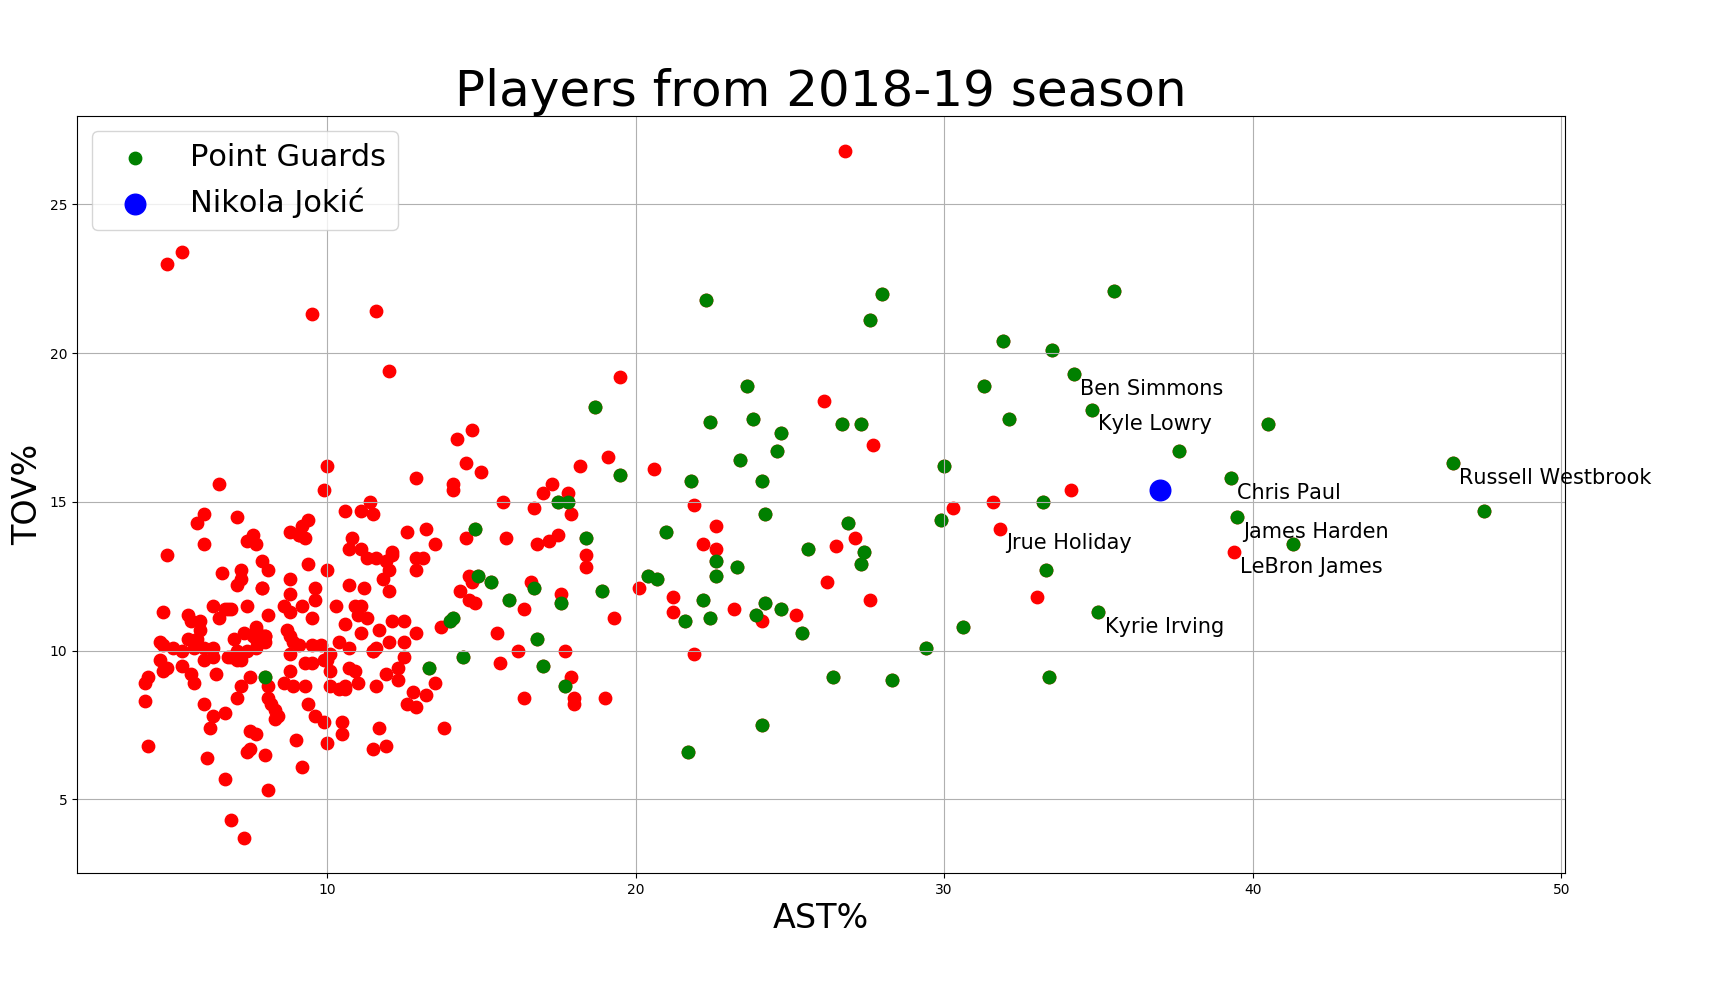
\includegraphics[scale=0.30]{ast_tov_pct_2019.png}
\end{center}
\caption{AST\% to TOV\% for players from 2018-19 season (min 15 MP/G and 35 G)}
\label{plt:ast_tov_pct}
\end{figure}

But what about NBA history? Let's take his best passing season and see how good it was compared to the every player from the 3-point era (figure \ref{plt:ast_tov_g_3p}). This is just the proof that his passing numbers are not center-like. His surroundings are made of non-centers exclusively. Plot is constructed in a way that it is good to be down and right, and bad to be up and left. Joki\' c is somewhere in the middle. That means that his numbers are not elite, but still solid.

\begin{figure}[h!]
\begin{center}
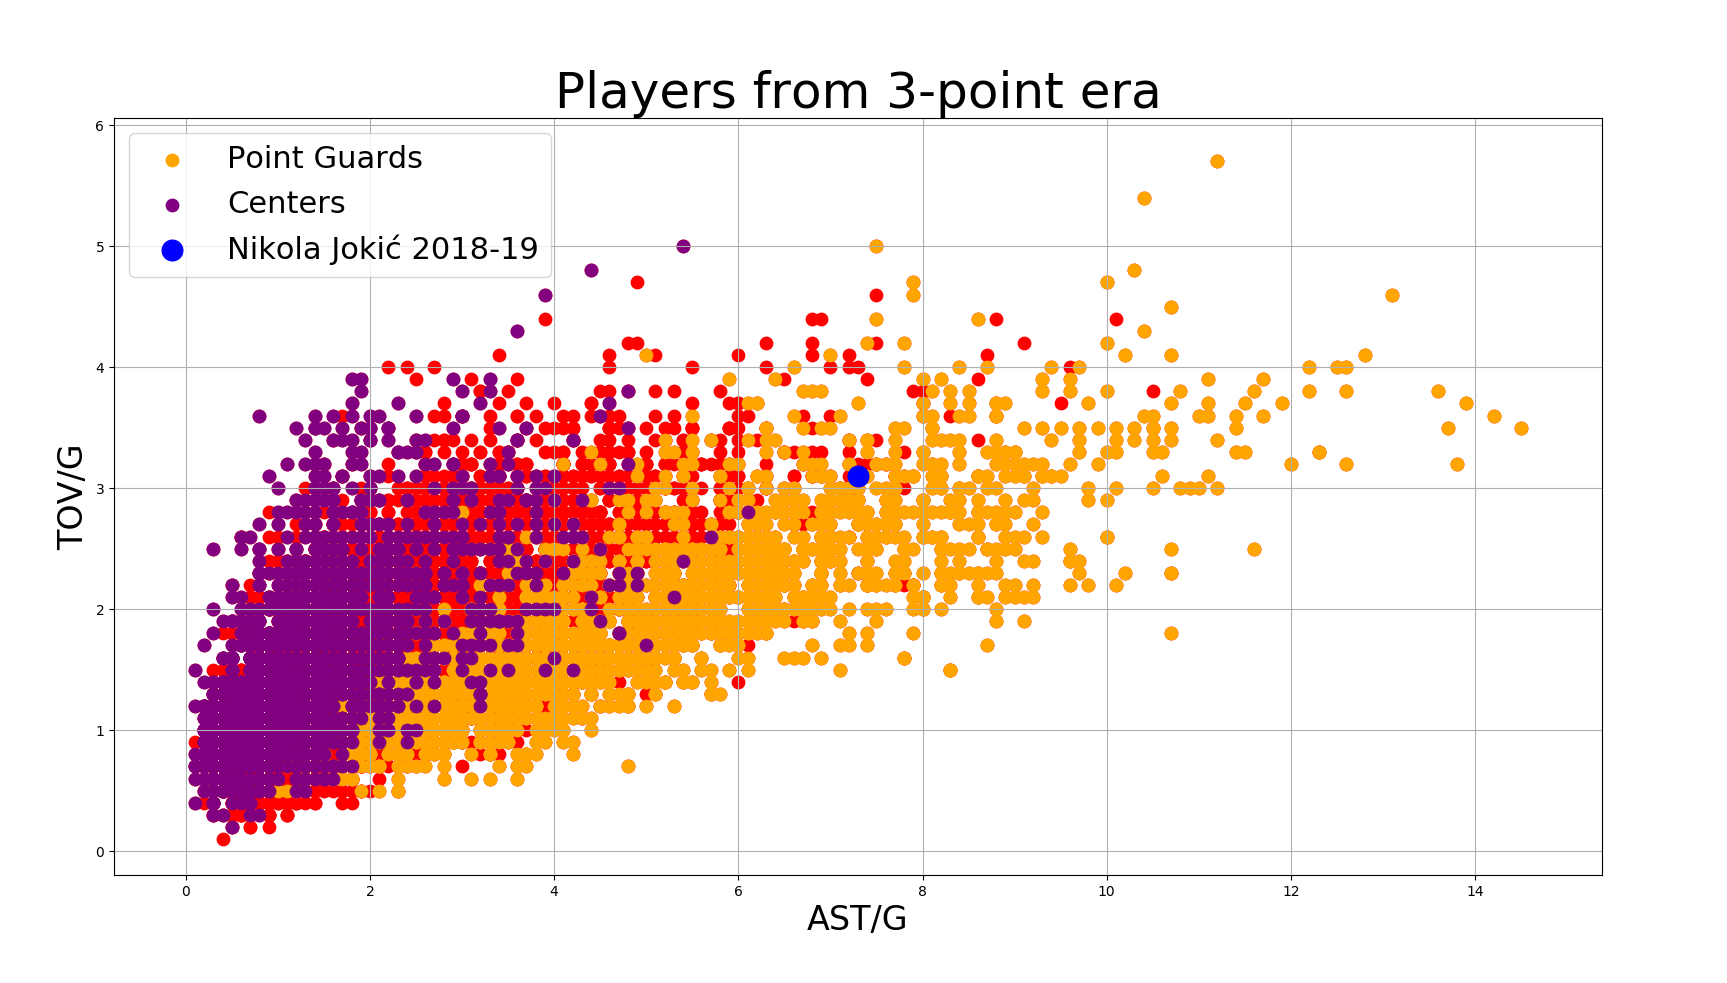
\includegraphics[scale=0.30]{ast_tov_g_3point_era.png}
\end{center}
\caption{AST\% to TOV\% for players from 3-point era (min 15 MP/G and 35 G)}
\label{plt:ast_tov_g_3p}
\end{figure}

On the second figure, that represents AST\% and TOV\% of the players from 3-point era, he moved down and right, which is good. Not only that, but it appears that there are fewer player between him and bottom-right corner than on the previous plot. That implies that his stats are a little bit better than what the per game numbers show.

\begin{figure}[h!]
\begin{center}
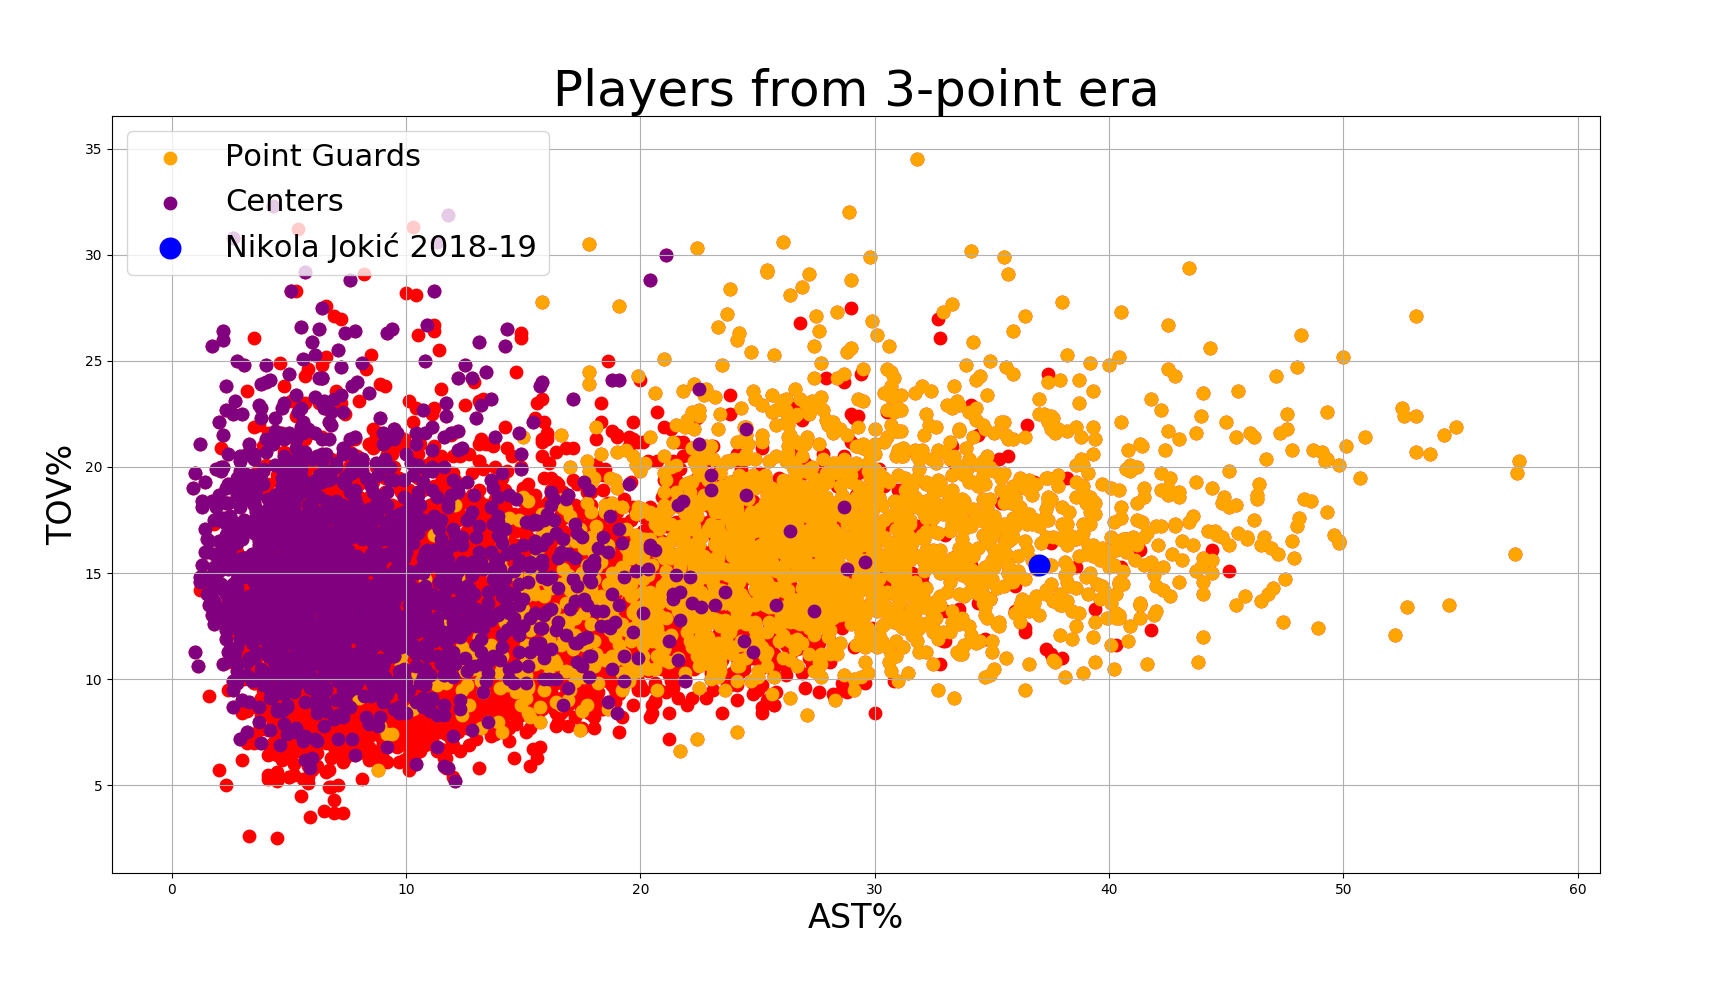
\includegraphics[scale=0.30]{ast_tov_pct_3point_era.png}
\end{center}
\caption{AST\% to TOV\% for players from 3-point era (min 15 MP/G and 35 G)}
\label{plt:ast_tov_pct_3p}
\end{figure}

To conclude this section, Nikola Joki\' c is absolutely best passing center ever. His passing numbers also look good when compared to the numbers of the elite passers, but are still inferior to them. Basically, he is passing like a starting caliber point guard.

In the end, let's say that AST and TOV aren't the only way to measure passing. Besides them, there are stats such as number of deflected passes, number of hockey assists and so on, all of which are helpful. Stats used in this section are very important for passing, but aren't prefect.

\pagebreak

\section{Moreyball}
\label{sec:moreyball}

Moreyball, named after Houston Rockets General manager Daryl Morey, is an offensive strategy in basketball that is based on taking just the most efficient shots, the shots that are worth the most points per possession. Those shots are 3-point shots, shots close to the basket and free throws. Let's see why those shots are more efficient than others.

Average Offensive rating in 2018-19 season in the NBA was 110.4. That means that an average offense scores 110.4 points per 100 possessions. In that same season, percentages of shots from the areas calculated by distance from the basket, according to the stats.nba.com, were:

\begin{itemize}
	\item Percentage of shots close to the basket (less than 8 ft.) is 0.579. That translates to 115.8 points per 100 possessions.
	\item Percentage of shots from 8 to 16 ft. is 0.412. That translates to 82.4 points per 100 possessions.
	\item Percentage of shots from 16 to 24 ft. is 0.401. That translates to 80.2 points per 100 possessions.
	\item Percentage of shots at the 3-point line (24+ ft.) is 0.357, with back court shots excluded. That translates to 107.1 points per 100 possessions.
	\item Percentage of \textbf{wide open} 3-point shots (where the nearest defender is at 6+ ft.) is 0.380. That translates to 114.0 points per 100 possessions.
	\item Percentage of a free throw shot is 0.776. That translates to 76.6 points per 100 possessions (one shot), 153.2 per 100 (two shots) or 229.8 per 100 (three shots).
\end{itemize}

From here, it is easy to conclude which shots produce more points per possession than the average. Those shots are either close to the basket, or three-pointers. Not only that, but the most efficient field goal a team can take is the one from less than 8 feet, because those shots are hard to miss. Also, two free throws per possession are extremely efficient. Notice how staggering difference is between average 3-point shot and three free throws, the obvious reason why fouling someone on three-point shot is extremely bad.

Because of that, most teams nowadays are trying to implement Moreyball. If we compare shot charts by teams from 2018-19 season, and shot chart from the same team just 6 years prior (2012-13 season), we will see noticeable difference (figure \ref{plt:shotcharts}). Teams used to shoot more mid-range shots.

\begin{figure}[h!]
\begin{center}
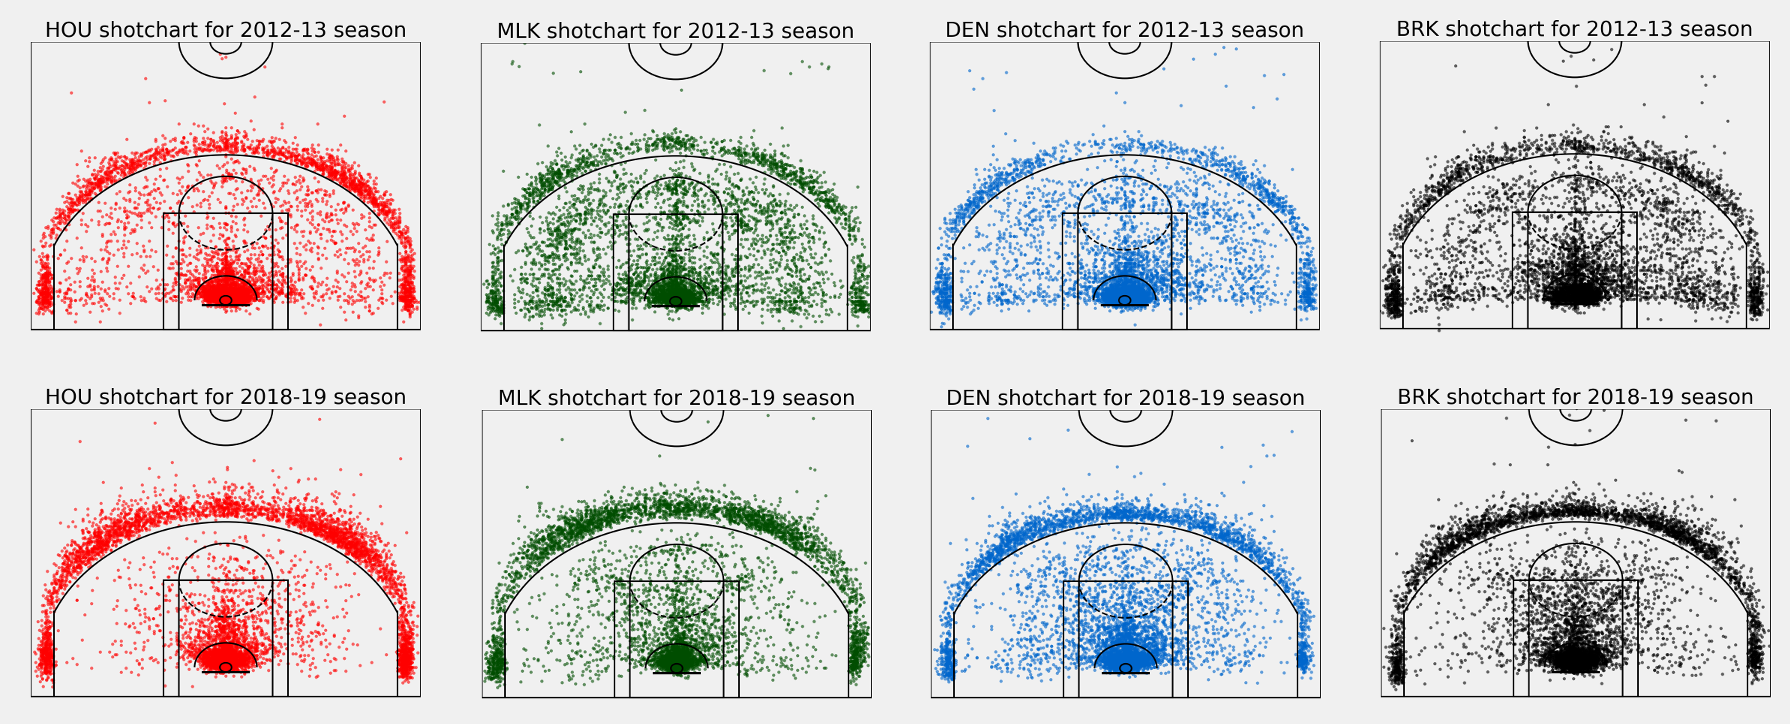
\includegraphics[scale=0.27]{shotcharts.png}
\end{center}
\caption{Shotcharts from 2012-13 and 2018-19 seasons}
\label{plt:shotcharts}
\end{figure}

Team that popularized Moreyball, Houston Rockets, were last in number of mid-range attempts in 2018-19 season. They finished as a 2nd best offense in the league, just 0.4 points per 100 possessions behind 1st ranked Golden State Warriors. They were one of the best offensive teams for a while, finishing top 2 in ORtg in 2016-17 (2nd), 2017-18 (1st) and 2018-19 (2nd) seasons. Not only that, but from the 2012-13 season, they missed top 7 in ORtg only once, in 2014-15 (ranked 12th).

So, Moreyball should work, right? I mean, if a team is shooting just shots that are more efficient than the average, or in other words drastically decrease number of mid-range shots, it will have above average offense. Let's compare ORtg to a percentage of shots that were mid-range, teams took in a 2018-19 season.

\begin{figure}[h!]
\begin{center}
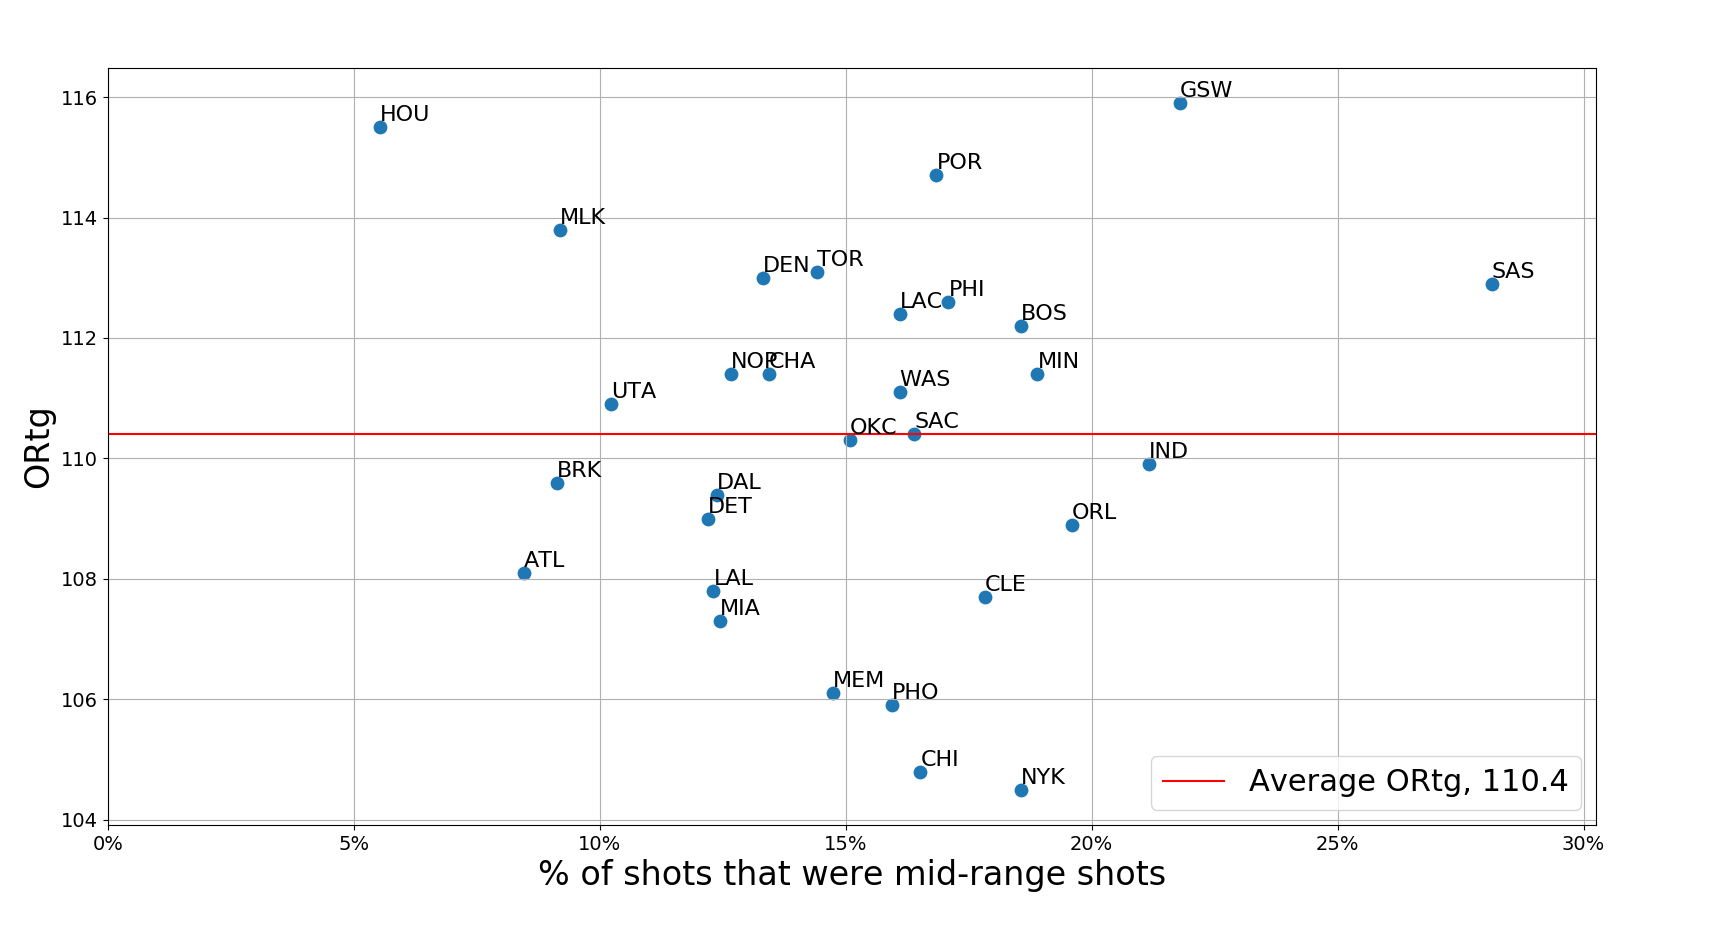
\includegraphics[scale=0.29]{ortg_pct_mid_range.png}
\end{center}
\caption{ORtg to \% of shots that were mid-range by team (2018-19 season)}
\label{plt:ortg_oct_mid_range}
\end{figure}

The results are interesting. Team with the best ORtg, Golden State Warriors, was second in percentage of mid-range shots, while the second-placed Houston was dead last in that category. San Antonio Spurs, team that was first in percentage of mid-range shots, had 7th best offense. Teams such as Atlanta (23rd), Brooklyn (19th) and Milwaukee (4th), besides Houston, had taken less than 10\% of their shots from mid-range, with significant difference in ORtg. So, implementing Morreyball might not produce above average offense, and not only that, but an offense with lot of, usually inefficient, mid-range shots can work well (if a team has efficient mid-range scorer). If that's the case, why would teams even try to play Moreyball?

Because Morreyball leads to a more efficient offense in general! Take a look at table \ref{tab:seasons_comp}. Every season shown has increase of three-point attempt rate from the season before, and with it, better ORtg and better efficiency.

\begin{table}[h!]
\begin{center}
\begin{tabular}{|l|c|c|c|c|c|} \hline
\textbf{Stat \textbackslash Season} & \textbf{2000-01} & \textbf{2005-06} & \textbf{2010-11} & \textbf{2015-16} & \textbf{2018-19} \\ \hline
\textbf{TS\%} & 51.8\% & 53.6\% & 54.1\% & 54.1\% & 56.0\% \\ \hline
\textbf{ORtg} & 103.0 & 106.2 & 107.3 & 106.4 & 110.4 \\ \hline
\textbf{Mid-range attempt freq} & 23\% & 23.6\% & 21.4\% & 16.2\% & 9.2\% \\ \hline
\textbf{3P attempt freq} & 17\% & 20.2\% & 22.2\% & 28.5\% & 35.9\% \\ \hline
\end{tabular}
\caption{Comparing stats through seasons}
\label{tab:seasons_comp}
\end{center}
\end{table}

Correlations on data from season 2000-01 to season 2018-19 (from basketball-reference.com) are showing same results:

\begin{itemize}
	\item Correlation between TS\% and ORtg: 0.967
	\item Correlation between TS\% and \% of 3PA: 0.851
	\item Correlation between TS\% and \% of mid-range attempts: -0.733
	\item Correlation between \% of 3PA and ORtg: 0.766
	\item Correlation between \% of mid-range attempts and ORtg: -0.634
\end{itemize}

Results are, based on everything we have seen so far, expected. There is a very strong correlation between efficiency and ORtg. True shooting percentage depends more on frequency of 3-point shots than on frequency of mid-range shots. More three-pointers, better efficiency, but also fewer mid-range shots, better efficiency, just not to the same degree. These are just some extra reasons why Moreyball does produce more points per possession!

To conclude, Moreyball produces more points per possession in general, but offenses that are more Moreyball than the others might not be above average on a season level. Rise in Moreyball contributed to the rise in ORtg in recent years. Also, let's note that strategies with lot of mid-range shooting can produce good/above average offense. % maybe why?


\section{Clustering}
\label{sec:clustering}

In this section I will try to, via clustering, find interesting things in NBA data. Clustering is process of finding different groups in data, where element in one group is more similar to another element in the same group than to any element from any other group \cite{clustering}. Those groups are called \textbf{clusters}. Following algorithms will be used.

First one is \textbf{K-Means clustering.} This algorithm will find \textbf{K} groups. Every group will be represented by one point, called \textit{centroid}. Point that is not a centroid will belong to the cluster that is represented by it's closest centroid. Algorithm will first choose K centroids at random, and then perform iterative calculations to optimize positions of mentioned centroids. User can choose number of iterations. Because centroids are initialized at random, algorithm should be executed muliple times. Then, out of all results, the best one is selected. \cite{clustering}

Second is \textbf{Hierarchical clustering.} There are two types, \textbf{divisive} and \textbf{agglomerative} clustering. Former method begins with one cluster that contains every data point. Then, iteration by iteration, it will split that cluster in smaller ones, by similarity, until every point is cluster for itself. Latter is the opposite. It will start with as many clusters as data points, and then it will, iteratively, group two that are the most similar into one group, until only one cluster, that contains every data point, remains. \cite{clustering}

Similarity between clusters is calculated by \textbf{linkage}. In \textit{single} linkage, the smaller the distance between closest points of two clusters is, the more similar they are. \textit{Complete} linkage is the opposite, it takes into account distance between the furthest points of two clusters. The closer they are the similarity between clusters is greater. \textit{Average} linkage takes into account average distance from any point that belongs to one cluster to any point that belongs to the other cluster. The smaller the distance, the more similar they are. The last one is \textit{Ward's} linkage. Similar to previous one, but instead of average, it calculates sum of squared distances. \cite{clustering}\cite{hierarchical}

One of the metrics that can tell if the clustering is good or not is \textbf{silhouette score}, calculated, for data point in cluster, as $ (b - a)  / max(a, b) $, where \textit{a} is average distance to other data point in the same cluster, \textit{b} is average distance to other data point in the nearest cluster. Values for this score can go from -1 to 1. The higher value the better clustering. In other words, silhouette score measures how similar a data point in a cluster is similar to its own cluster compared to other clusters by comparing the point’s distance from its own cluster to its distance from other clusters. \cite{clustering}

\subsection{Determining players' roles by games played}
\label{subsec:players_roles}

Player in the NBA can usually be placed in one of the three categories, starter, bench player and non-rotational player. First group, starters, are expected to start every game they play. Starters play the most minutes per game. They might not play every game due to various injuries and rest days. Also, they might not start every game. For example, starter might get injured, and when he is healed coach might not put him in the starting lineup. That is usually practice if the starter is on a minute restriction, meaning he will play in the game, but will play in the fewer minutes than he usually plays in when he starts. Second group are bench players. They are not usually starters, but are important for the success of the team. They play in a lot of minutes, but not as much as starters. Bench players might get to start some games because starter is injured, or maybe because of matchups, but that is not really likely. Third are non-rotational players. They aren't usually playing in the game, or if they are, they are playing small amount of minutes or garbage time. Note that these players also might even start some games, if team has serious problem with injuries. Also, it's possible that a player makes progress or regress during a season, which will result in promotion or demotion.

The starting point is clustering based on games played (\textbf{G}) and games started (\textbf{GS}). It is expected that players with small amount of games are the non-rotational ones, the ones that started lot of games are starters and the others are bench players. Data is shown on figure \ref{plt:g_gs} and represents players from 2018-19 season. I believe that the biggest difference between results of clustering algorithms will be in the area in the middle of the diagonal, where players did start every (or almost every) game they played in, but maybe didn't play enough games to be considered starters.

\begin{figure}[h!]
\begin{center}
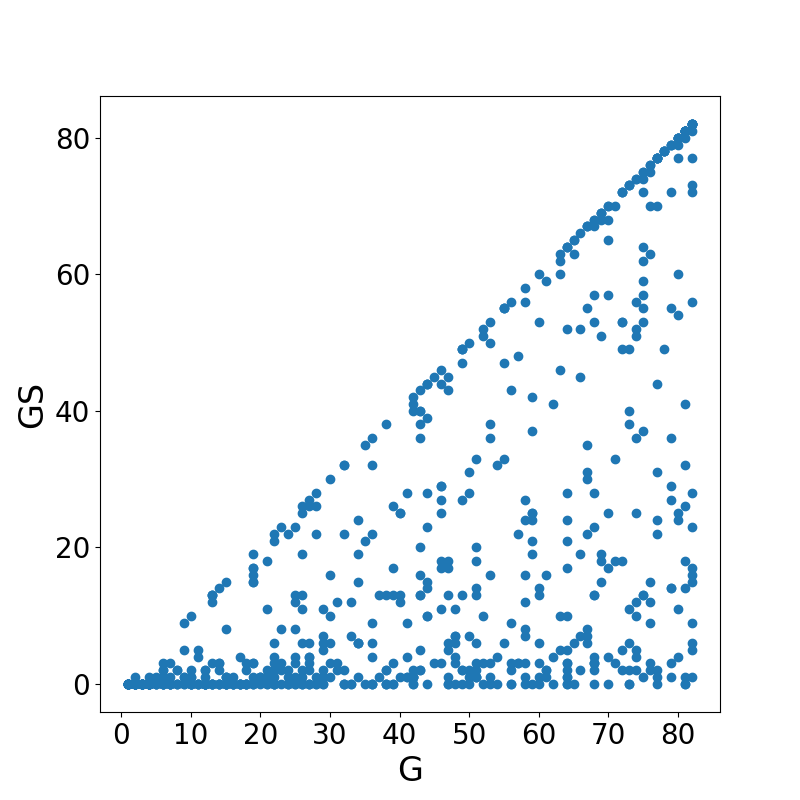
\includegraphics[scale=0.3]{g_to_gs.png}
\end{center}
\caption{Games played to Games started (2018-19 season)}
\label{plt:g_gs}
\end{figure}

The first clustering algorithm is K-Means. Value of K is 3 because players are supposed to be grouped in three groups. After that, I tried hierarchical clustering methods with simple, complete, average and Ward's linkage. Results can be found in table \ref{tab:clust_score_k3}.

\begin{table}[!h]
\begin{center}
\begin{tabular}{|l|c|} \hline
\textbf{Clustering method} & \textbf{Silhouette score}  \\ \hline
K-Means & 0.550  \\ \hline
Hierarchichal, simple linkage & -0.007  \\ \hline
Hierarchichal, complete linkage & 0.524  \\ \hline
Hierarchichal, average linkage &  0.519  \\ \hline
Hierarchichal, Ward's linkage & 0.495  \\ \hline
\end{tabular}
\caption{Silhoutte score for G and GS}
\label{tab:clust_score_k3}
\end{center}
\end{table}

Judging by the silhouette score, clusters aren't well defined, which could also be assumed from the previous plot. Method with the best score is K-Means.
Let's take a look at the results (figure \ref{plt:clust_g_gs_k3}).

\begin{figure}
\centering
\begin{minipage}{.22\textwidth}
  \centering
  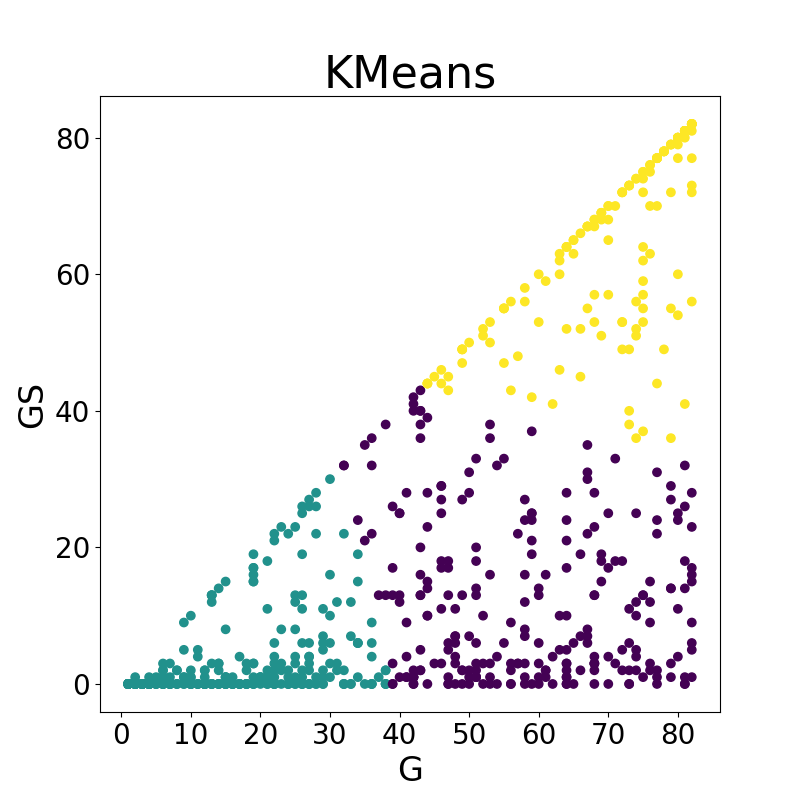
\includegraphics[scale=0.14]{kmeans_g_gs.png}
  \label{fig:kmeans_g_gs}
\end{minipage}
\begin{minipage}{.22\textwidth}
  \centering
  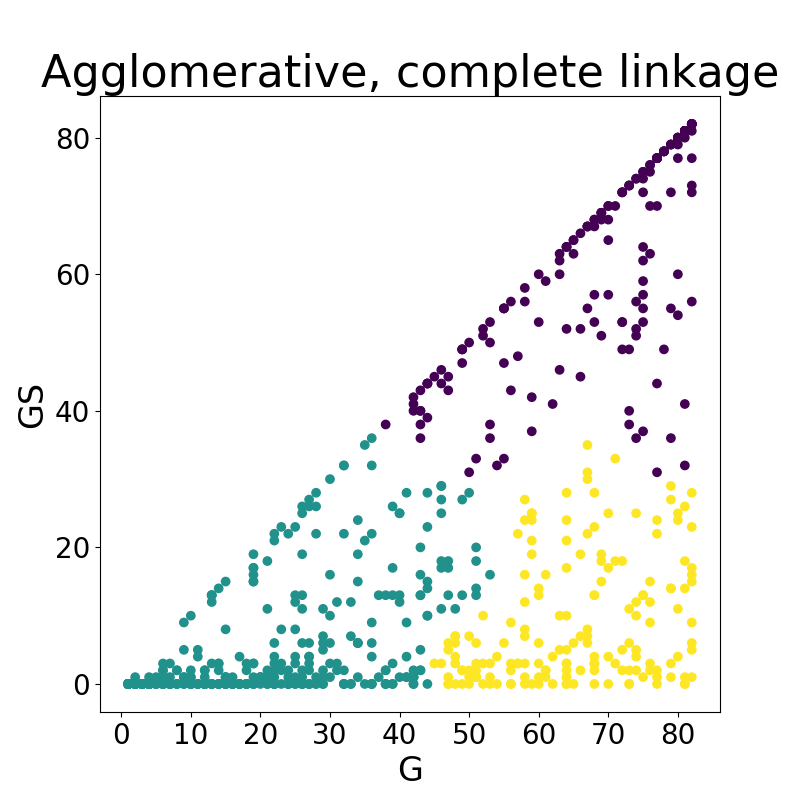
\includegraphics[scale=0.14]{complete_link_g_gs.png}
  \label{fig:complete_g_gs}
\end{minipage}
\begin{minipage}{.22\textwidth}
  \centering
  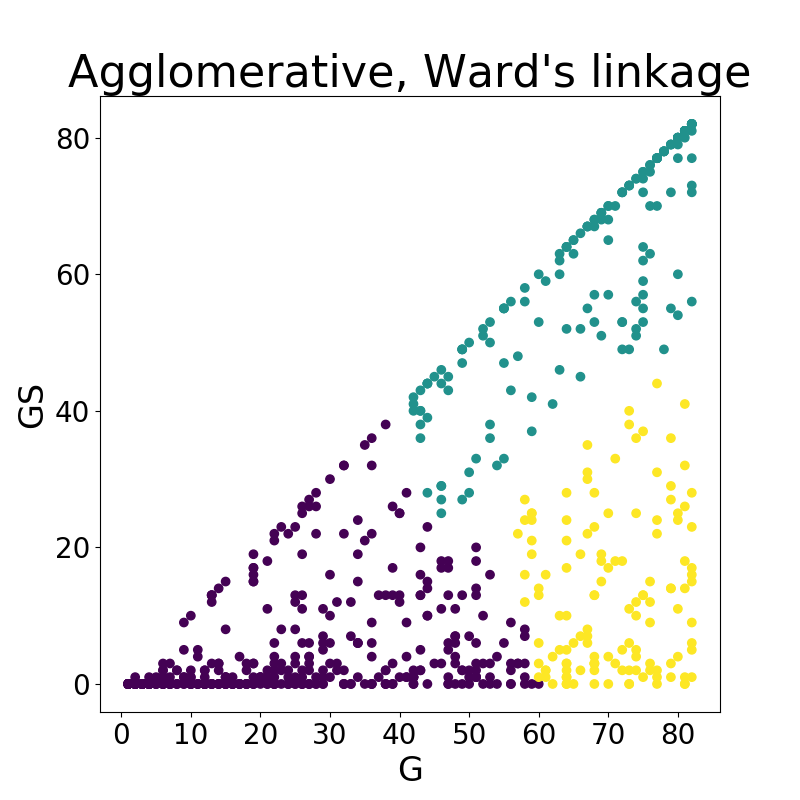
\includegraphics[scale=0.14]{ward_link_g_gs.png}
  \label{fig:ward_g_gs}
\end{minipage}
\begin{minipage}{.22\textwidth}
  \centering
  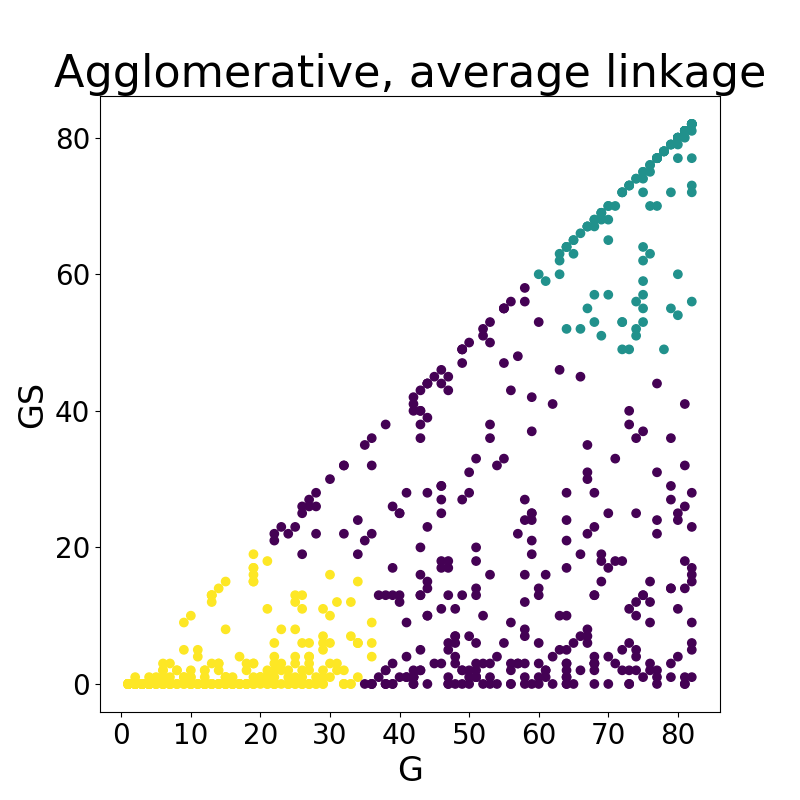
\includegraphics[scale=0.14]{average_link_g_gs.png}
  \label{fig:average_g_gs}
\end{minipage}
\caption{Clusters on G and GS data}
\label{plt:clust_g_gs_k3}
\end{figure}

The results are somewhat expected. In the upper right corner is the cluster that contains starters. In the lower left are players that are outside of rotation while bench players are in between. Clustering  with K-Means and agglomerative with average linkage is somewhat similar, where players in the middle of the diagonal are considered bench players. In the other two, those players are starters.

Maybe the clustering will have better results if we add one more variable, minutes played (\textbf{MP}). It is expected that starters play the most minutes per game, while players that are outside of rotation play the least, if any. Bench players should play, but not as much as starters. Also, note that values of MP per game, for 2018-19 season, are between 0 and 36.9, the amount of minutes the league leaders, Bradley Beal and Paul George, played per game. Values of G and GS are from 0 to 82. Because of that, it is possible that normalizing data (scaling to [0, 1] interval) before clustering might improve results. Scaling data means that difference of one minute played per game won't have the same significance as difference of one game played.

As we have already seen, because of the data, clusters cannot really be well defined, so the part with silhouette score is skipped. Results for non-scaled data are shown in the figure \ref{plt:clust_g_gs_mp_k3} while results for scaled data are in figure \ref{plt:clust_g_gs_mp_k3_scaled}. Note that clusters are still shown in G to GS plot, even with MP variable included in clustering. The reason behind this is comparing results with the previous one.

\begin{figure}
\centering
\begin{minipage}{.22\textwidth}
  \centering
  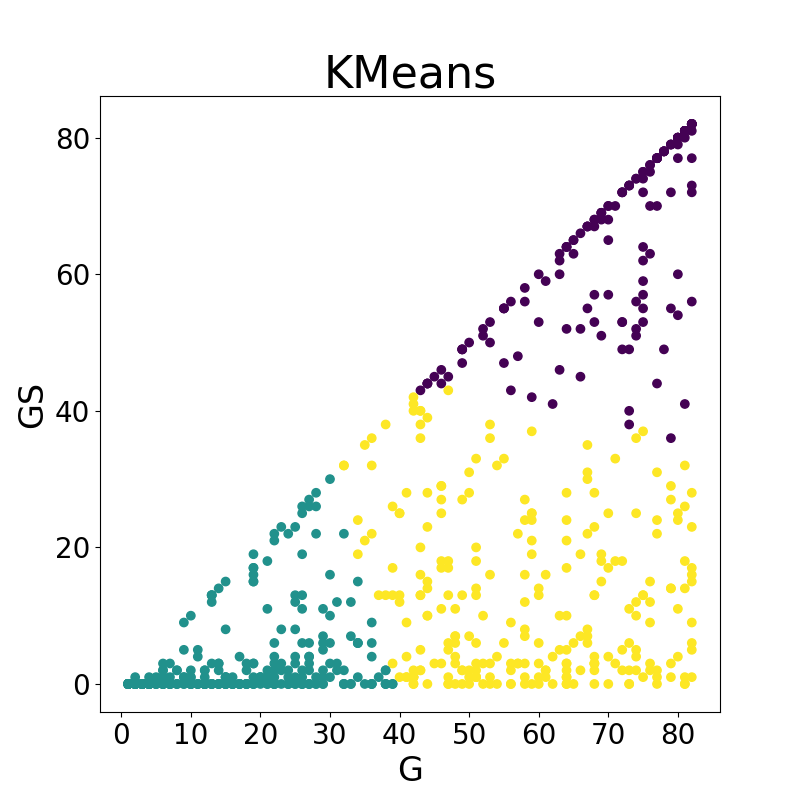
\includegraphics[scale=0.14]{kmeans_g_gs_mp.png}
  \label{fig:kmeans_g_gs_mp}
\end{minipage}
\begin{minipage}{.22\textwidth}
  \centering
  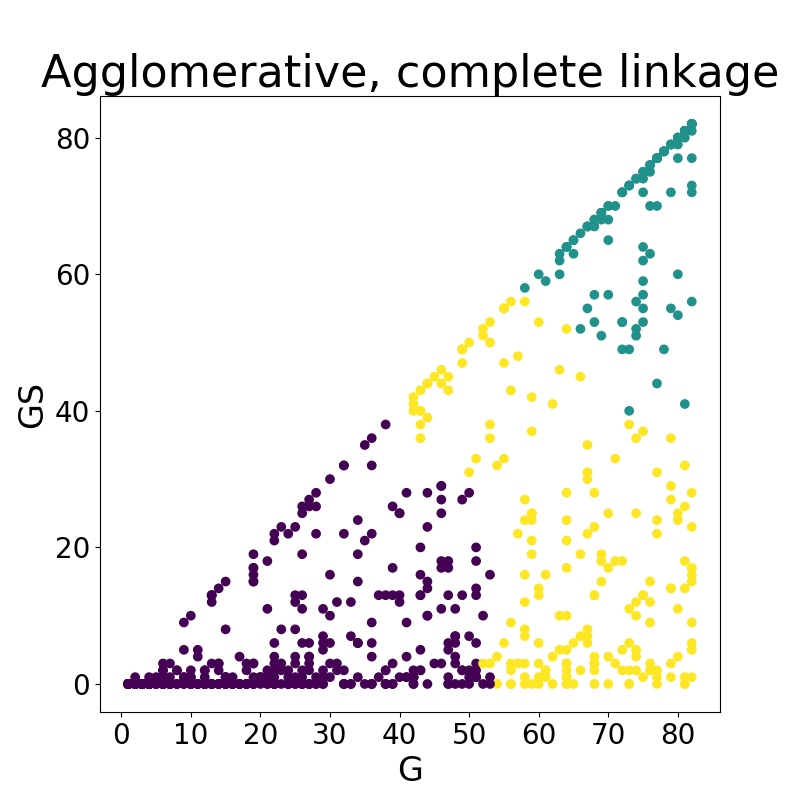
\includegraphics[scale=0.14]{complete_link_g_gs_mp.png}
  \label{fig:complete_g_gs_mp}
\end{minipage}
\begin{minipage}{.22\textwidth}
  \centering
  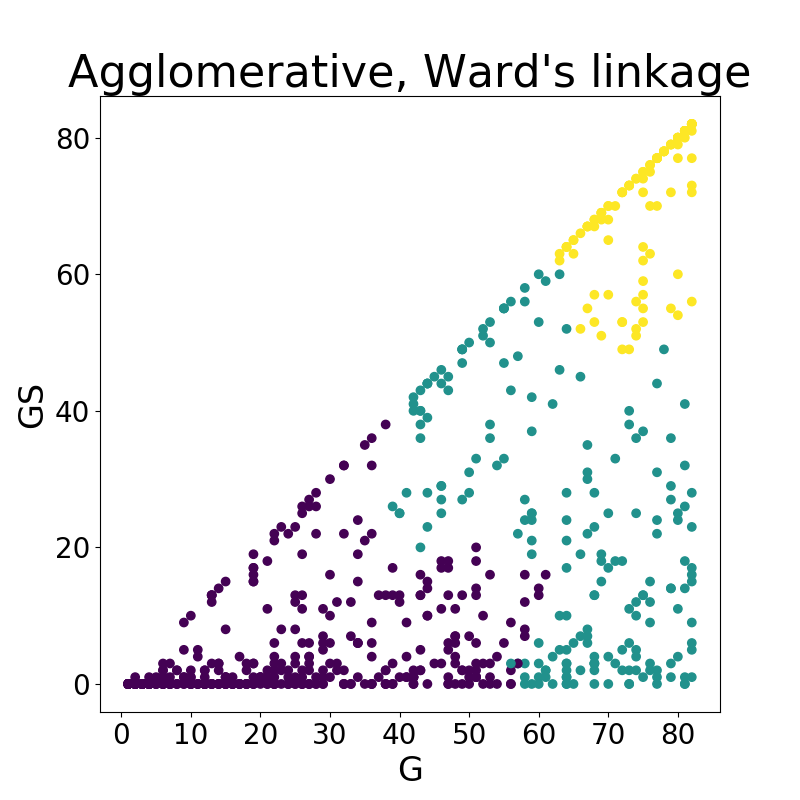
\includegraphics[scale=0.14]{ward_link_g_gs_mp.png}
  \label{fig:ward_g_gs_mp}
\end{minipage}
\begin{minipage}{.22\textwidth}
  \centering
  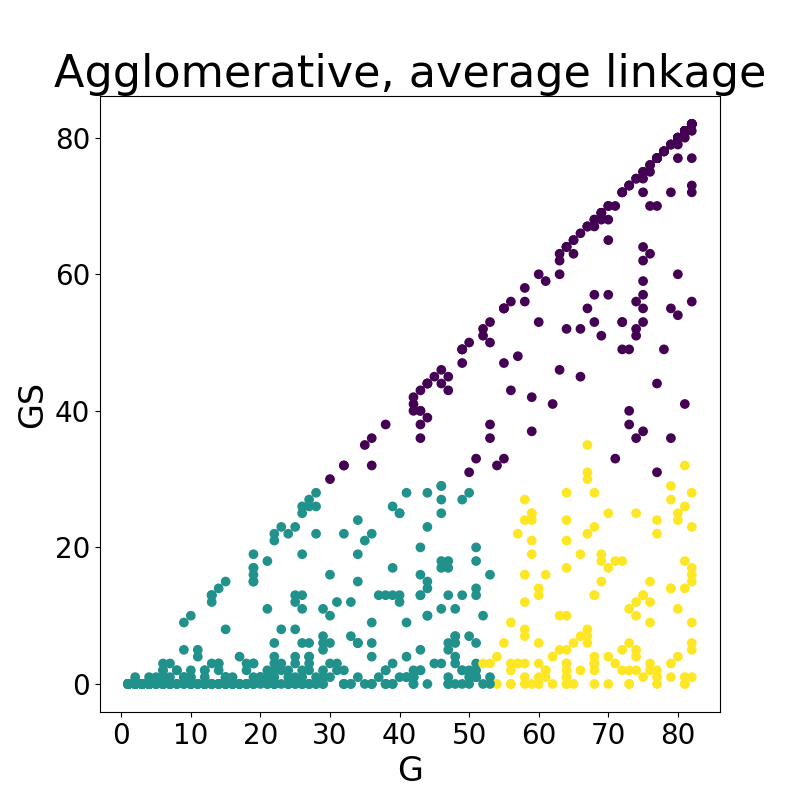
\includegraphics[scale=0.14]{average_link_g_gs_mp.png}
  \label{fig:average_g_gs_mp}
\end{minipage}
\caption{Clusters on G, GS and MP data}
\label{plt:clust_g_gs_mp_k3}
\end{figure}

K-Means algorithm have almost the same results as before, while others are different. The main difference is, unsurprisingly, middle of the diagonal. As opposed to before, agglomerative with complete and Ward's linkage are grouping it with bench players. Agglomerative with average linkage changed the most, with middle of the diagonal in starters group. Clustering on scaled data will probably give different results (figure \ref{plt:clust_g_gs_mp_k3_scaled}).

\begin{figure}
\centering
\begin{minipage}{.22\textwidth}
  \centering
  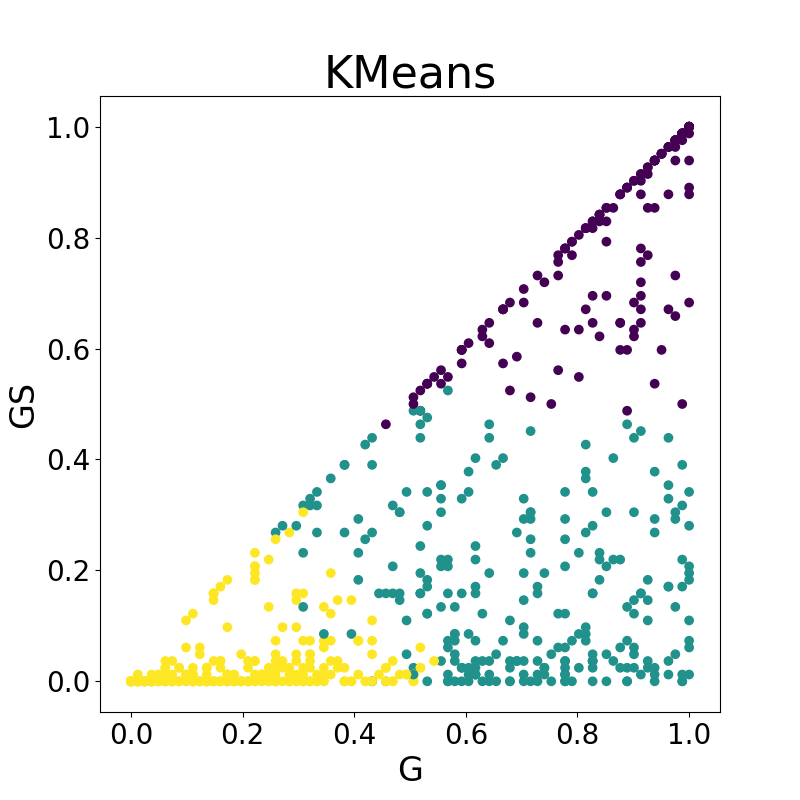
\includegraphics[scale=0.14]{kmeans_g_gs_mp_scaled.png}
  \label{fig:kmeans_g_gs_mp_scaled}
\end{minipage}
\begin{minipage}{.22\textwidth}
  \centering
  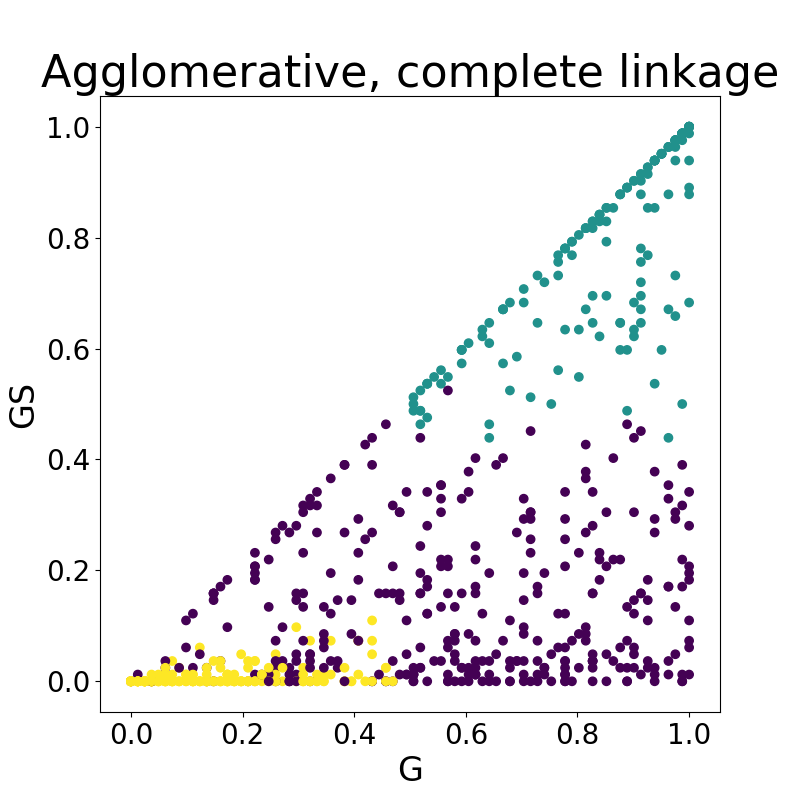
\includegraphics[scale=0.14]{complete_link_g_gs_mp_scaled.png}
  \label{fig:complete_g_gs_mp_scaled}
\end{minipage}
\begin{minipage}{.22\textwidth}
  \centering
  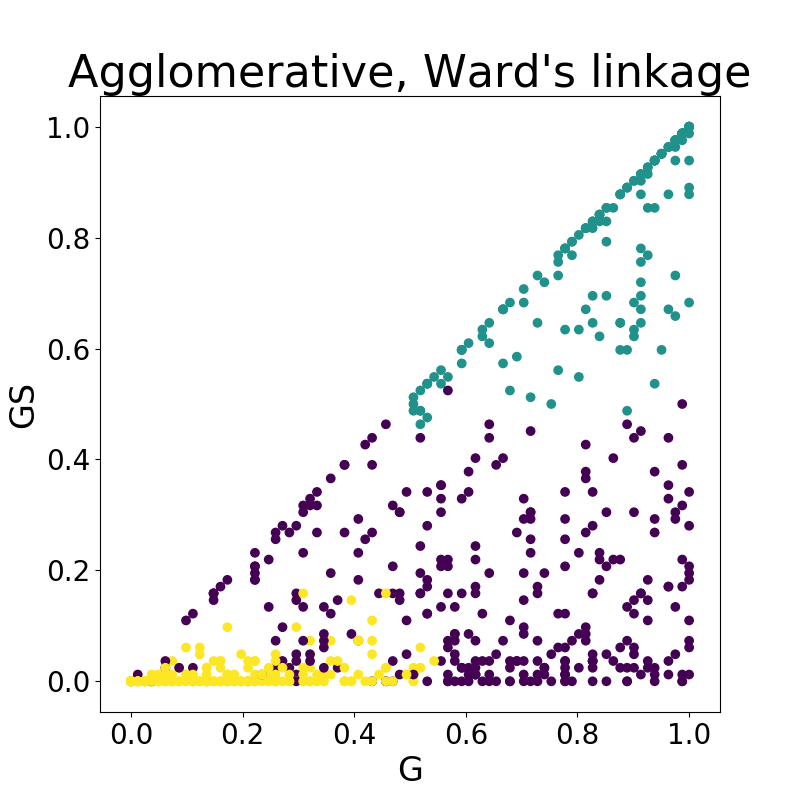
\includegraphics[scale=0.14]{ward_link_g_gs_mp_scaled.png}
  \label{fig:ward_g_gs_mp_scaled}
\end{minipage}
\begin{minipage}{.22\textwidth}
  \centering
  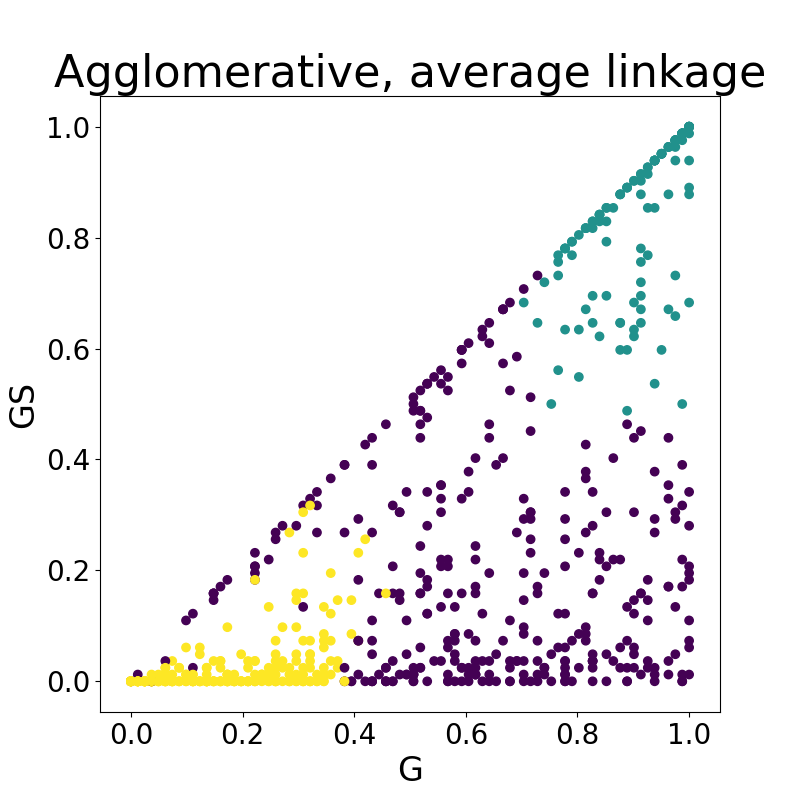
\includegraphics[scale=0.14]{average_link_g_gs_mp_scaled.png}
  \label{fig:average_g_gs_mp_scaled}
\end{minipage}
\caption{Clusters G, GS and MP, scaled data}
\label{plt:clust_g_gs_mp_k3_scaled}
\end{figure}

Scaling data definitely gave us different results, although results from K-Means are still similar to the previous ones. The biggest difference can be observed in cluster with non-rotational players. Players in that cluster played at most somewhere around half of the games, but did not start in almost any of them. Because of that, cluster with bench players increased in size. Cluster with starters remained somewhat same.

Clusters with starters were upper right, clusters with non-rotational players were lower left, and clusters with bench players were lower right, as expected. There were different results in clustering of the middle of the diagonal, that usually belonged with the starters or bench players. There is a case to be made for both, but I am personally more leaning towards starters option. That part of the diagonal contains players that played somewhere between 40 and 55 games, and started in a lot of them (or almost all of them). Notable players from that group are LeBron James, Brandon Ingram, Wayne Ellington, Wendell Carter, Lonzo Ball, Tristan Thompson, Will Barton etc. I would personally count them as starters, who missed significant part of the season due to injuries or other reasons. I like results of agglomerative clustering with Ward's linkage on games and games started data, although I would argue that more players from non-rotational players cluster should belong to the bench cluster, specifically the ones that played more than 40 games.

\subsection{Clustering shooters}
\label{subsec:clust_shooters}

In basketball, shooting is the most important aspect of the game (or scoring, rather, but you must shoot to score), and different players are shooting from different places on the court, called zones. Some of them are good at three point shooting while others, although mostly centers, are shooting most of their shots near the basket. The area from which players shoot is important, as we have seen in the Moreyball section (number \ref{sec:moreyball}). In this section, I will try to group players based on shooting from previously mentioned zones.

\subsubsection{Data}
\label{subsubsec:clust_shooters_data}

First, let's talk about data used. Data (from stats.nba.com) contains shooting attempts from 2018-19 season (totals, not per game) from various zones for every player that shot more than 300 shots in a season. Those zones are:

\begin{itemize}
	\item \textbf{Restricted area} - Area four feet from the basket. It is denoted by an arc inside the paint.
	\item \textbf{In the paint (non-restricted area)} - Area between restricted area, and mid-range (from 3 to 10 ft. from the basket).
	\item \textbf{Mid-range} - Shots from somewhere between 10 feet and the three point line.
	\item \textbf{Corner three} - Three point shot taken from the left or right corner.
	\item \textbf{Above the break three} - Every three pointer that isn't taken from one of the corners. 
\end{itemize}

\subsubsection{Determining optimal number of clusters}
\label{subsubsec:clust_shooters_num_of_clusters}

Algorithm used for clustering is K-Means. In the previous section, number of clusters was known, three, because I wanted to group players into three different roles. For this problem, that number is unknown, so first thing that must be done is to determine an optimal number of clusters in the data. To do that I used silhouette scores. In the figure \ref{plt:num_cls_shooting} values for silhouette scores for different number of clusters are shown. 

\begin{figure}[h!]
\begin{center}
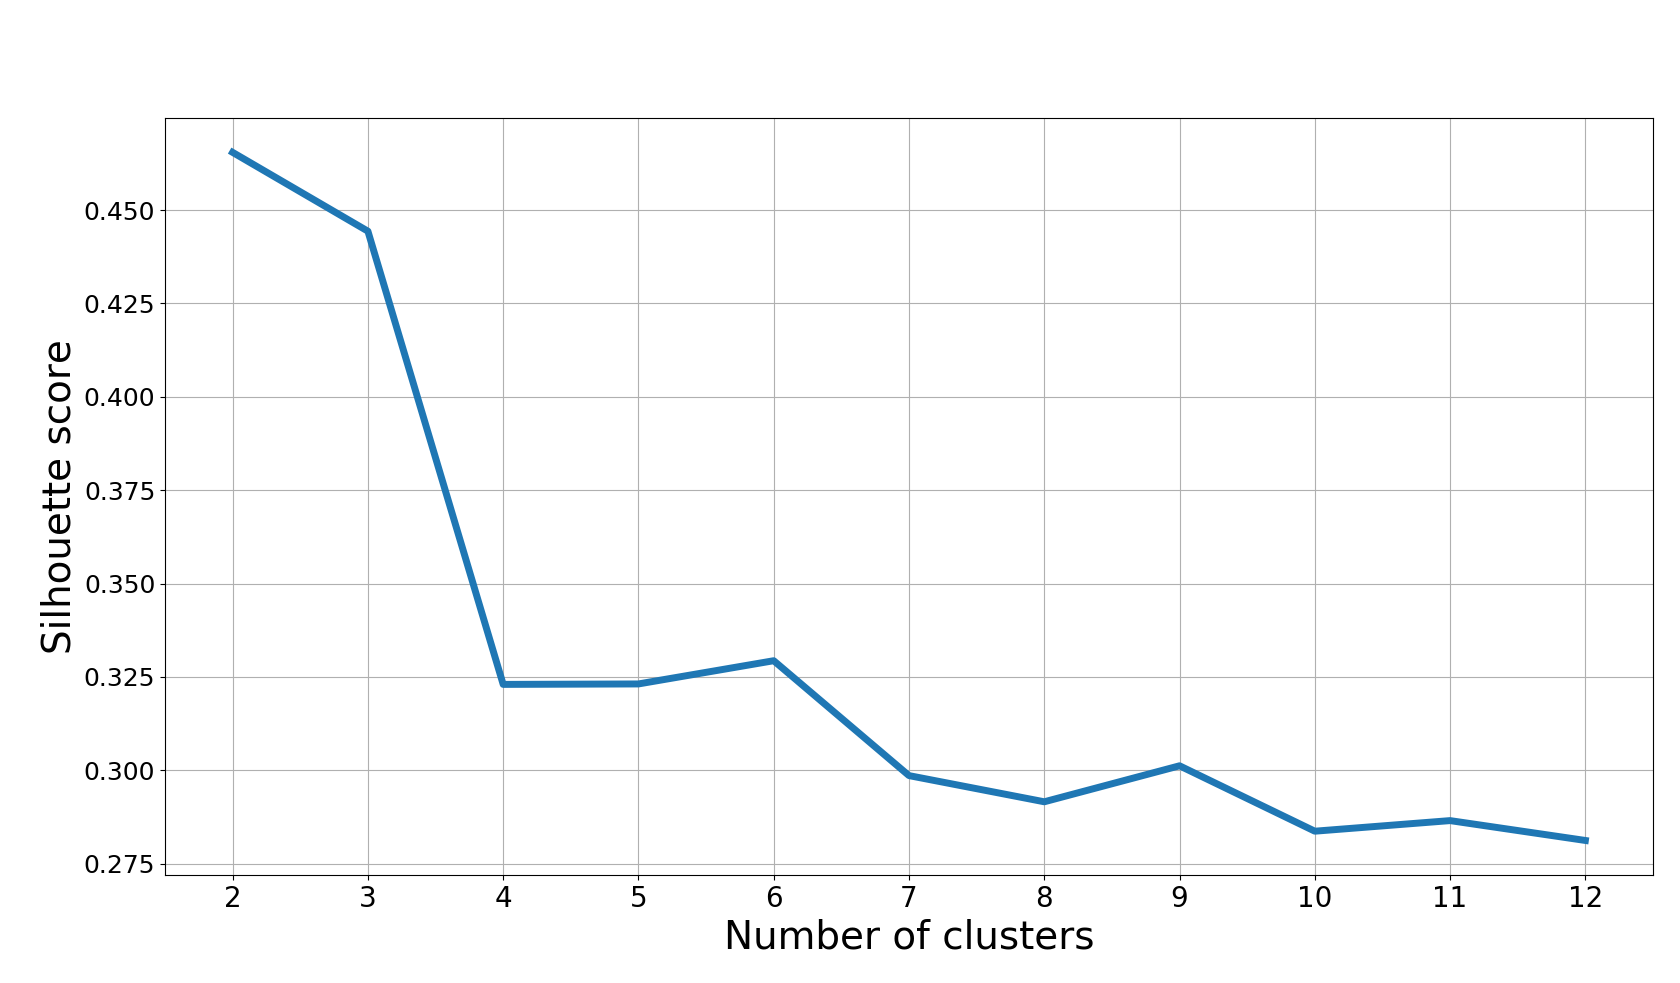
\includegraphics[scale=0.28]{num_of_clusters_shooting.png}
\end{center}
\caption{Silhouette score for different number of clusters}
\label{plt:num_cls_shooting}
\end{figure}

This is expected because, usually, silhouette score decreases as number of clusters increases. But, that does not mean that we will use two clusters to represent data, because that number of clusters does not give any information about it. Instead of looking at value of silhouette scores, we will look at their difference, but not difference by subtraction, but difference based on how many percent did silhouette score change from \textbf{k number} of clusters to \textbf{k+1 number} of clusters. That difference is calculated as $ 1 - ((1 - v) / (1 - w)) $ where v is silhouette score for x number of clusters and w is silhouette score for x-1 number of clusters. Plot is shown on figure \ref{plt:num_cls_pct_change}.

\begin{figure}[h!]
\begin{center}
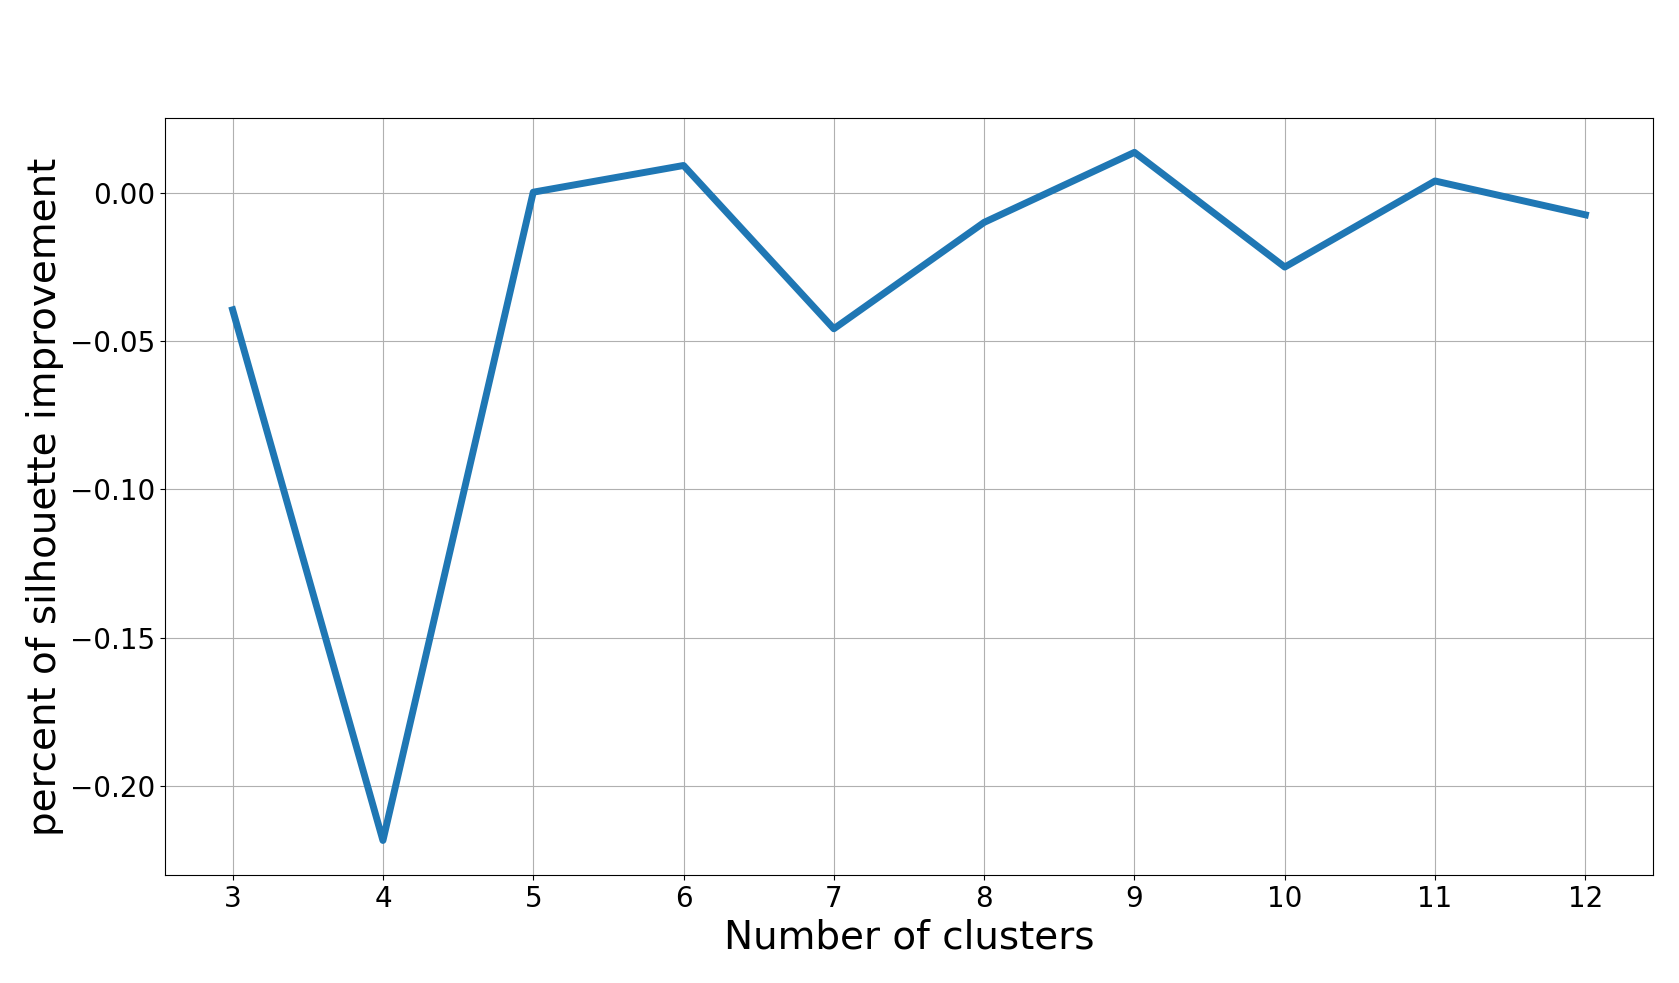
\includegraphics[scale=0.28]{num_of_clusters_shooting_pct_change.png}
\end{center}
\caption{Percentage of changes of silhouette scores}
\label{plt:num_cls_pct_change}
\end{figure}

To select optimal number of clusters, we will just select the ones with the greatest positive improvement. The highest scores are for five, seven and nine clusters, but the one for K-Means with nine clusters is higher than others, so that is the one that will be used.

\subsubsection{Results}
\label{subsubsec:clust_shooters_results}

As mentioned before, algorithm is K-Means and number of cluster is set to nine. Every cluster will have it's name based on either playstyle or zone players inside it shot most of their shots from. Following clusters are created:


\begin{enumerate}
	\item \textbf{Low volume shooters. Bad offensive players}; 93 players: Avery Bradley, Waiters, Draymond Green, Jonas Jerebko, Isaac, Dunn, Hezonja, Seth Curry etc.
	\item \textbf{Medium volume shooters. Players that probably weren't focal point of the offense}:  30 players: Horford, Portis, Rose, Garry Harris, Jaylen Brown, Turner, Rubio, Gay etc.
	\item \textbf{High volume shooters. Players that can score from everywhere and were focal point of the offense}; 18 players: Davis, Griffin, Embiid, LeBron, Jokić, Westbrook, Tobias Harris, Trae Young, LaVine etc.
	\item \textbf{Lower volume good distance shooters}; 44 players: Rivers, Bogdan Bogdanović, Paul, Eric Gordon, VanVleet, Crowder, Ingles, Ariza etc.
	\item \textbf{Higher volume good distance shooters. They were also good inside the three-point line}; 27 players: McCollum, Gallinari, Booker, Redick, Durant, Irving, Klay Thompson, Marc Gasol etc.
	\item \textbf{Lower volume bad distance shooters}; 33 players: Adebayo, DeAndre Jordan, Powell, Zubac, Okafor, Looney, Plumlee, Robin Lopez etc.
	\item \textbf{Higher volume bad distance shooters}; 19 players: Drummond, Ben Simmons, Capela, Giannis, Randle, Siakam, Gobert, Adams etc.
	\item \textbf{Three Point Gods. Players who shot a lot of three-pointers, but were also very good in RA}; 8 players: Beal, Hield, D'Angelo Russell, Lillard, Harden, Walker, Paul George, Steph Curry 
	\item \textbf{SA Spurs All-stars. Mid-range players}; 2 players: LaMarcus Aldridge and DeMar DeRozan
\end{enumerate}

Information about how many shots by zone did average player attempted by cluster, or in other words centroids generated by K-Means, can be found in the table \ref{tab:avg_by_clst}.

\begin{table}[!h]
\begin{center}
\begin{tabular}{|c|c|c|c|c|c|} \hline
Cluster & RA & Paint non-ra & Mid-range & Corner 3 & Above the break 3 \\ \hline
1 & 125.14 &  65.6 & 68.6 &  55.2 & 139.0 \\ \hline
2 & 253.8 & 129.1 & 140.5 & 53.1 & 151.9 \\ \hline
3 & 427.9 & 231.2 & 187.6 &  49.0 & 302.6 \\ \hline
4 & 137.3 & 72.9 & 78.5 & 86.4 & 295.7 \\ \hline
5 & 253.0 & 185.1 & 256.6 & 61.1 & 353.9 \\ \hline
6 & 250.2 & 92.2 & 32.9 & 21.7 & 43.5 \\ \hline
7 & 536.8 & 171.8 & 63.9 & 19.8 & 38.8 \\ \hline
8 & 389.0 & 190.25 & 260.1 & 84.8 & 641.9 \\ \hline
9 & 365.0 & 345.0 & 562.5 & 13.0 & 30.0 \\ \hline
\end{tabular}
\caption{Average attempts from zone by cluster}
\label{tab:avg_by_clst}
\end{center}
\end{table}

These results are very interesting. First, note that already mentioned mid-range centered offense of San Antonio Spurs produced one cluster, containing only two players, DeRozan and Aldridge, who barely shot any three-pointers. There is a cluster with players that just didn't shot much, containing some either not good offensive players, players that came from the bench or some players that were injured during the season and didn't menage to shoot as many times as some other players from different clusters. There are two clusters with players that specialized in three-point shooting, clusters 4 and 5. Cluster four mostly consists of shooting guards, wings and some stretch fours. That cluster also contains Brook Lopez, who shot around 510 threes in a season, way more than the average for that cluster. Reason behind that is his small number of restricted area attempts. Cluster number five contains mostly guards and some wings, but also Marc Gasol, center, which is interesting.  Centers from cluster six are mostly not offensively talented, or not talented at all, because they didn't play much. Cluster number seven contains good players, but bad distance shooters, mostly centers, but also Ben Simmons and 2018-19 MVP, Giannis Antetokounmpo. Players that can score from anywhere on the court can be found in cluster number three. A lot of these players are All-stars, All-NBA players or players with a potential to become one. There is  also cluster eight, cluster with players that shot massive amount of three pointers, but are also good from everywhere else. Definitely a good company to be in.

In the end, let's note that these clusters could be a little bit misleading. First, data takes into account only attempts, not makes, so a player that shoots a lot of threes, but at low percentage, might be in the same group as other players who are good or very good three-point shooters. Also, data represents totals in season, not per game stats! Because of that, player that missed significant portion of the season might be in the wrong group. For example, player shot five three-pointers per game, which should put him in the cluster number five if he played in 82 games. But if he missed, let's say, half of the season, his per game stats stay the same, but his total stats take a hit and because of that he might end up in the cluster number four.

\subsection{Clustering shooting by teams}
\label{subsec:clust_shooting_by_teams}

In this decade (2010's), players started to exclude mid-range from their games in favor of more efficient three-point shots and shots that are closer to the basket. But that change did not happen overnight, it took several seasons. Also, some teams adopted that approach before the others. In this section, I will group teams from 2010's into groups based on the area they were shooting from.

It is expected that teams from the same season have similar shot distribution and thus might be in the same group. This will maybe allow us to see the process of elimination of the mid-range across seasons. Also, this might show us shot distributions that were outdated, or before their time, for the season they were used in. For example, if there is an offense from 2018-19 season that shot from the same places on the court as, let's say twenty offenses from 2012-13, we will know that that offense was outdated. Of course, that does not mean it didn't work in 2018-19, but it would mean that most of the teams from that season preferred to score from other spots on the court.

\subsubsection{Data}
\label{subsubsec:clust_shooting_by_teams_data}

Data contains shooting attempts per game from four zones on the court for every team from 2010-11 to 2018-19 season, nine seasons total. Those zones are Restricted area, Paint (non-restricted area), Mid-range and Three-point line (above the break and corner three-pointers are combined).

\subsubsection{Determining optimal number of clusters}
\label{subsubsec:clust_shooting_by_teams_num_of_clusters}

Algorithm used for clustering is K-Means, but K is unknown. Same process for finding optimal value of K will be used as in the previous section. First, we will check silhouette scores for different values of K (figure \ref{plt:clust_shooting_by_teams_plot1}) and then, we will take a look at the precentage of improvement from K clusters to K+1 clusters (figure \ref{plt:clust_shooting_by_teams_plot2}). After that, the best result is selected.

\begin{figure}[h!]
\begin{center}
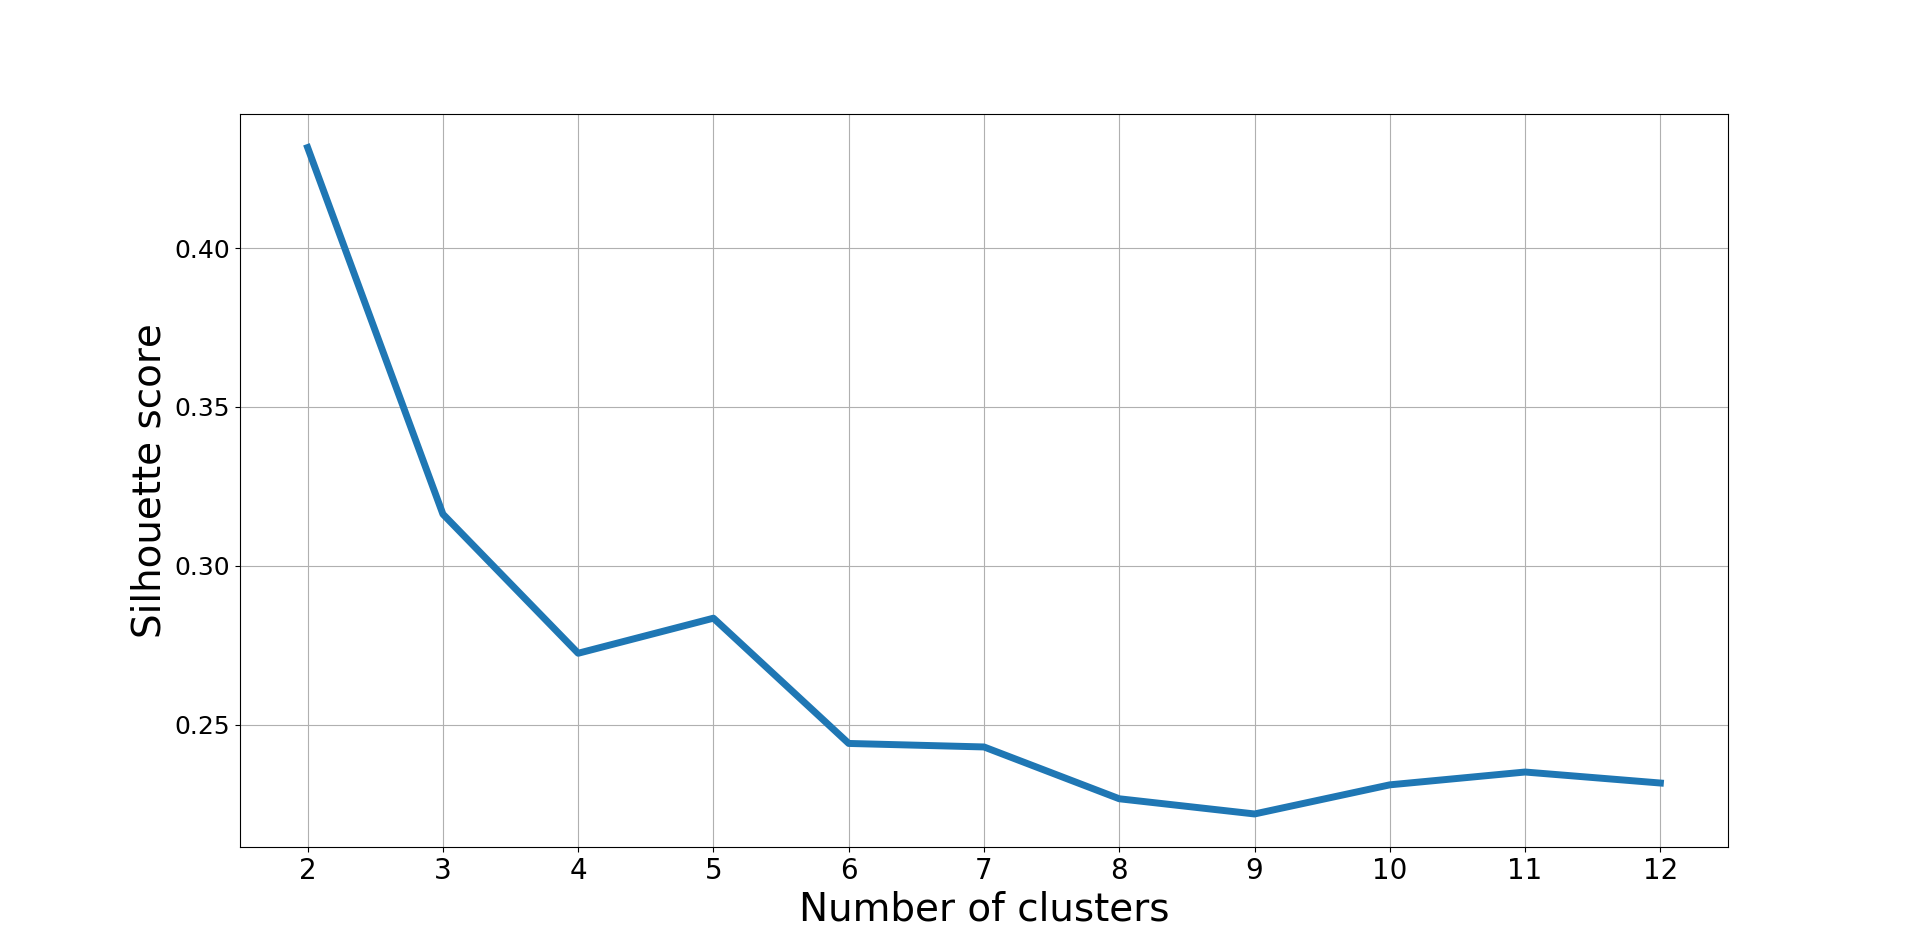
\includegraphics[scale=0.28]{num_of_clust_teams_shooting.png}
\end{center}
\caption{Silhouette score for different number of clusters}
\label{plt:clust_shooting_by_teams_plot1}
\end{figure}

\begin{figure}[h!]
\begin{center}
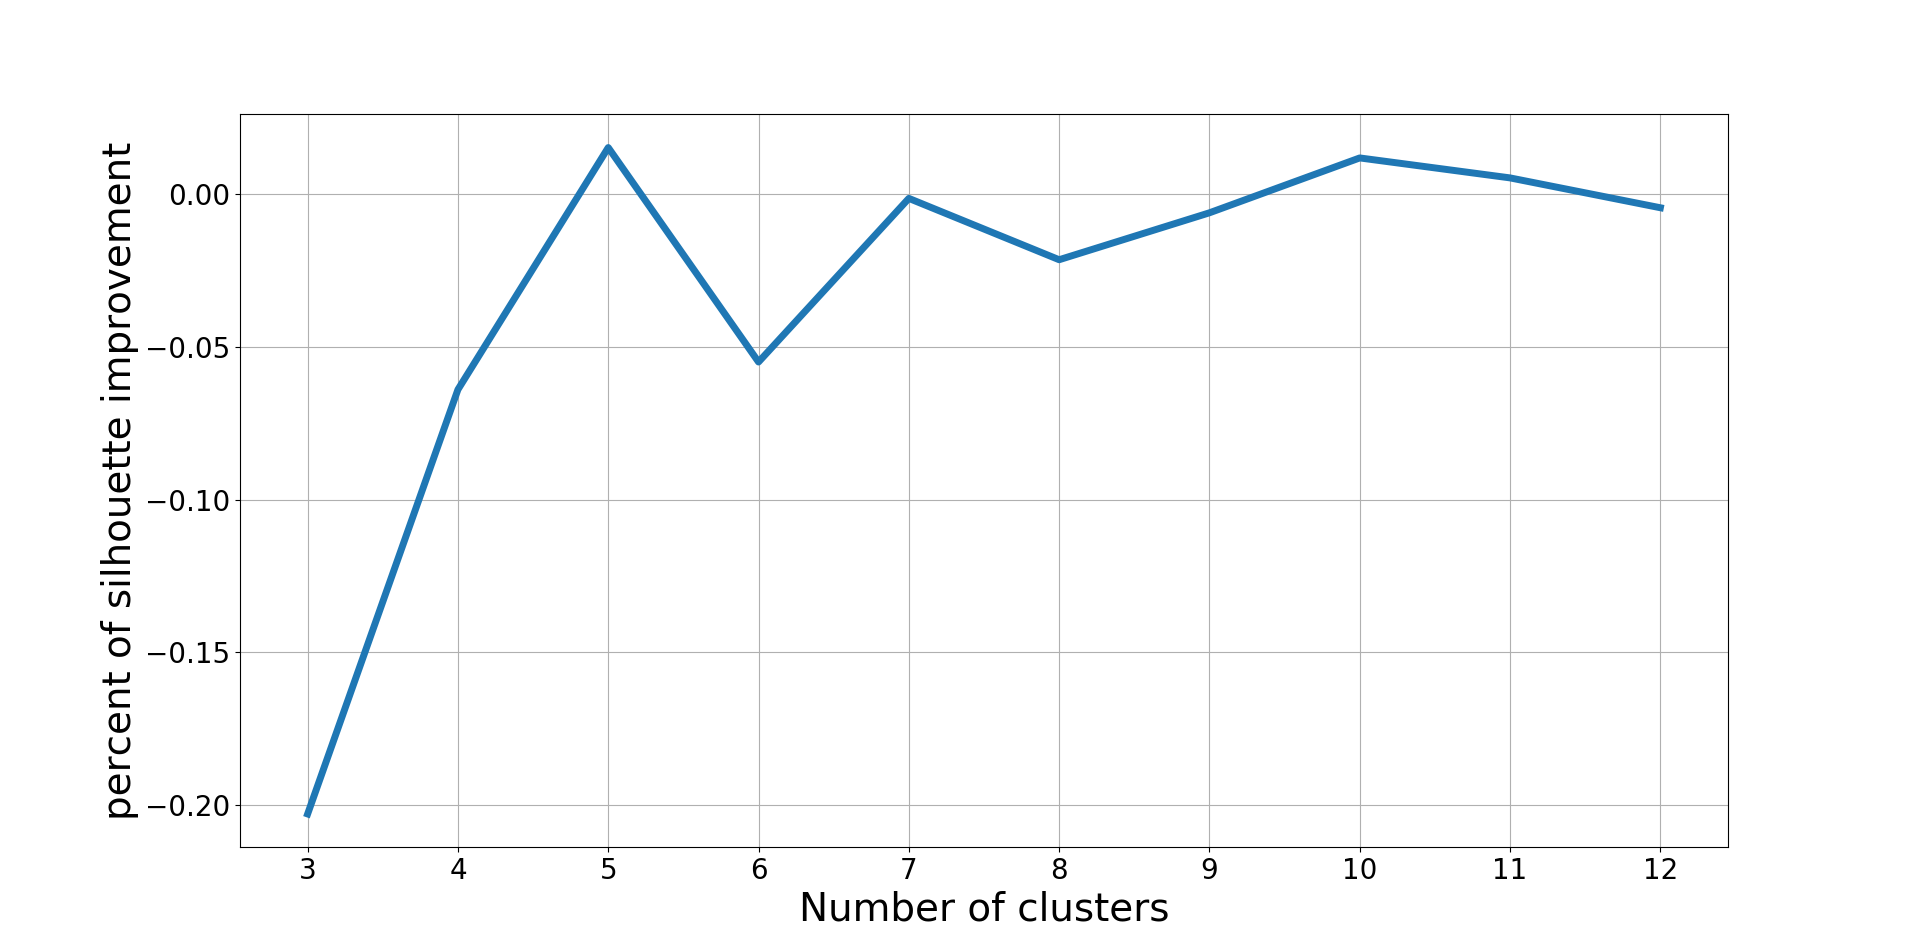
\includegraphics[scale=0.28]{num_of_clust_teams_shooting_pct_change.png}
\end{center}
\caption{Percentage of changes of silhouette scores}
\label{plt:clust_shooting_by_teams_plot2}
\end{figure}

The best value of silhouette score is for two clusters, but, as in the previous section, that number of clusters does not provide any interesting information and that is why we are looking at the improvement. The biggest positive improvement happened for five and ten clusters, but the one for five is higher.

\subsubsection{Results}
\label{subsubsec:clust_shooting_by_teams_results}

To conclude, there will be total of five clusters created by the K-Means.  Let's observe how many teams are there in the each cluster and from which seasons. Clusters can be seen in tables from \ref{tab:clust_shooting_by_teams_centr1} to \ref{tab:clust_shooting_by_teams_num5}.

\begin{table}[!h]
\begin{center}
\begin{tabular}{|c|c|c|c|c|} \hline
Area & Restricted area & Paint (non-ra) & Mid-range & Three pointer \\ \hline
Per game attempts & 31.4 & 12.6 & 20.2 & 19.6  \\ \hline
Totals attempts & 2541 & 1017 & 1634 & 1589  \\ \hline
Percentage & 37\% & 16\% & 24\% & 23\% \\ \hline
\end{tabular}
\caption{Centroid for cluster one}
\label{tab:clust_shooting_by_teams_centr1}
\end{center}
\end{table}

\begin{table}[!h]
\begin{tabular}{|c|c|c|c|c|c|c|c|c|c|} \hline
Season & 10-11 & 11-12 & 12-13 & 13-14 & 14-15 & 15-16 & 16-17 & 17-18 & 18-19 \\ \hline
\# of teams & 2 & 3 & 5 & 6 & 4 & 5 & 1 & 0 & 0 \\ \hline
\end{tabular}
\caption{Number of teams by season in cluster one}
\label{tab:clust_shooting_by_teams_num1}
\end{table}

Style from \textbf{cluster one} wasn't particulary popular during this decade because it represents teams that relied a lot on the inside scoring, where 37\% of their shots come from on average. 

\begin{table}[!h]
\begin{center}
\begin{tabular}{|c|c|c|c|c|} \hline
Area & Restricted area & Paint (non-ra) & Mid-range & Three pointer \\ \hline
Per game attempts & 25.6 & 12.7 & 26.4 & 17.0  \\ \hline
Totals attempts & 2070 & 1029 & 2141 & 1381  \\ \hline
Percentage & 31\% & 16\% & 32\% & 21\% \\ \hline
\end{tabular}
\caption{Centroid for cluster two}
\label{tab:clust_shooting_by_teams_centr2}
\end{center}
\end{table}

\begin{table}[!h]
\begin{tabular}{|c|c|c|c|c|c|c|c|c|c|} \hline
Season & 10-11 & 11-12 & 12-13 & 13-14 & 14-15 & 15-16 & 16-17 & 17-18 & 18-19 \\ \hline
\# of teams & 21 & 18 & 14 & 10 & 7 & 5 & 0 & 0 & 0 \\ \hline
\end{tabular}
\caption{Number of teams by season in cluster two}
\label{tab:clust_shooting_by_teams_num2}
\end{table}

\textbf{Cluster two }represents outdated shot selection, with a lot of mid-range shots. There are no teams today that are shooting just around 50\% of their shots as shots that produce more points per possession. This approach was very popular at the beginning of the decade, but died out with emergence of the Moreyball.

\begin{table}[!h]
\begin{center}
\begin{tabular}{|c|c|c|c|c|} \hline
Area & Restricted area & Paint (non-ra) & Mid-range & Three pointer \\ \hline
Per game attempts & 25.4 & 12.2 & 22.2 & 23.3  \\ \hline
Totals attempts & 2059 & 988 & 1800 & 1891  \\ \hline
Percentage & 31\% & 14\% & 27\% & 28\% \\ \hline
\end{tabular}
\caption{Centroid for cluster three}
\label{tab:clust_shooting_by_teams_centr3}
\end{center}
\end{table}

\begin{table}[!h]
\begin{tabular}{|c|c|c|c|c|c|c|c|c|c|} \hline
Season & 10-11 & 11-12 & 12-13 & 13-14 & 14-15 & 15-16 & 16-17 & 17-18 & 18-19 \\ \hline
\# of teams & 7 & 8 & 10 & 12 & 12 & 11 & 12 & 6 & 1 \\ \hline
\end{tabular}
\caption{Number of teams by season in cluster three}
\label{tab:clust_shooting_by_teams_num3}
\end{table}

Offense represented in \textbf{cluster three} was popular during more than half of the decade, peaking from 2012-13 to 2016-17 seasons. After that, there is a steep drop, with only one team from 2018-19, San Antonio Spurs. They were the 7th best offense in the league that year .

\begin{table}[!h]
\begin{center}
\begin{tabular}{|c|c|c|c|c|} \hline
Area & Restricted area & Paint (non-ra) & Mid-range & Three pointer \\ \hline
Per game attempts & 28.0 & 12.9 & 16.7 & 28.3  \\ \hline
Totals attempts & 2271 & 1042 & 1353 & 2290  \\ \hline
Percentage & 33\% & 15\% & 19\% & 33\% \\ \hline
\end{tabular}
\caption{Centroid for cluster four}
\label{tab:clust_shooting_by_teams_centr4}
\end{center}
\end{table}

\begin{table}[!h]
\begin{tabular}{|c|c|c|c|c|c|c|c|c|c|} \hline
Season & 10-11 & 11-12 & 12-13 & 13-14 & 14-15 & 15-16 & 16-17 & 17-18 & 18-19 \\ \hline
\# of teams & 0 & 1 & 0 & 1 & 6 & 8 & 14 & 20 & 14 \\ \hline
\end{tabular}
\caption{Number of teams by season in cluster four}
\label{tab:clust_shooting_by_teams_num4}
\end{table}

Teams in \textbf{cluster four} replaced mid-range shots with shots that produce more points per possession, which is a staple of modern offense. This shot selection became popular in 2016-17 and remains as such at the end of the decade.

\begin{table}[!h]
\begin{center}
\begin{tabular}{|c|c|c|c|c|} \hline
Area & Restricted area & Paint (non-ra) & Mid-range & Three pointer \\ \hline
Per game attempts & 30.1 & 12.9 & 10.5 & 33.9  \\ \hline
Totals attempts & 2437 & 1049 & 852 & 2742 \\ \hline
Percentage & 34\% & 15\% & 12\% & 39\% \\ \hline
\end{tabular}
\caption{Centroid for cluster five}
\label{tab:clust_shooting_by_teams_centr5}
\end{center}
\end{table}

\begin{table}[!h]
\begin{tabular}{|c|c|c|c|c|c|c|c|c|c|} \hline
Season & 10-11 & 11-12 & 12-13 & 13-14 & 14-15 & 15-16 & 16-17 & 17-18 & 18-19 \\ \hline
\# of teams & 0 & 0 & 1 & 1 & 1 & 1 & 3 & 4 & 15 \\ \hline
\end{tabular}
\caption{Number of teams by season in cluster five}
\label{tab:clust_shooting_by_teams_num5}
\end{table}

\textbf{Cluster five} is upgraded version of the cluster before it. Half of the league shot like this in 2018-19. Interesting thing is, this extreme approach wasn't that popular just a season prior, but it is possible that that was just a transition period during which teams started to eliminate mid-range shots. Teams from seasons before 2016-17 are all Houston Rockets, team that popularized Moreyball. 

\section{Classification}
\label{sec:cls}

Classification is a process of assigning categories to provided data points. It consists of two parts, training and testing. Classification model is created during the first part, while the second part is used to evaluate how good the created model is, with various methods.

During training, classification algorithm will be given some data points with assigned category. It's task is to, using those given data points, learn in which category to put every new data point with unknown category. There are a lot of different algorithms for classification, such as K-Nearest Neighbor (KNN), Support Vector Machines (SVM), Decision Trees and others. Which algorithm will be used depends on the data and situation. \cite{supervisedLearning}

Created model should not only do well on already seen, training data, but should also be able to correctly classify new, unseen, data. That, of course, might not always happen. That means that created model is either \textbf{underfit} or \textbf{overfit}. Underfitting means that model did not memorize patterns that appear in training data, and thus cannot classify it well. That also leads to bad results on test data. Overfitting means that model did memorize patterns in training data, but memorized them better than it should and is unable to generalize, so, in spite of having good results on train data, gives poor results on test data.

That can be avoided with \textbf{cross-validation}, validation techniques that can evaluate how well will model generalize new data. Evaluating can be done by dividing training data into two sets. First set will still be used in model creation, while the other, called validation set, is used for testing model during the \textit{training} phase in order to check how well will that model generalize and to limit overfitting and underfitting. Validation set and training set must be drawn from the same distribution! \cite{crossVal}

In order to create models, we split the data into two parts, train and test. It is important that those sets do not overlap! If they do, model cannot be trusted because we are testing it on data that model was trained on. Also, splitting must be random. If it isn't, there is a chance that model trains on data that belong only to one category, and that can lead to overfitting, because it will be unable to recognize other categories. \cite{crossVal}

Let's note that creating validation set will reduce number of samples in training data, which means that there is less data to train model on, which can lead to a model that did not memorize patterns well (underfitting). Method used to avoid that is called \textbf{K-Fold}, which can provide enough data for training and validating. In K-Fold, model will be created on train set, and then evaluated on validation set $K$ times, each time on different splits. Every data point gets to be in validation set once, and in the train set $K-1$ times. After evaluating each of the $K$ models, average will be computed. This method have shown best results when $K$ has a value of 3, 5 or 10. Special case of K-Fold is called Leave one Out, where $K$ equals number of data points in train set. This approach can be usefull if there is little data. Using random train/test split or K-Fold can lead to different distributions in different folds. To avoid that, method called stratification can be used. \cite{crossVal}

After training, model should be evaluated. For that, we are using test data because category for every data point from test is known to us, but not to a model, so we can observe how many categories are predicted correctly. Evaluation is done with various metrics. First we define the following:

\begin{itemize}
	\item \textbf{True positives (TP)}. Data points that are predicted to belong to category and actually belong to that category.
	\item \textbf{True negatives (TN)}. Data points that are predicted not to belong to category and actually do not belong to that category.
	\item \textbf{False positives (FP)}. Data points that are predicted to belong to category but actually do not belong to that category. 
	\item \textbf{False negatives (FN)}. Data points that are predicted not to belong to category, but actually belong to that category.
\end{itemize}

In other words, true data points are correctly predicted, so, good model is the one that maximizes number of TP and TN, while minimizing FP and FN. Now we can define some of the most used metrics. \textbf{Accuracy} is a ratio of correctly predicted data points to total number of data points. It is calculated as $(TP + TN) / (TP + TN + FP + FN)$. \textbf{Precision} is ratio of correctly predicted positive data points to the total predicted positive data points. Calculated as $TP / (TP + FP)$. \textbf{Recall} or Sensitivity is a ratio of correctly predicted positive data points from one category to the number of data points from that category. It is calculated as $TP / (TP + FN)$. \textbf{F1 score} is the weighted average of Precision and Recall. It takes into account both FP and FN. Calculated as $2 * (Precision * Recall) / (Precision + Recall)$.

These scores can have values from 0 to 1, with 1 being the perfect model, and 0 being model that can't classify anything correctly. Because those values are impossible to get, we want our model to have values for mentioned metrics as close to 1 as possible. Let's also note that accuracy is better to use on balanced datasets (each category has similar number of data points) while precision, recall and f1 score are better for unbalanced datasets.

The other thing we can do is compare results of trained model to random model (also called \textit{dummy}). That model will literally classify data points at random, so if our model has worse results than that (or similar), it is a bad model. 

Besides those, there are more ways to evaluate models, such as confusion matrices, log loss, ROC curves, cross-validation (can be used for testing also) etc.

\subsection{Classifying positions}
\label{subsec:pos_clf}

There are five traditional positions in basketball, PG, SG, SF, PF and C. Every position is asked to do different things during a game, for example, it is expected that centers have more rebounds per game than other positions because they are taller and are usually near basket. Guards are expected to shoot more 3-point shots, while point guards are expected to assist more, because the ball is mostly in their possession. Task is to classify position of a player based on his stats. Idea is to create model on the data from earlier seasons, and use it to classify players that play in the modern era. Errors are expected because positions are not as important, or not as well defined, as they were back in the day.

\subsubsection{Training model}
\label{subsubsec:pos_clf_training}

This is multiclass problem, because there are five positions (classes). Data used is per game data for seasons from 1985-86 to 2005-06. Stats used can be seen in table \ref{tab:pos_clf_data}. Data is also filtered and contains only players that played more than 15 minutes per game and more than 35 games in a single season. Filtering is done because the more time player spent on the floor, the more time he had to form his stats according to his playstyle. In total, there are 5417 players (1106 point guards, 1095 shooting guards, 1096 small forwards, 1120 power forwards and 1000 centers). Note that data is close to balanced.

\begin{table}[!h]
\begin{center}
\begin{tabular}{|c|c|} \hline
Non-shooting stats & Shooting stats \\ \hline
PTS & 3PA\\
AST & 3P\\
TRB & 2PA \\
ORB & 2P \\
DRB & FTA \\
AST & FT \\
BLK & \\
STL & \\
TOV & \\
PF & \\ \hline
\end{tabular}
\caption{Data for classification by position}
\label{tab:pos_clf_data}
\end{center}
\end{table}

First, let's compare stats by position. This will illustrate how hard it is to compare positions based only on selected traditional stats. Selected visualization method is box plot \cite{boxplots} because it shows distribution by stats and outliers. Some player might be better at something then most of other players at his position. Think of Westbrook and his rebounding, Jokić and passing or Brook Lopez and Karl-Anthony Towns and three point shooting. Those players are outliers in those areas, and should be considered when building a model. Overall, some patterns definitely exists. Figures \ref{plt:pos_clf_data_boxplt1} and \ref{plt:pos_clf_data_boxplt2} are showing some of the stats by position.

\begin{figure}[h!]
\begin{center}
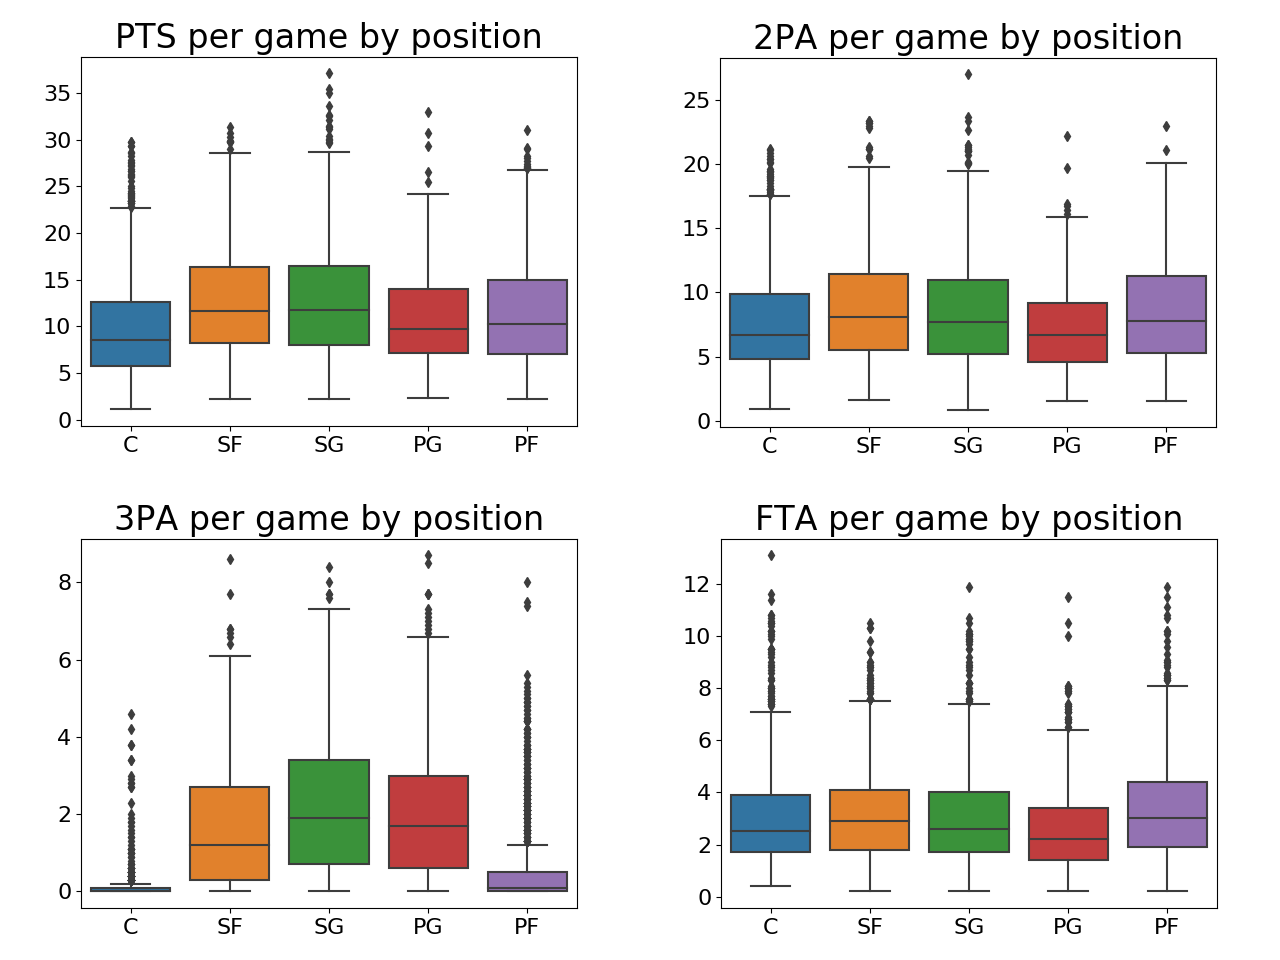
\includegraphics[width=1\textwidth]{per_pos_pts_shooting.png}
\end{center}
\caption{Shooting and points per game stats per position}
\label{plt:pos_clf_data_boxplt1}
\end{figure}

The only stat that is noticeably different for different positions in the first figure is 3PA per game. What we see is expected, because tall players are worse at 3-point shooting than guards and wings. Note that centers rarely shot any three-pointers back in the day (data is from 1985-85 to 2005-06), but there were some who shot more than the average shooting guard for example. Other stats have similar distributions for every positions, and might influence our classification less than three-point shooting.

\begin{figure}[h!]
\begin{center}
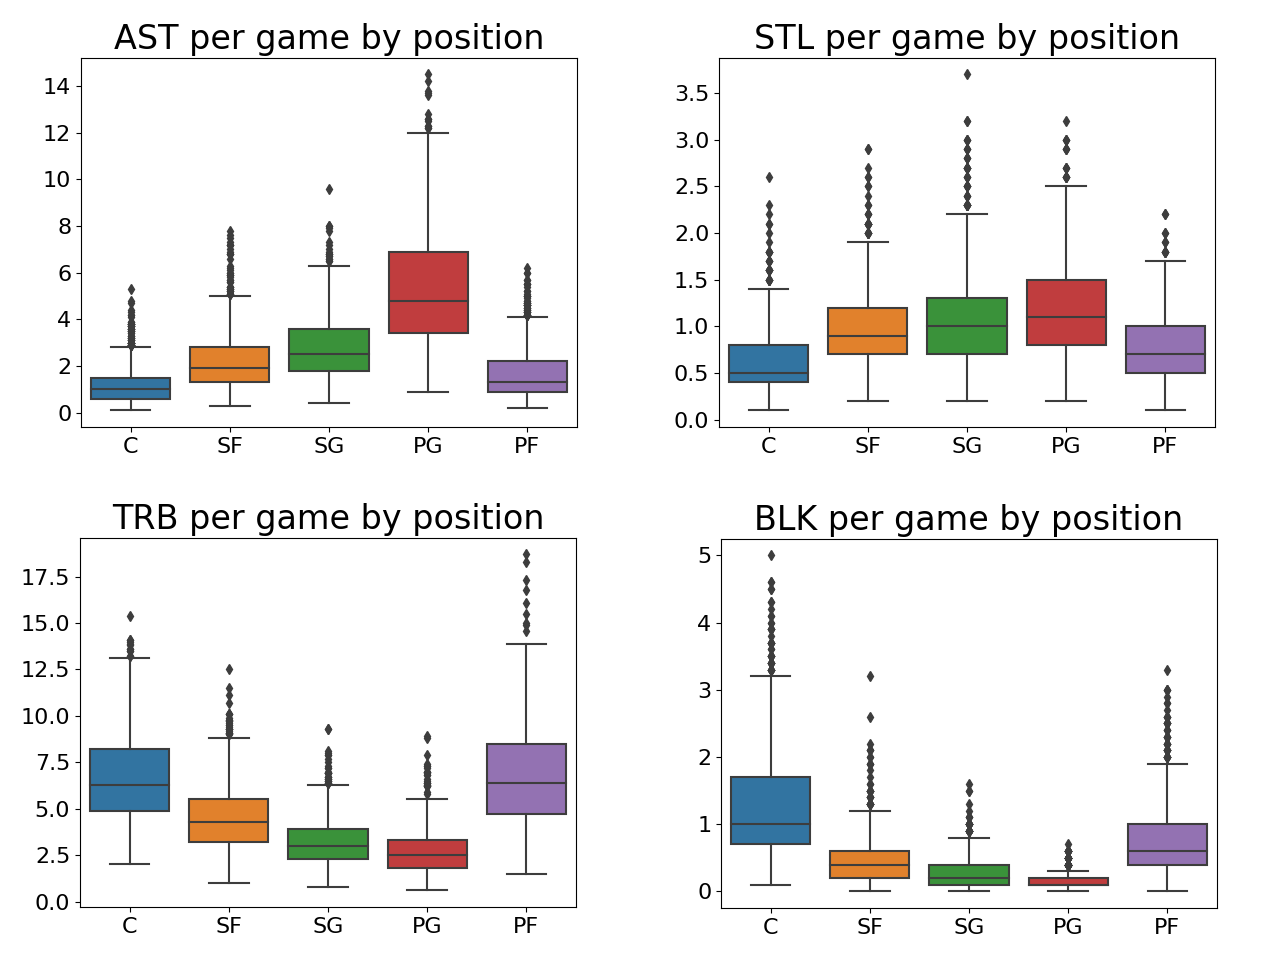
\includegraphics[width=1\textwidth]{per_pos_ast_stl_trb_blk.png}
\end{center}
\caption{Various stats per position}
\label{plt:pos_clf_data_boxplt2}
\end{figure}

In the second figure difference by position can be easily noticed for selected stats. Point guards had the most assists per game by far. They are also first in steals per game, but last in blocks and rebounds per game. Opposite applies to the centers and power forwards. To conclude, player that had a lot of assists and three-pointers per game were probably PGs and a good rebounder and blocker is probably center.

After these examinations, we can start with training! Data is divided into two sets, train (70\% of the data) and test (30\% of the data). Models are trained with method called \textit{Grid search}. Grid search takes into account every combination of provided parameters we want to test, and returns model created with combination that has highest value for selected metric. In this case, selected metric is accuracy because data is fairly balanced. Models are trained with stratified K-Fold ($K = 5$) \cite{crossVal} cross-validation method, in order to avoid overfitting and underfitting.

In total, four classifiers are used: K-Nearest Neighbor Classifier (\textbf{KNN}), Random Forests Classifier (\textbf{RFC}), Gradient Boosting Classifier (\textbf{GBC}) and Support Vector Classifier (\textbf{SVC}).

\subsubsection{Evaluation}
\label{subsubsec:pos_clf_eval}

Here we will examine how models perform on unknown data. Basic metrics such as accuracy, precision, recall and f1 score for every model are shown in the table \ref{tab:pos_clf_models}).

\begin{table}[!h]
\begin{center}
\begin{tabular}{|c|c|c|c|c|} \hline
Model & Accuracy & Precision & Recall & F1 score \\ \hline
KNN & 0.63 & 0.63 & 0.63 & 0.63 \\ \hline
RFC & 0.69 & 0.69 & 0.69 & 0.69 \\ \hline
GBC & 0.70 & 0.71 & 0.71 & 0.71 \\ \hline
SVC & 0.70 & 0.71 & 0.70 & 0.70 \\ \hline
\end{tabular}
\caption{Model evaluation}
\label{tab:pos_clf_models}
\end{center}
\end{table}

RFC, GBC and SVC are better than KNN and have similar results. Accuracy is fairly high and is definitely influenced by different playstyles of players on the same positions. Other metrics have similar or same values as accuracy. Note that it is possible to check how good are the models at classifying each of the positions separately (Tables \ref{tab:pos_clf_knn}, \ref{tab:pos_clf_rfc}, \ref{tab:pos_clf_gbc} and \ref{tab:pos_clf_svc}). 
Position that is the easiest to predict correctly is point guard, while forward positions (PF and SF) are the hardest.

\begin{table}[!h]
\begin{center}
\begin{tabular}{|c|c|c|c|} \hline
Position \textbackslash Metric & Precision & Recall & F1 score \\ \hline
PG & 0.86 & 0.85 & 0.85 \\ \hline
SG & 0.60 & 0.62 & 0.61 \\ \hline
SF & 0.56 & 0.51 & 0.54 \\ \hline
PF & 0.53 & 0.57 & 0.55 \\ \hline
C & 0.62 & 0.61 & 0.62 \\ \hline
\end{tabular}
\caption{KNN metrics by class}
\label{tab:pos_clf_knn}
\end{center}
\end{table}

\begin{table}[!h]
\begin{center}
\begin{tabular}{|c|c|c|c|} \hline
Position \textbackslash Metric & Precision & Recall & F1 score \\ \hline
PG & 0.89 & 0.86 & 0.87 \\ \hline
SG & 0.66 & 0.72 & 0.69 \\ \hline
SF & 0.63 & 0.58 & 0.60 \\ \hline
PF & 0.60 & 0.63 & 0.62 \\ \hline
C & 0.69 & 0.67 & 0.68 \\ \hline
\end{tabular}
\caption{RFC by class}
\label{tab:pos_clf_rfc}
\end{center}
\end{table}

\begin{table}[!h]
\begin{center}
\begin{tabular}{|c|c|c|c|} \hline
Position \textbackslash Metric & Precision & Recall & F1 score \\ \hline
PG & 0.89 & 0.87 & 0.88 \\ \hline
SG & 0.69 & 0.70 & 0.70 \\ \hline
SF & 0.65 & 0.61 & 0.63 \\ \hline
PF & 0.61 & 0.65 & 0.62 \\ \hline
C & 0.69 & 0.69 & 0.69 \\ \hline
\end{tabular}
\caption{GBC by class}
\label{tab:pos_clf_gbc}
\end{center}
\end{table}

\begin{table}[!h]
\begin{center}
\begin{tabular}{|c|c|c|c|} \hline
Position \textbackslash Metric & Precision & Recall & F1 score \\ \hline
PG & 0.89 & 0.87 & 0.88 \\ \hline
SG & 0.69 & 0.70 & 0.70 \\ \hline
SF & 0.65 & 0.61 & 0.63 \\ \hline
PF & 0.61 & 0.65 & 0.62 \\ \hline
C & 0.69 & 0.69 & 0.69 \\ \hline
\end{tabular}
\caption{SVC by class}
\label{tab:pos_clf_svc}
\end{center}
\end{table}

We also have to check if the models are better than random (dummy) classifier (table \ref{tab:pos_clf_dummy}). Dummy classifier will classify data based on training set class distribution. Classes are close to balanced, and there are five of them, so accuracy is expected to be around 0.20.

\begin{table}[!h]
\begin{center}
\begin{tabular}{|c|c|c|c|c|} \hline
Model & Accuracy & Precision & Recall & F1 score \\ \hline
Dummy & 0.19 & 0.19 & 0.19 & 0.19 \\ \hline
\end{tabular}
\caption{Model evaluation}
\label{tab:pos_clf_dummy}
\end{center}
\end{table}

Every trained model is better than the random model in every metric by a significant margin.

Important step is to cross-validate models, to check whether or not they overfit. Cross-validation can be influenced by distribution of the classes in the train and test sets which should be close to equal for every class. In this case, as we can see from table \ref{tab:pos_clf_cross_val}, distribution is similar.

\begin{table}[!h]
\begin{center}
\begin{tabular}{|c|c|c|c|c|c|} \hline
Set & PG \% & SG \% & SF \% & PF \% & C \% \\ \hline
Train & 21\% & 21\% & 20\% & 20\%  & 18\% \\ \hline
Test & 19\% & 19\% & 22\% & 22\% & 18\% \\ \hline
\end{tabular}
\caption{Model evaluation}
\label{tab:pos_clf_cross_val}
\end{center}
\end{table}

Cross-validation accuracy for $K = 5$ and 95\% confidence intervals are shown in table \ref{tab:pos_clf_cross_val_eval}. Every model has cross-validated accuracy score that is close to it's real accuracy score.

\begin{table}[!h]
\begin{center}
\begin{tabular}{|c|c|c|} \hline
Model & Cross-validation accuracy & 95\% confidence interval \\ \hline
KNN & 0.61 & +/- 0.05 \\ \hline
RFC & 0.68 & +/- 0.05 \\ \hline
GBC & 0.68 & +/- 0.07 \\ \hline
SVC & 0.68 & +/- 0.06 \\ \hline
\end{tabular}
\caption{Cross-validation}
\label{tab:pos_clf_cross_val_eval}
\end{center}
\end{table}

\subsubsection{Results}
\label{subsubsec:pos_clf_res}

With training and testing finished we can now give our models some data, and observe results. Let's see how well models classify some of the active players \textbf{from 2018-19 season} who were divided in groups, not by position, but by their playstyle. Tables \ref{tab:pos_clf_c_pf_predictions} (for C and PF) and \ref{tab:pos_clf_pg_sg_sf_predictions} (for PG, SG and SF) contain predictions for every model for some of the players along with their actual, listed position.

\begin{table}[!h]
\begin{center}
\begin{tabular}{|c|c|c|c|c|c|} \hline
\multicolumn{6}{|c|}{\textbf{Passing bigs}} \\ \hline
\textbf{Player} & \textbf{Listed} & \textbf{KNN} & \textbf{RFC} & \textbf{GBC} & \textbf{SVC} \\ \hline
Nikola Jokić & C & PF & PF & PF & PF \\ \hline
Draymond Green & PF & PG & SF & PF & SF \\ \hline
\multicolumn{6}{|c|}{\textbf{Shooting bigs}} \\ \hline
\textbf{Player} & \textbf{Listed} & \textbf{KNN} & \textbf{RFC} & \textbf{GBC} & \textbf{SVC} \\ \hline
Brook Lopez & C & SF & PF  & PF & PF \\ \hline
Karl-Anthony Towns & C & PF  & PF & PF & PF  \\ \hline
\multicolumn{6}{|c|}{\textbf{Rim runners}} \\ \hline
\textbf{Player} & \textbf{Listed} & \textbf{KNN} & \textbf{RFC} & \textbf{GBC} & \textbf{SVC} \\ \hline
Jarrett Allen & C & PF & C & C & C  \\ \hline
Clint Capela & C & C & C & C & C \\ \hline
\multicolumn{6}{|c|}{\textbf{Stretch fours}} \\ \hline
\textbf{Player} & \textbf{Listed} & \textbf{KNN} & \textbf{RFC} & \textbf{GBC} & \textbf{SVC} \\ \hline
Dāvis Bertāns & PF & SF & PF & SF & PF \\ \hline
Kevin Love & PF & PF & PF & PF & PF \\ \hline
\multicolumn{6}{|c|}{\textbf{Various}} \\ \hline
\textbf{Player} & \textbf{Listed} & \textbf{KNN} & \textbf{RFC} & \textbf{GBC} & \textbf{SVC} \\ \hline
Hassan Whiteside & C & C & C & C & C \\ \hline
Andre Drummond & C & PF & PF & PF & PF \\ \hline
Giannis Antetokounmpo & PF & PF & PF & PF & PF \\ \hline
Anthony Davis & C & PF & PF & PF & PF \\ \hline
Blake Griffin & PF & SG & PF & SG & SF \\ \hline
\end{tabular}
\caption{Predictions for centers and power forwards}
\label{tab:pos_clf_c_pf_predictions}
\end{center}
\end{table}

\begin{table}[!h]
\begin{center}
\begin{tabular}{|c|c|c|c|c|c|} \hline
\multicolumn{6}{|c|}{\textbf{Three and D players}} \\ \hline
\textbf{Player} & \textbf{Listed} & \textbf{KNN} & \textbf{RFC} & \textbf{GBC} & \textbf{SVC} \\ \hline
Danny Green & SG & SF & PF & PF & SF \\ \hline
Klay Thompson & SG & SF & SG & SF & SG  \\ \hline
Eric Gordon & SG & SG & SG & SG & SG  \\ \hline
Jae Crowder & SF & SF & SF & SF & SF  \\ \hline
\multicolumn{6}{|c|}{\textbf{Pass first guards}} \\ \hline
\textbf{Player} & \textbf{Listed} & \textbf{KNN} & \textbf{RFC} & \textbf{GBC} & \textbf{SVC} \\ \hline
Ricky Rubio & PG & PG & PG & PG & PG \\ \hline
Elfrid Payton & PG & PG & PG & PG & PG \\ \hline
\multicolumn{6}{|c|}{\textbf{Scoring guards}} \\ \hline
\textbf{Player} & \textbf{Listed} & \textbf{KNN} & \textbf{RFC} & \textbf{GBC} & \textbf{SVC} \\ \hline
Stephen Curry & PG & SG & SG & SG & PG  \\ \hline
James Harden & PG & SG & SG & SG & PG \\ \hline
Damian Lillard & PG & SG & PG & PG & PG \\ \hline
\multicolumn{6}{|c|}{\textbf{Various}} \\ \hline
\textbf{Player} & \textbf{Listed} & \textbf{KNN} & \textbf{RFC} & \textbf{GBC} & \textbf{SVC} \\ \hline
LeBron James & SF & SF & SF & SF & SF \\ \hline
Russell Westbrook & PG & PF & SF & PG & PG \\ \hline
Ben Simmons & PG & PF & PF & PF & SF \\ \hline
Hassan Whiteside & C & C & C & C & C \\ \hline
Andre Drummond & C & PF & PF & PF & PF \\ \hline
Anthony Davis & C & PF & PF & PF & PF \\ \hline
Harrison Barnes & PF-SF & SF & SF & SF & SF \\ \hline
Buddy Hield & SG & SF & SF & SF & SF \\ \hline
Blake Griffin & PF & SG & PF & SG & SF \\ \hline
\end{tabular}
\caption{Predictions for guards and small forwards}
\label{tab:pos_clf_pg_sg_sf_predictions}
\end{center}
\end{table}

Players that played similar to their traditional position counterpart (e.g. passing guards and rim runners) are classified mostly correctly. Others mostly weren't. This means that this era of basketball has a lot of untraditional players, which is expected because nowadays, players are asked to do a lot of different things. Interestingly, the best rebounder in the NBA today, Andre Drummond is classified as a PF, and some classifiers predicted that Draymond Green is a PG and that Danny Green is a PF. 

\subsubsection{Conclusion}
\label{subsubsec:pos_clf_conclusion}

Models created are fairly accurate. Data used for training spans multiple eras of basketball and that probably had influence on models' performance because playstyles were different. Also, players on the same positions during same era can be specialized in different things. Despite that, classifying algorithms managed to recognize some patterns in the data and because of that models are not bad. Classifying players from 2018-19 on models created on data from 1985-86 to 2005-06 had interesting results. 

\subsection{Will rookie be an All-Star during his career?}
\label{subsec:rookie_to_all_star}

In this section, we will analyze whether or not a player will be named an All-Star during his career based just on stats from his rookie season. This method is not fair, because players shouldn't be judged on their rookie season performance. For example, Giannis Antetokounmpo, NBA MVP for the 2018-19 season, had a rather underwhelming rookie season. Also, there are players that, it appears, peaked during their first season, such as Tyreke Evans or Michael Carter-Williams. So, it is possible for a player that was not good during his rookie season to drastically improve and become an All-Star and/or All-NBA type of player at some point of his career. It is not just possible for a player to improve, it is also expected from him to, as he gain more experience.

\subsubsection{Data}
\label{subsubsec:data_all_star}

Data used is from \href{https://www.basketball-reference.com/}{Basketball-reference.com} and includes stats from rookie seasons of every lottery pick (first 14 selections) from 2000 NBA draft to 2016 NBA draft. It includes total of 237 seasons. Note that only lottery pick drafted during that span that did not play in the NBA is Fran Vazquez. Stats taken into consideration for model creation are:

\begin{itemize}
	\item \textbf{PTS}, Points per game
	\item \textbf{TRB}, Rebounds per game
	\item \textbf{AST}, Assists per game
	\item \textbf{STL}, Steals per game
	\item \textbf{BLK}, Blocks per game
	\item \textbf{TS\%}, True shooting percentage
	\item \textbf{3PAr}, Three-point attempt rate
	\item \textbf{FTr}, Free throw attempt rate
	\item \textbf{WS}, Win shares
	\item \textbf{OBPM}, Offensive box plus/minus
	\item \textbf{DBPM}, Defensive box plus/minus
	\item \textbf{VORP}, Value over replacement player
	\item \textbf{Draft Pick}, draft position player is selected on
\end{itemize}

The first five are just regular traditional stats, something that most of the people would look at first. Next three are there because shooting should be taken into consideration. Offensive and defensive box plus/minus are advanced stats that are evaluating offense and defense of a player using box score of a player. Besides them, there are two more advanced stats that are good at evaluating player's performance. Draft pick is there because it is important where a player is selected.

\subsubsection{Plots}
\label{subsubsec:plots_all_stars}

Before we start with modeling, we should check is there any difference between rookie seasons of the players that will be All-Stars and players that won't. First, lets see the difference in draft position, points per game and Offensive and defensive box plus/minus stats. Those stats are shown with box plot \cite{boxplots} and can be seen in figure \ref{plt:box_plots_all_star}.

\begin{figure}[h!]
\begin{center}
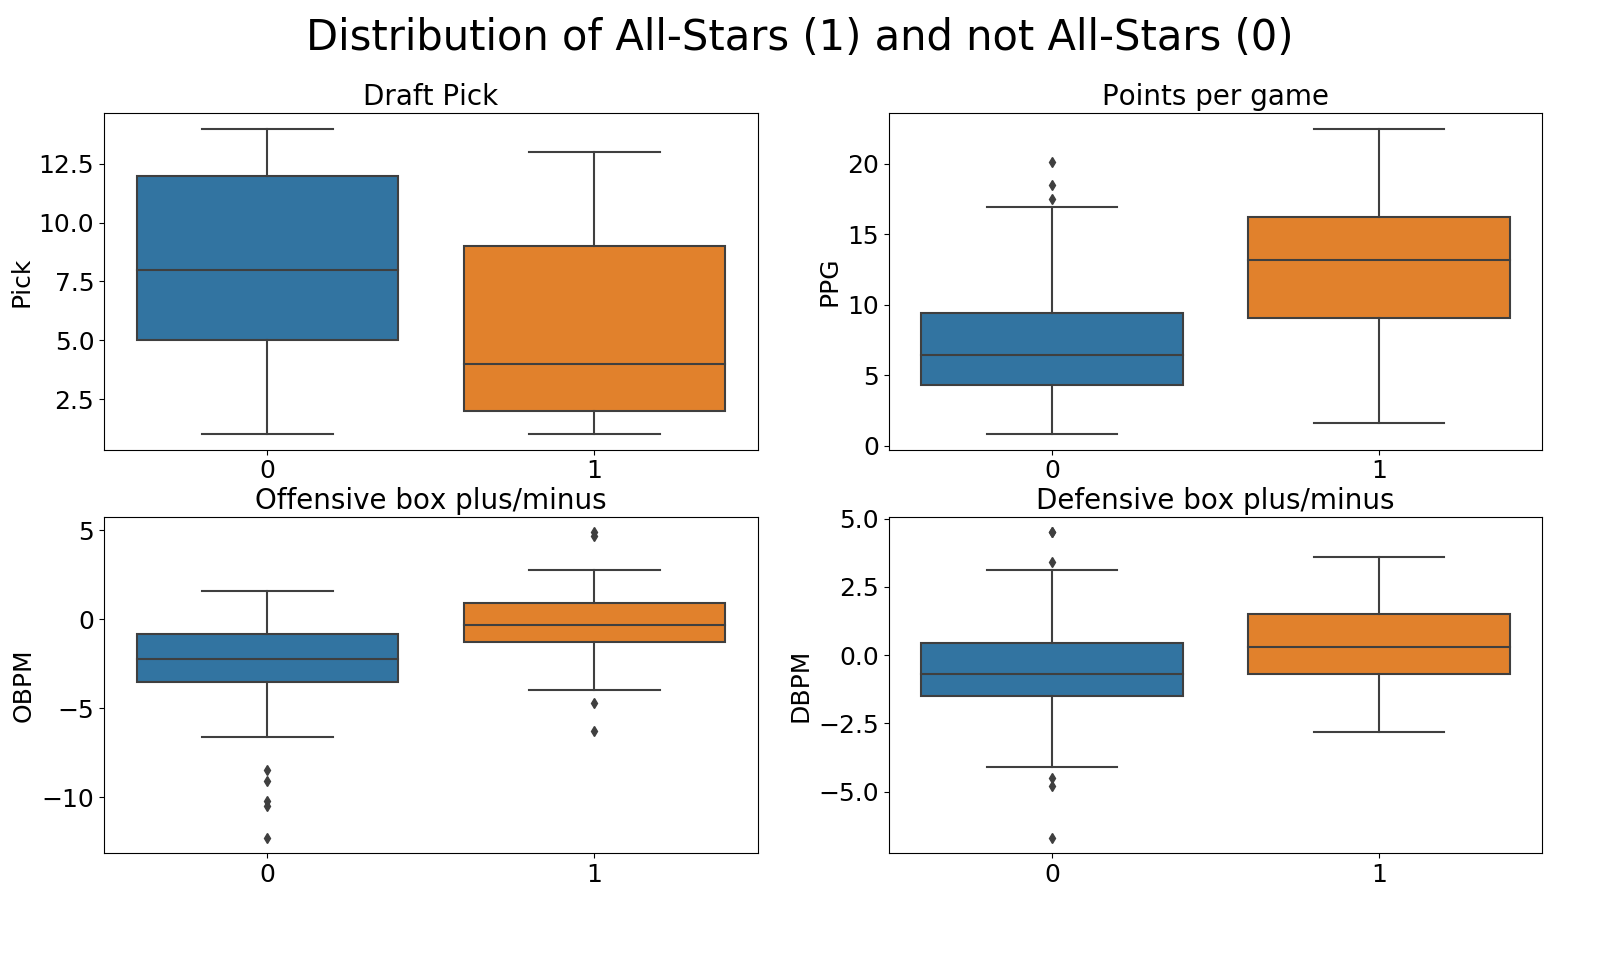
\includegraphics[scale=0.3]{box_plots_all_star.png}
\end{center}
\caption{Box plots for different stats}
\label{plt:box_plots_all_star}
\end{figure}

From the previous figure, we can see that future All-Stars are usually selected before players that won't become one. Difference in points per game is easily noticeable. As far as box plus/minus stats go, values for future All-Stars are slightly higher. Let's also take a look at the distribution plots for rebounds per game and assists per game (figure \ref{plt:trb_ast_all_star}) and for win shares \ref{plt:ws_all_star}.

\begin{figure}[h!]
\begin{center}
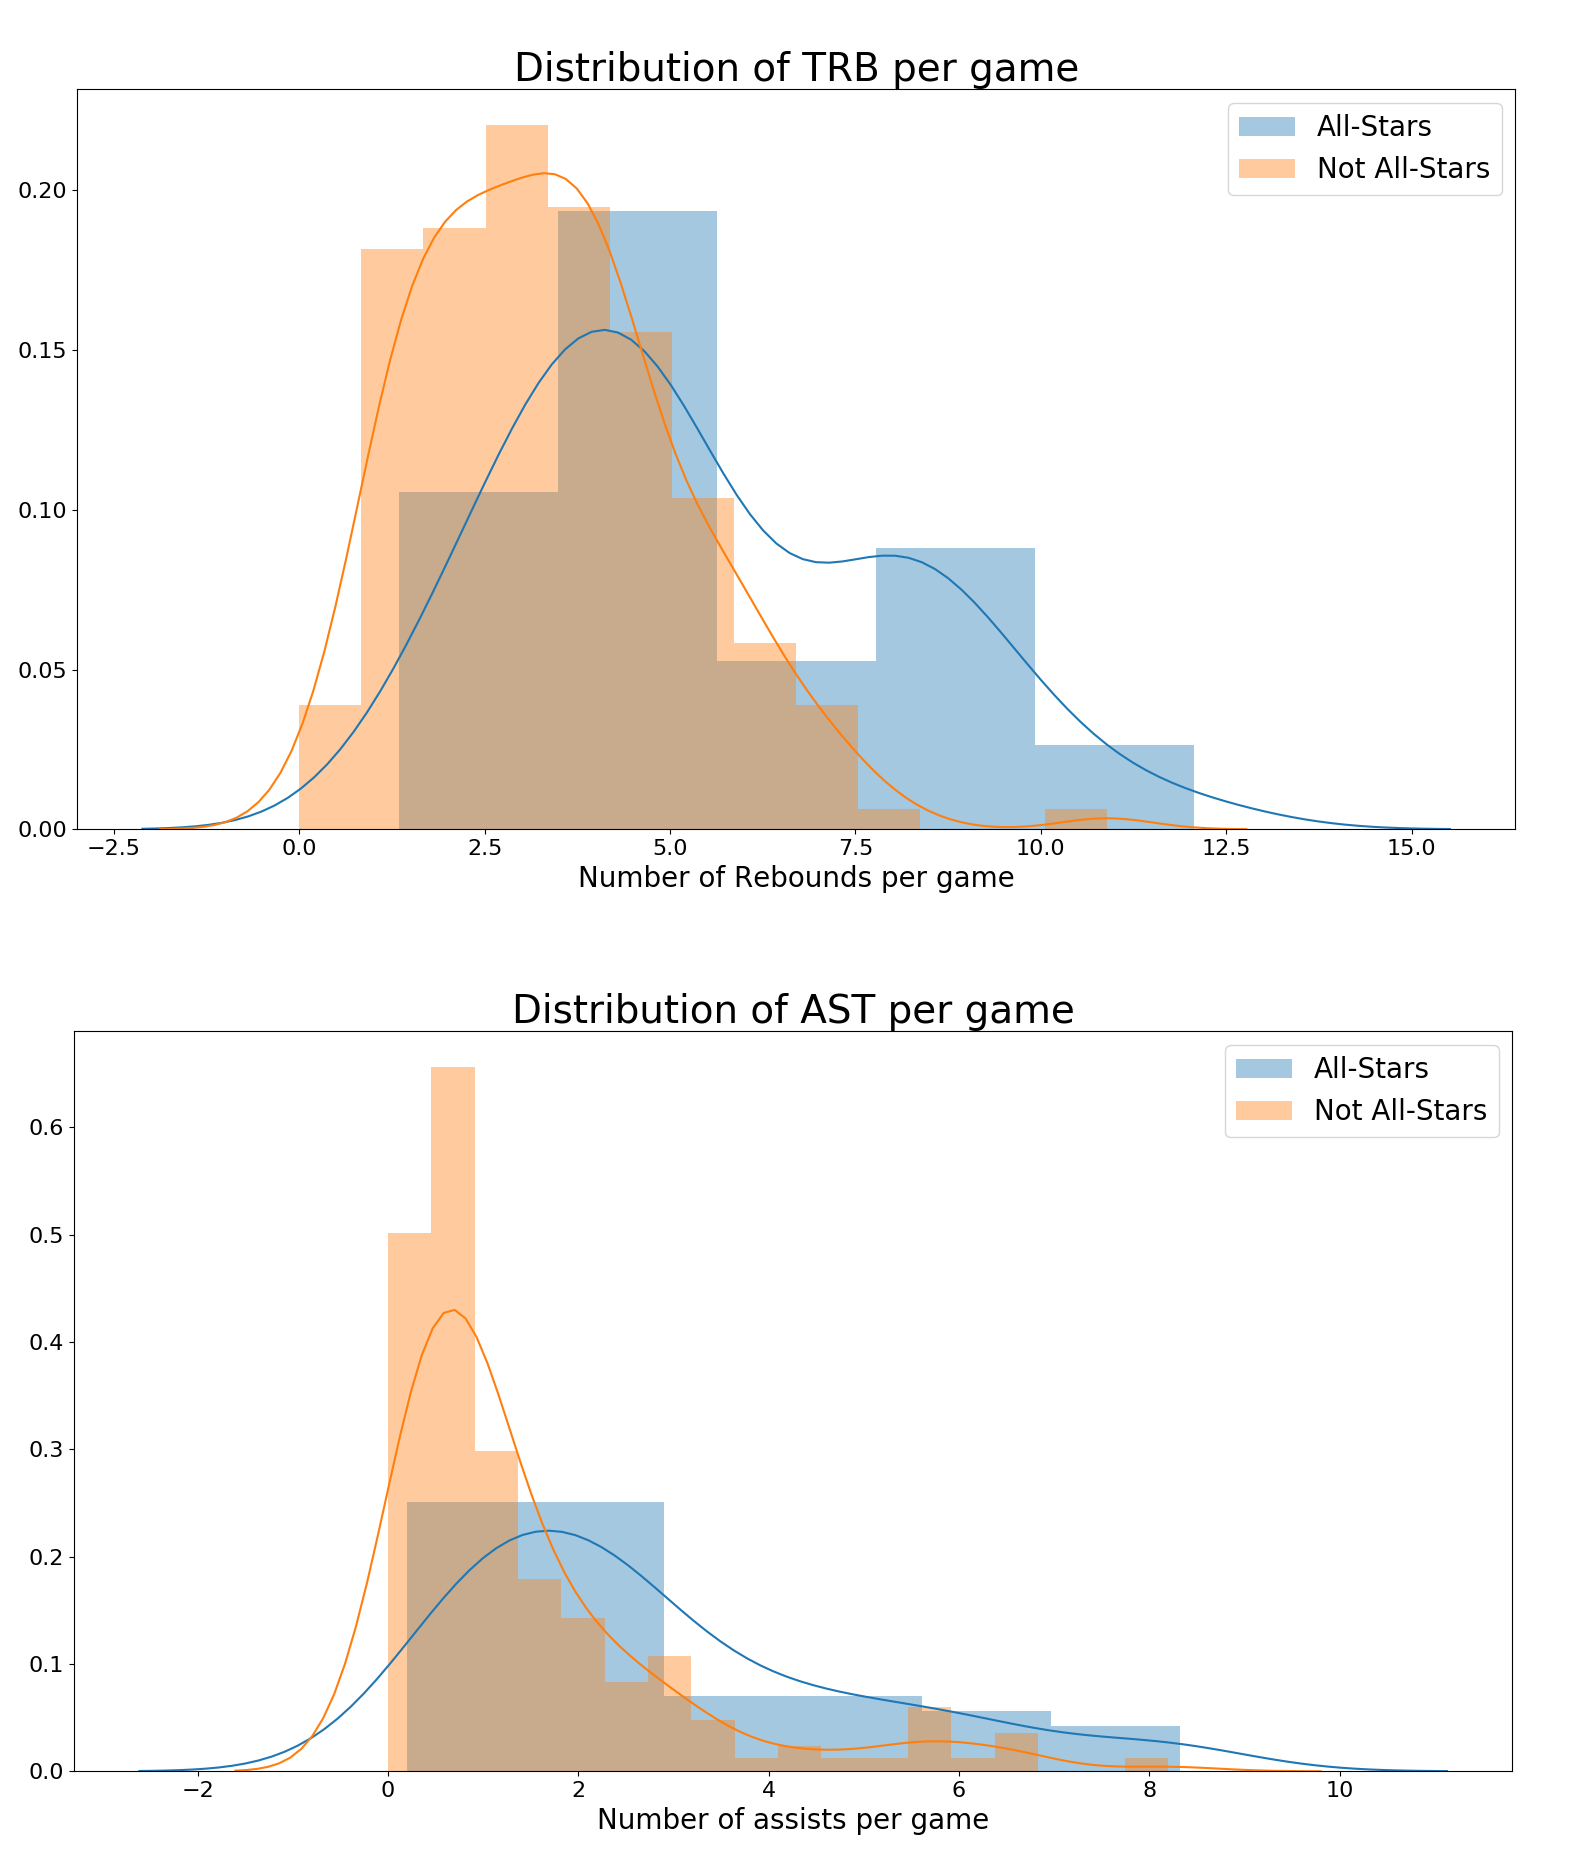
\includegraphics[scale=0.38]{trb_ast_all_star.png}
\end{center}
\caption{Distribution of AST and TRB per game}
\label{plt:trb_ast_all_star}
\end{figure}

\begin{figure}[h!]
\begin{center}
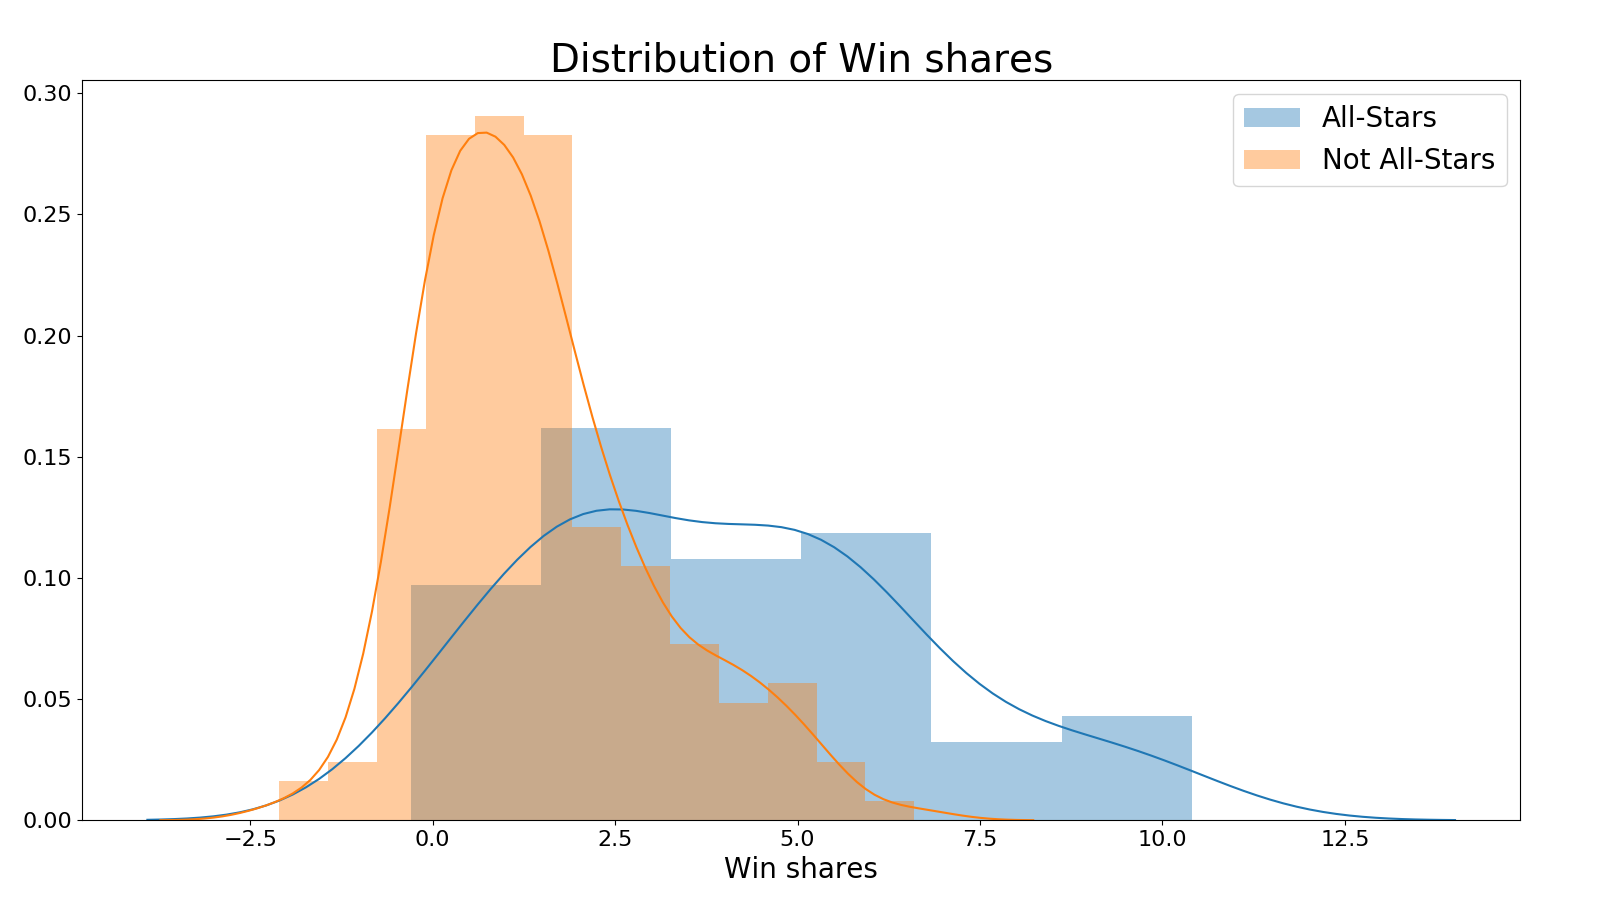
\includegraphics[scale=0.31]{ws_all_star.png}
\end{center}
\caption{Distribution of WS}
\label{plt:ws_all_star}
\end{figure}

We can notice the same pattern for these stats, the future All-Stars do have more rebounds per game, assists per game and win shares in their rookie seasons when compared to the other players. This tells us that there are patterns models can use to classify future All-Stars.

\subsubsection{Model creation}
\label{subsubsec:model_creation_all_star}

Out of 237 rookie seasons in the data 52 are from the future All-Stars (roughly 22\%). Before model creation we are splitting the data into two sets, train (70\% of the data) and test (30\% of the data). There are three different type of models that will be created, Random Forest Classifier (\textbf{RFC}), Support Vector Classifier (\textbf{SVC}) and Gradient Boosting Classifier (\textbf{GBC}).

This classification is binary classification, where result can be only two different classes, All-Star and not All-Star. For us, it is important to correctly classify players that will become All-Stars. Because of that, we want models that have high recall!

Parameters for models are selected with method called Grid Search that takes into account every combination of provided parameters we would like to test, and returns a model that is the 'best' for provided metric. In this case those metrics will be accuracy and recall. There will be six models in total, one RFC with the best accuracy and one with the best recall, one SVC with the best accuracy and one with the best recall and in the end one GBC with the best accuracy and one with the best recall. In order to minimize overfitting and underfitting, cross-validation method called stratified K-Fold \cite{crossVal} is used, where value of $K$ equals five.

\subsubsection{Model evaluation}
\label{subsubsec:model_eval_all_star}

Now, let's see how well created models preform on the test data (table \ref{tab:models_all_star}).

\begin{table}[!h]
\begin{center}
\begin{tabular}{|c|c|c|c|c|} \hline
\multicolumn{5}{|c|}{\textbf{Models with the best accuracy}} \\ \hline
\textbf{Model} & \textbf{Accuracy} & \textbf{Precision} & \textbf{Recall} & \textbf{F1 score} \\ \hline
SVC & \textbf{0.82} & 0.75 & 0.66 & 0.69 \\ \hline
RFC & \textbf{0.85} & 0.80 & 0.72 & 0.75 \\ \hline
GBC & \textbf{0.83} & 0.78 & 0.69 & 0.72 \\ \hline
\multicolumn{5}{|c|}{\textbf{Models with the best recall}} \\ \hline
\textbf{Model} & \textbf{Accuracy} & \textbf{Precision} & \textbf{Recall} & \textbf{F1 score} \\ \hline
SVC & 0.79 & 0.69 & \textbf{0.64} & 0.66 \\ \hline
RFC & 0.82 & 0.75 & \textbf{0.66} & 0.69 \\ \hline
GBC & 0.79 & 0.69 & \textbf{0.67} & 0.68 \\ \hline
\end{tabular}
\caption{Models created for All-Star classification}
\label{tab:models_all_star}
\end{center}
\end{table}

Created models does have high values for some of the metrics. Also, models have similar results. The worst value for accuracy, out of every models with the best accuracy, is SVC. Same can be also said about SVC in recall group, though values are not different much. These models are looking okay in a vacuum, but additional test have to done for us to be sure about that. First, we will check are these models better than the model that classifies rookie seasons at random (table \ref{tab:dummy_all_star}).

\begin{table}[!h]
\begin{center}
\begin{tabular}{|c|c|c|c|c|} \hline
\textbf{Model} & \textbf{Accuracy} & \textbf{Precision} & \textbf{Recall} & \textbf{F1 score} \\ \hline
Random & 0.56 & 0.44 & 0.42 & 0.43 \\ \hline
\end{tabular}
\caption{Random (dummy) classifier}
\label{tab:dummy_all_star}
\end{center}
\end{table}

We can see that our models are indeed better than the random one, with higher values for  every metric, which is good. After this, we want to check models for overfitting. First thing we would like to check is distribution of All-Stars in both train and test sets, which should be similar. Distributions are almost the same, train set has 22\% of the All-Stars while test set has 21\%. We will continue this by cross-validating (CV) models. Results are shown in the table \ref{tab:cross_val_all_star}. The results are close to to the actual score for the models with best accuracy, which is fine. Same cannot be said for models with best recall, because they might overfitt, which is not good.

\begin{table}[!h]
\begin{center}
\begin{tabular}{|c|c|c|} \hline
\multicolumn{3}{|c|}{\textbf{Models with the best accuracy}} \\ \hline
\textbf{Model} & \textbf{CV score (for accuracy)} & \textbf{95\% confidence interval} \\ \hline
SVC & 0.83 & +/- 0.07 \\ \hline
RFC & 0.83 & +/- 0.14 \\ \hline
GBC & 0.82 & +/- 0.11 \\ \hline
\multicolumn{3}{|c|}{\textbf{Models with the best recall}} \\ \hline
\textbf{Model} & \textbf{CV score (for recall)} & \textbf{95\% confidence interval} \\ \hline
SVC & 0.30 & +/- 0.33 \\ \hline
RFC & 0.48 & +/- 0.37 \\ \hline
GBC & 0.50 & +/- 0.30 \\ \hline
\end{tabular}
\caption{Cross-validation score}
\label{tab:cross_val_all_star}
\end{center}
\end{table}

In the end, we would like to test models for two more metrics, Log loss and AUC-ROC curve. We would like our loss to be as low as possible, so models that have Log loss close to \textbf{zero} are good. \cite{logLoss} 

If AUC (area under the ROC curve) is \textbf{one} that means our models can classify data perfectly (every data point that should be class A will belong to class A). If it is close to, or \textbf{0.5}, model cannot distinguish between classes and models where AUC is close to \textbf{zero} are reciprocating classes (every data point that should be class A will be class B and vice versa). That means that values further from 0.5 and closer to one are good \cite{aucRoc}.

As seen in table \ref{tab:aucroc_logloss_all_star} created models are mostly good. Gradient boosting appears to be poorer than we originally thought for both the best accuracy and recall. Note that Random forest models had the best results throughout evaluation process.

\begin{table}[!h]
\begin{center}
\begin{tabular}{|c|c|c|} \hline
\multicolumn{3}{|c|}{\textbf{Models with the best accuracy}} \\ \hline
\textbf{Model} & \textbf{Log loss} & \textbf{AUC-ROC} \\ \hline
SVC & 0.513 & 0.73 \\ \hline
RFC & 0.466 & 0.77 \\ \hline
GBC & 0.898 & 0.77 \\ \hline
\multicolumn{3}{|c|}{\textbf{Models with the best recall}} \\ \hline
\textbf{Model} & \textbf{Log loss} & \textbf{AUC-ROC} \\ \hline
SVC & 0.499 & 0.71 \\ \hline
RFC & 0.457 & 0.79 \\ \hline
GBC & 1.084 & 0.68 \\ \hline
\end{tabular}
\caption{Log loss and AUC-ROC for our models}
\label{tab:aucroc_logloss_all_star}
\end{center}
\end{table}

\subsubsection{Results}
\label{subsubsec:results_all_star}

We can finally show the results of our models. Output of every model will be a value between 0 and 1 that represents probability of a player whose rookie season is being classified becoming an All-Star at some point of his career. 

Instead of showing the output for every model separately, we will use averages. For every rookie season there will be three outputs total, one is the average probability for models with the best accuracy, one is the average probability for models with the best recall and the last one is the average probability for every model.

Results for rookie seasons of players that are drafted on NBA drafts in 2017 and 2018 are shown in table \ref{tab:results_all_star}. Note that results are missing for 14th pick of the 2018 NBA draft, Michael Porter Jr. because he missed whole of 2018-19 season due to back injury.

\begin{table}[!h] % the best accuracy models average
\begin{center}
\begin{tabular}{|c|c|c|c|c|} \hline
\textbf{ } & \textbf{ } & \textbf{Accuracy} & \textbf{Recall} & \textbf{Average} \\
\textbf{Pick} & \textbf{Player} & \textbf{models} & \textbf{models} & \textbf{of every} \\
\textbf{ } & \textbf{ } & \textbf{average} & \textbf{average} & \textbf{model} \\ \hline
1 & Markelle Fultz & 0.11 & 0.22 & 0.16 \\ \hline
2 & Lonzo Ball & 0.5 & 0.26 & 0.38 \\ \hline
3 & Jayson Tatum & 0.73 & 0.63 & 0.68 \\ \hline
4 & Josh Jackson & 0.16 & 0.15 & 0.16 \\ \hline
5 & De'Aaron Fox & 0.14 & 0.14 & 0.14 \\ \hline
6 & Jonathan Isaac & 0.07 & 0.10 & 0.08 \\ \hline
7 & Lauri Markkanen & 0.14 & 0.14 & 0.14 \\ \hline
8 & Frank Ntilikina & 0.11 & 0.13 & 0.12 \\ \hline
9 & Dennis Smith & 0.26 & 0.18 & 0.22 \\ \hline
10 & Zach Collins & 0.10 & 0.12 & 0.11 \\ \hline
11 & Malik Monk & 0.07 & 0.09 & 0.08 \\ \hline
12 & Luke Kennard & 0.09 & 0.11 & 0.10 \\ \hline
13 & Donovan Mitchell & 0.84 & 0.67 & 0.75 \\ \hline
14 & Bam Adebayo & 0.13 & 0.13 & 0.13 \\ \hline
1 & Deandre Ayton & 0.68 & 0.66 & 0.67 \\ \hline
2 & Marvin Bagley & 0.2 & 0.49 & 0.35 \\ \hline
3 & Luka Dončić & 0.98 & 0.96 & 0.97 \\ \hline
4 & Jaren Jackson & 0.24 & 0.28 & 0.26 \\ \hline
5 & Trae Young & 0.42 & 0.81 & 0.61 \\ \hline
6 & Mo Bamba & 0.07 & 0.09 & 0.08 \\ \hline
7 & Wendell Carter & 0.09 & 0.10 & 0.09 \\ \hline
8 & Collin Sexton & 0.14 & 0.12 & 0.13 \\ \hline
9 & Kevin Knox & 0.13 & 0.14 & 0.13 \\ \hline
10 & Mikal Bridges & 0.15 & 0.15 & 0.15 \\ \hline
11 & Shai Gilgeous-Alexander & 0.17 & 0.18 & 0.17 \\ \hline
12 & Miles Bridges & 0.09 & 0.10 & 0.09 \\ \hline
13 & Jerome Robinson & 0.06 & 0.07 & 0.06 \\ \hline
\end{tabular}
\caption{Results}
\label{tab:results_all_star}
\end{center}
\end{table}

We can see that this models gave high probabilities to the players that already became All-Stars such as Tatum, Mitchell, Donćič and Young. Models did not value Bam Adebayo's rookie season much, but he made All-Star team in his third year regardless. That just confirms that players usually shouldn't be valued by their rookie season stats. Note that models value Ayton's  rookie season. Judging by these models, draft class of 2019 has more potential future All-Stars than the one the year before it.

\subsubsection{Why are the results the way they are?}
\label{subsubsec:shap_values_all_star}

Now, we will explain why models output what they do, or in other words, why are they classifying data the way they are. We can do that by using something called SHAP values \cite{shap}. Those values can tell us which features are important for the classification and which are not as much. 

Figures \ref{plt:shap_svm_all_star}, \ref{plt:shap_rfc_all_star} and \ref{plt:shap_gbc_all_star} are showing that the most important features for our classification are points per game and VORP. Also, a lot of models consider WS to be important. The shooting stats, 3PAr, FTr and TS\% are not valued much it appears.

\begin{figure}[h!]
\begin{center}
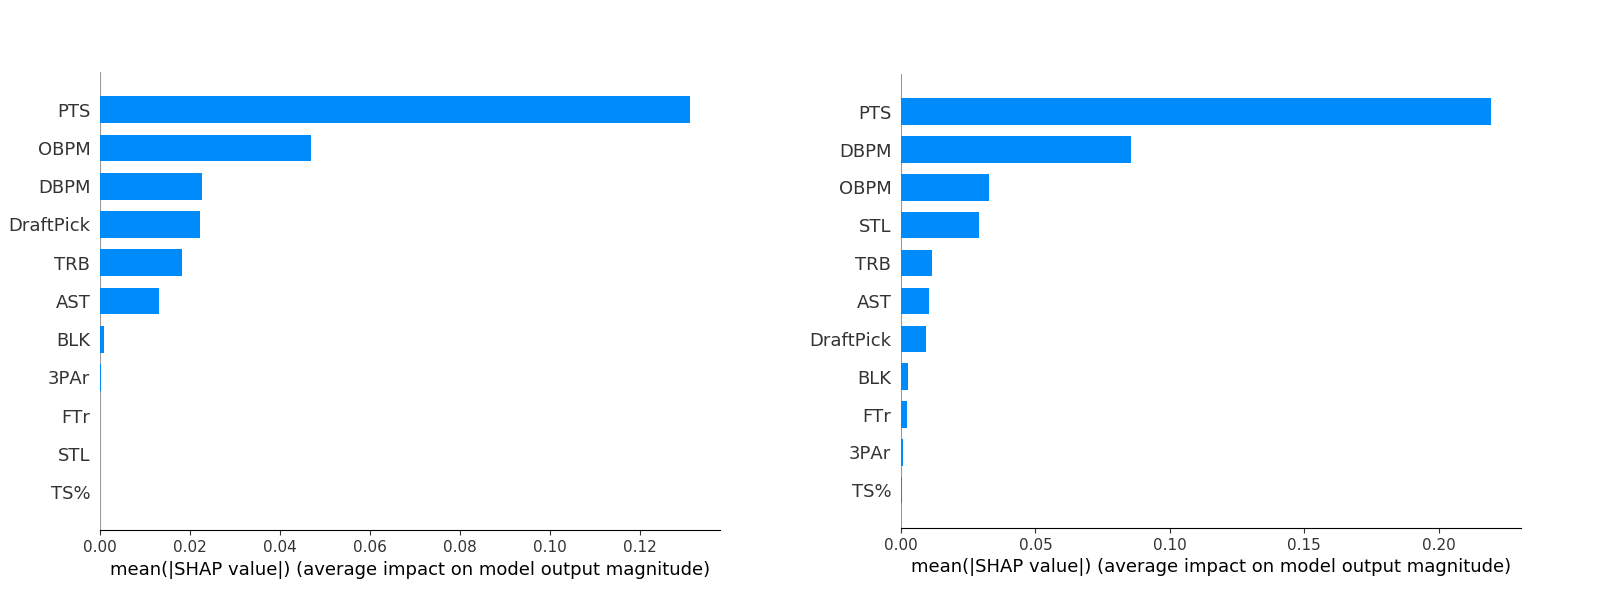
\includegraphics[scale=0.3]{svm_shap.png}
\end{center}
\caption{SHAP values for SVC for accuracy (left) and recall (right)}
\label{plt:shap_svm_all_star}
\end{figure}

\begin{figure}[h!]
\begin{center}
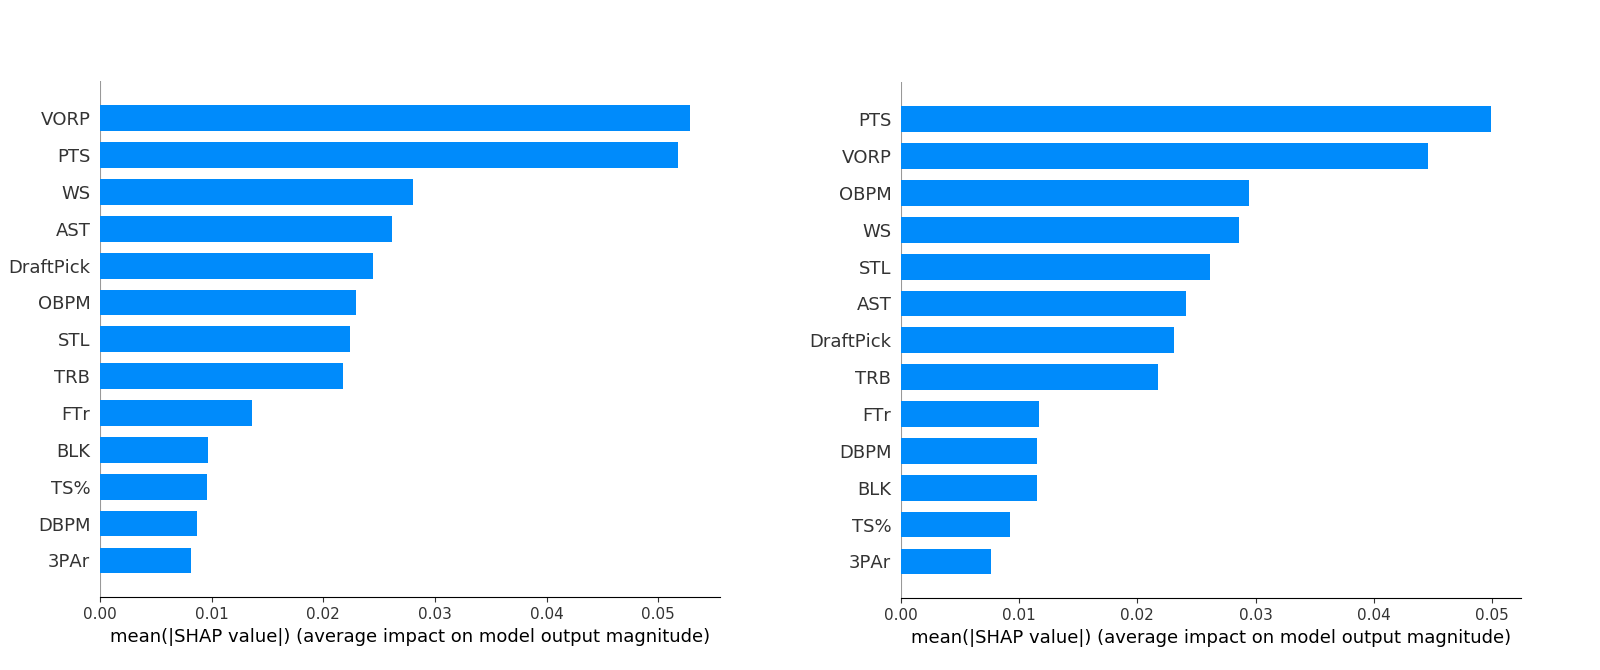
\includegraphics[scale=0.3]{rfc_shap.png}
\end{center}
\caption{SHAP values for RFC for accuracy (left) and recall (right)}
\label{plt:shap_rfc_all_star}
\end{figure}

\begin{figure}[h!]
\begin{center}
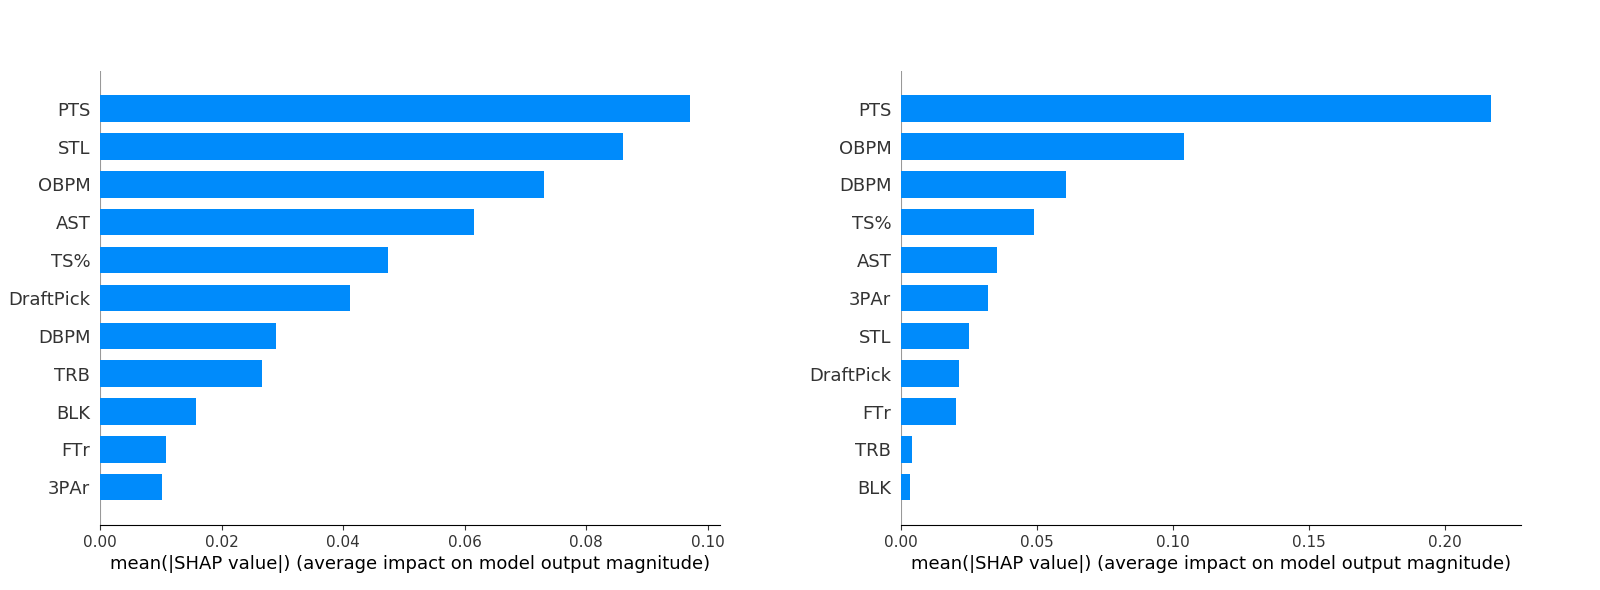
\includegraphics[scale=0.3]{gbc_shap.png}
\end{center}
\caption{SHAP values for GBC for accuracy (left) and recall (right)}
\label{plt:shap_gbc_all_star}
\end{figure}

\subsubsection{Models without draft pick taken into consideration}
\label{subsubsec:without_draft_pick_all_star}

After finishing classification and showing the results, one question remains. Why should player's position on the draft have influence on his chance of becoming an All-Star. I mean, players that are believed to be better prospects will be selected higher, so a player drafted number one overall should have higher probability of being an All-Star than the player selected 14th. But, after they enter the league the way they are playing matters, not their draft position. Because of that, more models will be created, using the same stats but this time \textbf{draft position will be excluded}!

Process of creating and testing the models is the same as before, six models in total, three with the best accuracy (SVC, RFC and GBC) and three with the best recall, also SVC, RFC and GBC. Model parameters are again selected with grid search.

Models will be trained on the same data as before (stats from the 2000 NBA draft to 2016 NBA draft) and will applied to the same data as models created earlier (20017 and 2018 NBA drafts). Models can be seen in table \ref{tab:models_no_draft_pick_all_star}.

\begin{table}[!h]
\begin{center}
\begin{tabular}{|c|c|c|c|c|} \hline
\multicolumn{5}{|c|}{\textbf{Models with the best accuracy}} \\ \hline
\textbf{Model} & \textbf{Accuracy} & \textbf{Precision} & \textbf{Recall} & \textbf{F1 score} \\ \hline
SVC & \textbf{0.81} & 0.72 & 0.67 & 0.69 \\ \hline
RFC & \textbf{0.85} & 0.80 & 0.72 & 0.75 \\ \hline
GBC & \textbf{0.82} & 0.74 & 0.68 & 0.70 \\ \hline
\multicolumn{5}{|c|}{\textbf{Models with the best recall}} \\ \hline
\textbf{Model} & \textbf{Accuracy} & \textbf{Precision} & \textbf{Recall} & \textbf{F1 score} \\ \hline
SVC & 0.81 & 0.72 & \textbf{0.67} & 0.69 \\ \hline
RFC & 0.85 & 0.80 & \textbf{0.72} & 0.75 \\ \hline
GBC & 0.82 & 0.74 & \textbf{0.68} & 0.70 \\ \hline
\end{tabular}
\caption{Models created without draft pick}
\label{tab:models_no_draft_pick_all_star}
\end{center}
\end{table}

Note that SVM with the best accuracy and SVM with the best recall are the models with the same parameters, according to grid search. Same applies to RFC, but not to GBC. These models have similar results as the ones with draft pick taken into consideration, so maybe the probabilities won't be different much. Other test won't be shown and instead of them we will go to the results right away (table \ref{tab:results_no_draft_pick_all_star}).

\begin{table}[!h] % the best accuracy models average
\begin{center}
\begin{tabular}{|c|c|c|c|c|} \hline
\textbf{ } & \textbf{ } & \textbf{Accuracy} & \textbf{Recall} & \textbf{Average} \\
\textbf{Pick} & \textbf{Player} & \textbf{models} & \textbf{models} & \textbf{of every} \\
\textbf{ } & \textbf{ } & \textbf{average} & \textbf{average} & \textbf{model} \\ \hline
1 & Markelle Fultz & 0.12 & 0.11 & 0.12 \\ \hline
2 & Lonzo Ball & 0.50 & 0.50 & 0.50 \\ \hline
3 & Jayson Tatum & 0.67 & 0.67 & 0.67 \\ \hline
4 & Josh Jackson & 0.18 & 0.18 & 0.18 \\ \hline
5 & De'Aaron Fox & 0.16 & 0.15 & 0.15 \\ \hline
6 & Jonathan Isaac & 0.11 & 0.10 & 0.10 \\ \hline
7 & Lauri Markkanen & 0.25 & 0.25 & 0.25 \\ \hline
8 & Frank Ntilikina & 0.14 & 0.13 & 0.14 \\ \hline
9 & Dennis Smith & 0.40 & 0.40 & 0.40 \\ \hline
10 & Zach Collins & 0.10 & 0.10 & 0.10 \\ \hline
11 & Malik Monk & 0.04 & 0.03 & 0.04 \\ \hline
12 & Luke Kennard & 0.08 & 0.07 & 0.07 \\ \hline
13 & Donovan Mitchell & 0.68 & 0.68 & 0.68 \\ \hline
14 & Bam Adebayo & 0.15 & 0.15 & 0.15 \\ \hline
1 & Deandre Ayton & 0.78 & 0.78 & 0.78 \\ \hline
2 & Marvin Bagley & 0.21 & 0.21 & 0.21 \\ \hline
3 & Luka Dončić & 0.91 & 0.91 & 0.91 \\ \hline
4 & Jaren Jackson & 0.55 & 0.55 & 0.55 \\ \hline
5 & Trae Young & 0.54 & 0.54 & 0.54 \\ \hline
6 & Mo Bamba & 0.09 & 0.08 & 0.09 \\ \hline
7 & Wendell Carter & 0.17 & 0.17 & 0.17 \\ \hline
8 & Collin Sexton & 0.14 & 0.13 & 0.14 \\ \hline
9 & Kevin Knox & 0.16 & 0.16 & 0.16 \\ \hline
10 & Mikal Bridges & 0.17 & 0.17 & 0.17 \\ \hline
11 & Shai Gilgeous-Alexander & 0.20 & 0.20 & 0.20 \\ \hline
12 & Miles Bridges & 0.08 & 0.08 & 0.08 \\ \hline
13 & Jerome Robinson & 0.03 & 0.03 & 0.03 \\ \hline
\end{tabular}
\caption{Results without draft pick taken into consideration}
\label{tab:results_no_draft_pick_all_star}
\end{center}
\end{table}


Results are indeed somewhat similar. Luka Dončić remained the player most probable to become an All-Star. As the ones before, these models value Tatum, Mitchell and Ayton. We can also see that the probability of Bagley becoming an All-Star decreased, while probability of Jeren Jackson becoming an All-Star increased. Lonzo Ball and Dennis Smith  also got their chances increased. There are not significant changes for the players that are selected late in the lottery. Note that, once again, Ayton's season is valued the highest out of all other seasons of the players that have yet to officially become an NBA All-Star.

This models confirms that Sacramento Kings should have selected Dončić instead of Bagley number two overall on 2019 NBA draft. Models are not valuing New York's young core of Smith, Ntilikina and Knox. Orlando's rookies are also not looking good judging by this model. As we have already said, things can change, and rookies can and will improve, so don't take these results as an absolute measurement.

\pagebreak

\addcontentsline{toc}{section}{References}
\appendix
\bibliography{ref}
\bibliographystyle{unsrt}
\appendix

\end{document}
